\documentclass[12pt]{article}
\usepackage{graphicx,subfigure}
\usepackage{hyperref,amsmath,fancyhdr}
\usepackage[usenames,dvipsnames]{color}
\usepackage{supertabular, listings}
\usepackage[english]{babel} 
%\usepackage[left=2.0cm, right=2.0cm, top=2.5cm, bottom=2.5cm, headsep=1.2cm]{geometry}
\usepackage{amscd,amssymb,verbatim}
%\usepackage[TS1,OT1,T1]{fontenc}
\usepackage{cite}
\usepackage{eurosym}
\usepackage{array}
\usepackage{hyperref}
\usepackage{fancyvrb}
\usepackage{multirow}
\usepackage[titletoc]{appendix}
%\usepackage{ccaption}
\pagestyle{headings}
\usepackage{subfigure} 
\usepackage{color}
\usepackage{spverbatim}
\usepackage{lscape}
\usepackage{hhline}

 
\textheight 23cm
\textwidth 17.5cm
\topmargin -1.0cm
\hoffset -2.0cm

%\newfixedcaption{\figcaption}{figure}

\begin{document}

\begin{titlepage}
\centering
{{\Huge\bf \sffamily MINT}}\\
\vspace{0.35cm}
{{\Huge\bf \sffamily version 1.0.1}}\\
\vspace{0.5cm}
{{\Huge\bf \sffamily Users' Manual}}\\
\vspace{1cm}
{\large{\bf{\sffamily Anna G\'{o}rska}}}\\
{\large{\bf{\sffamily Maciej Jasi\'{n}ski}}}\\
{\large{\bf{\sffamily Joanna Trylska}}}\\
\vspace{2cm}

\includegraphics[width=0.4\textwidth]{./pictures/Mint.png}\\
\vspace{0.2cm}

\includegraphics[width=0.3\textwidth]{./pictures/logoLMB.png}
\end{titlepage}
\newpage
     {\sffamily{MINT is a free software; you can redistribute it and/or modify 
     it under the terms of the GNU General Public License version 2,  
     as published by the Free Software Foundation.\\
     \\                                                                       
     This program is distributed in the hope that it will be useful,        
     but WITHOUT ANY WARRANTY; without even the implied warranty of       
     MERCHANTABILITY or FITNESS FOR A PARTICULAR PURPOSE.  See the GNU General Public License for more details.\\                          
     \\                                                                       
     You should have received a copy of the GNU General Public License    
     along with this program; if not, write to the                         
     Free Software Foundation, Inc.,                                      
     59 Temple Place - Suite 330, Boston, MA  02111-1307, USA.\\
     \\
     \vspace*{1cm}
     Copyright (C) 2013 -- 2014: University of Warsaw}}  
\includegraphics[width=0.1\textwidth]{./pictures/logoUW.png}

\newpage
\tableofcontents
\newpage
\newcommand*{\elem}[1]{{\color{Gray}{\tt{<#1>}}}}
\newcommand*{\greyT}[1]{{\color{Gray}{\tt{#1}}}}

\section{Introduction}
{\tt MINT} (Motif Identifier for Nucleic acids Trajectory) is an automatic tool for reading and analyzing three-dimensional structures of nucleic acids, their molecular dynamics trajectories (written in CHARMM, Gromacs, NAMD, LAMMPS, or different formats) or other conformation sets.\\

\noindent
{\tt MINT} deals with both DNA and RNA molecules. However, since mainly RNAs acquire complicated 3D folds, we write this manual in the context of RNA. The analysis includes hydrogen bonding, stacking and secondary-structural motifs. For many conformations of the same nucleic acid molecule {\tt MINT} provides various physicochemical properties as a function of simulation time (or frame), as well as statistics providing an overall-view of the changes in these properties occuring in the inputted conformation set (e.g., trajectory).\\

\noindent
Please direct your comments and questions about the {\tt MINT} package to:\\
{\tt{agorska@cent.uw.edu.pl}} or {\tt{m.jasinski@cent.uw.edu.pl}}\\
Centre of New Technologies,
University of Warsaw\\
Banacha 2c, 02-097 Warsaw, Poland\\
phone:  $+$48 22 5543 683 \\ 
\\
The web interface to analyze the PDB files containing single RNA or DNA structure and the source code of the {\tt MINT} package to analyze multiple conformation sets (for example, molecular dynamics trajectories) is available at:\\
\\
{\color{Blue}{\tt{http://mint.cent.uw.edu.pl}}}\\
\\
\noindent
or can be accessed via:\\
\\ 
{\color{Blue}{\tt{https://bionano.cent.uw.edu.pl/Software}}}\\
\\
{\tt MINT} is distributed under the terms of the GNU Public License. 
A copy of the GPL is provided with the distribution and is also available at {\color{Blue}\tt{http://www.gnu.org}}. \\

\subsection{Citing MINT}
\noindent
If you find this software useful please cite: Anna G\'{o}rska, Maciej Jasi\'{n}ski, Joanna Trylska, 
\textit{MINT: software to identify motifs and short-range interactions in trajectories of nucleic acids}. Nucleic Acids Res. 2015 May 29. doi: 10.1093/nar/gkv559 PubMed PMID: 26024667. 
\newpage
\section{Quick reference}
\subsection{What can {\tt MINT} do?}

\textbf{For a single PDB file of an RNA/DNA molecule {\tt MINT} provides:}
\begin{itemize}
\item regions forming helices,
\item regions forming loops, bulges, interior loops, junctions,
\item regions forming pseudoknots,
\item nucleotides creating triplets,
\item all Watson-Crick edge base pairs,
\item all non-Watson-Crick edge base pairs,
\item all stacking and anion-$\pi$ interacting nucleotides,
\item the number of Watson-Crick edge hydrogen bonds per nucleotide,
\item the number of non-Watson Crick edge hydrogen bonds per nucleotide,
\item the stacking energy -- Van der Waals and electrostatic energies and their sum per nucleotide,
\item visualizations of the computed parameters.
\end{itemize}

\noindent
\textbf{For trajectory (or set of conformations) of the RNA/DNA molecule (e.g., derived from molecular dynamics trajectory) {\tt MINT} provides:}
\begin{itemize}
\item residues forming helices, triplets, pseudoknots and other motifs, 
\item all base-pairs: Watson-Crick edge and non-Watson-Crick edge, along with the conformation,
\item clusters of secondary structure motifs and average motifs along with hydrogen bonding (in Watson-Crick edge and non-Watson-Crick edge contacts),
\item all stacking, anion-$\pi$ interacting nucleotides, 
\end{itemize}
All of the detected structures/motifs is described also with its occurrence in the trajectory: percentage of frames and their specyfic numbers. How often given structure was present in the trajectory is a measurement of its stability.

{\tt MINT} computes also various global parameters for a given trajectory:
\begin{itemize}
\item the average number of Watson-Crick and non-Watson Crick edge hydrogen bonds per nucleotide,
\item the average stacking energy -- Van der Waals and electrostatic energies, their sum per nucleotide,
\item average secondary structure,
\item visualizations of the above listed parameters (see section \ref{Visualization})
\end{itemize}

\subsection{What do you need to run {\tt MINT}?}
\begin{itemize}
\item {\tt Python2.7} and external python packages: {\tt  numpy, BioPython, MDAnalysis, xlwt} and {\tt  pympler}. For details see section~\ref{external_pack}.
\item a PDB file with a full-atom RNA structure (including hydrogens).
\item a trajectory file (e.g. in the .dcd format) to use the {\tt Traj} mode.
\item a version 1.6+ of the {\tt JAVA Virtual Machine} to run {\tt VARNA}~\ref{varna} the visualiztion applet that {\tt MINT} uses to generate secondary structure pictures.
\end{itemize}

\subsection{Definitions}
Here we outline a few concepts/definitions used in this manual and software. 
\begin{itemize} 
\item Secondary contacts -- both nucleotides interact with the Watson-Crick edge (WC), see Figure \ref{Edges}.
\item Tertiary contacts -- at least one of the nucleotides interacts with its non-Watson-Crick edge (non-WC), see Figure \ref{Edges}.
\item RNA secondary structure -- a structure created by the WC base pairs, excluding pseudoknots, as in the standard dot-bracket notation.
\item RNA tertiary structure -- a structure created only by non-WC pairs.
\item Motif -- a loop, a bulge or junction; a helix is treated as a separate entity.
\end{itemize}

\section{Installation} \label{external}
\subsection{Required external python packages} \label{external_pack}
Despite the {\tt python 2.7} (\url{http://python.org}), {\tt MINT} uses also some external packages:

\begin{itemize}
\item  {\tt numpy} --  the package with tools to manipulate multi-dimensional arrays (\url{http://www.scipy.org/Download}).
\item  {\tt BioPython} -- the main package for loading and managing the PDB structures (\url{http://biopython.org/wiki/Main_Page}).
\item  {\tt MDAnalysis} \cite{Denning2012} -- used for reading the trajectory (\url{http://code.google.com/p/mdanalysis/wiki/Install}).
\item  {\tt xlwt} -- the package for writing .xls files. It is used by {\tt csvToxls.py} script to write all output .csv files into the .xls files (\url{https://pypi.python.org/pypi/xlwt}).
\item  {\tt pympler} -- the package determining the memory usage of the objects in the python script (\url{http://pythonhosted.org/Pympler}). 
\item if you wish to use {\tt CORRELATIONS.py} script (see paragraph \ref{CorrelationsParagraph}), you should install {\tt matplotlib} python package: \url{http://matplotlib.org}. 
\end{itemize}

All of the required packages have their home websites (provided in brackets above) where they can be downloaded from along with instructions. All of them can also be installed through {\tt easy\_install}, that is provided by the {\tt setup\_tools} package (\url{https://pythonhosted.org/setuptools/easy_install.html#installing-easy-install}):

\begin{verbatim}
 easy_install numpy  
 easy_install Biopython
 easy_install MDAnalysis
 easy_install xlwt
 easy_install pympler
\end{verbatim}

%\paragraph{multipy}
If you encounter problems with installing {\tt python2.7} or required packages, you can use the {\tt Multipy} package. {\tt Multipy} enables to set up a local virtual python environment and run any {\tt python} script. You can download multipy from: (\url{http://code.google.com/p/multipy/} or \url{https://github.com/akheron/multipy}). \\

First, to install {\tt python 2.7} in the multipy enviroment, type:
\begin{verbatim}
multipy install 2.7
\end{verbatim}
then you can access the {\tt python 2.7} multipy environment  by using:
\begin{verbatim}
 bash
 . $(multipy activate 2.7)
\end{verbatim}
and second, install the required packages inside the environment, using  {\tt easy\_install} as in the example above.

\subsection{MINT}
Download and unpack the {\tt MINT.tar.gz} package from the webpage:
\newline{\color{Blue}{\tt{http://mint.cent.uw.edu.pl/index.php?strona=MintDownload}}}\\


\section{Running {\tt MINT}}
Go to the {\tt MINT} directory and type:
\begin{verbatim}
python MINT.py CONFIG_traj.MINT
\end{verbatim}
and the program will perform a short run for the {\tt example.pdb} and {\tt example.dcd}, present in the {\tt MINT/example} folder (see Section \ref{Example_sec}), with all parameters set to their default values. Results will be placed in the {\tt MINT/example-traj} folder. If any error appears check whether you are using {\tt python 2.7} and have all the required packages installed (see Section \ref{external_pack}).

{\tt MINT} uses a simple text configuration file, which specifies input parameters. Each line in the configuration file consists of a keyword identifying the parameter and its value. Comments are denoted by the {\tt \#} character. The syntax is:
\begin{verbatim}
keyword:option # comment
\end{verbatim}


\subsection{Analysing the DNA versus RNA structures}
{\tt MINT} includes necessary parameters for analysing both DNA and RNA molecules. By default {\tt MINT} distinguishes the DNA molecules by the names of the residues in the input PDB file, it expects the DNA nucleotides to be named: Adenine: DA, Guanine: DG, Cytosine: DC, Thymine: DT. Other nucleotides will be treated as RNA or derivatives. 
However, with the option {\tt all\_nucs\_DNA: 1} it's possible to force MINT to treat all standard nucleotides as DNA. 

\subsection{Parameters specified in the {\tt CONFIG.MINT} configuration file}
\begin{itemize}
\item {\tt Mode} -- [Single/Traj/Download] determines whether a trajectory or  single structure %or list of PDB deposited structures 
will be analyzed. In the Single mode, only the conformation from the PDB file {\tt file\_name} parameter will be analyzed. In the Traj mode conformations from the {\tt file\_dcd} file will be analyzed. 
%In the Download mode {\tt MINT} will download, protonate and analyze all PDB deposited structures specified in {\tt pdb\_list} parameter. 
\item {\tt out\_name} -- [directory and/or file name] specified file name will be the prefix for all of the output files. You can also add a relative path to the directory in which you want outputs to be created (e.g. specifying {\tt ./foo/bar} you will place your output files with {\tt bar\_} prefix in the {\tt ./foo} directory).
\item {\tt file\_name} -- [file name] input PDB file containing nucleic acid structure. The file is required in both Single or Traj modes.
\item {\tt file\_dcd} -- [file name] input file containing multiple conformations, trajectory for the Traj mode. The supported trajectory formats {\tt are .dcd .xyz .trr .crd} as in the {\tt MDAnalysis} package.  
\item {\tt chains\_names} -- [list] the list of chain ids to be analyzed. If it is empty, the analysis will be performed for all chains. \textbf{Note, that for analysis all provided chains are treated as a single chain.}
\item {\tt first\_frame} -- [int] the number of the first frame to be analyzed from the trajectory file. {\bf Note, that numbering starts from 0}.
\item {\tt last\_frame} -- [int/-1] the number of the last frame to be analyzed in the trajectory, if set to -1 the program replaces it with the number of the last frame.
\item {\tt stride} -- [int] the number specifies how many frames to skip between two analyzed frames. When set to 0 the whole trajectory will be analyzed. 
\item {\tt cutoff} -- [\AA] the cutoff for the distance measured between the C1' carbons of every nucleotide. For nucleotides located in distance larger than {\tt cutoff} the program does not search for hydrogen bonds. Default is {\tt 20}.
\item {\tt cutoff\_stacking} -- [\AA] the cutoff for the distance  measured between the the centers of mass of every nucleobase. For nucleotides placed in distance larger than {\tt cutoff\_stacking} the program does not search for the stacking interaction. Default is {\tt 10.5}.
\item {\tt vdw\_cutoff\_stacking} --  [kcal/mol] the maximal value of the Van der Waals (VDW) energy for the stacking interaction. If the VDW energy between two nucleobases is smaller than the given {\tt vdw\_cutoff\_stacking} parameter, the stacking interaction is detected. Default value: {\tt -0.5}.
\item {\tt OP\_stacking\_distance\_cutoff} -- [\AA]  the maximal distance between a backbone phosphate group and a nucleobase center of mass for the calculation of the anion-$\pi$ interaction. If measured distance is smaller than given {\tt OP\_stacking\_distance\_cutoff} parameter the anion-$\pi$ interaction is detected. Default is {\tt 4.5}.
\item {\tt h\_bond\_atom} -- [donor/hydrogen] indicates whether the hydrogen bond distance should be computed between a {\bf donor} and acceptor or a {\bf hydrogen} and acceptor.
\item {\tt h\_bond\_l} -- [\AA] the maximal length  of the hydrogen bond. Default value of {\tt 4} was set with {\tt h\_bond\_atom:donor}.
\item {\tt h\_bond\_angle}  -- [degrees] the minimal angle of the hydrogen bond. Default is {\tt 140}.
\item {\tt vmd} -- [0/1] the binary parameter working only in {\tt SingleOrTraj:Single} mode. If set to 1 a~{\tt VMD} application will be opened and the input structure coloured by secondary structures. This is possible only if {\tt VMD} is properly installed and added to PATH (alternatively, it can be run from command line, see Section \ref{VMD}).
\item {\tt table\_nucleotides} -- [file name] the {\tt .csv} file determining the hydrogen donors, acceptors and nucleotide edges for every nucleotide. By editing this file, one can remove certain interactions from the analysis or define new types of interactions. Default file {\tt nucleotides\_modified.csv} is stored in the {\tt MINT/data} folder.
\item {\tt table\_charges}  -- [file name] the {\tt .csv} file listing the partial charges, Van der Waals radii and depths of the Lennard-Jones potential for atoms in nucleotides. These parameters are given for two force fields: AMBER~\cite{Wang2000} and CHARMM~\cite{Mackerell2000,Foloppe2000}, but there is also a column MY\_OWN for the user to put other parameters if needed. 
Default file {\tt ./data/charges\_and\_VDW\_modified.csv} is stored in the {\tt MINT/data/} folder.
\item {\tt list\_of\_modified\_nucs} -- the two-column text file with the list of modified RNA nucleotides present in the RNA structures deposited in the PDB database (as of July 2014). Each row contains the residue name used for the modified nucleotide and a single-letter code (a, g, c, t, u) for the natural nucleotide from which the modification originates. Default {\tt data/unknown\_modified.fa} is stored in the {\tt MINT/data} folder.
\item {\tt force\_field} --  [AMBER/CHARMM/MY\_OWN] the name of the force field to be used by the program while computing stacking energies.
\item {\tt margin} -- [0.0 -- 1.0]  the minimal portion of nucleotides that have to be common for both motifs to belong to the same cluster. Default is {\tt 0.8}.
\item {\tt time\_cutoff} -- [0.0 -- 1.0] the minimal portion of the conformations (part of the frames) from the trajectory where the motifs must be present in order to be incorporated into the cluster analysis. Default is {\tt 0.02}.
\item {\tt max\_memory\_GB} -- [GB] the maximal memory the single thread is allowed to use at one time. Default is {\tt 1.5}.
\item {\tt threads} -- [int] the number of CPUs to be used while analyzing  the trajectory. Default is~{\tt 1}.
\item {\tt only\_analysis} -- [1/0] if 1, the program instead of running the whole analysis, reads the previously performed analyses, performs computations only for the missing frames and creates output files. You can turn on this parameter if your computations were disturbed for some reason. In this mode {\tt MINT} uses only one CPU. Default is {\tt 0}.
%\item {\tt pdb\_list} -- [string] list of the PDB codes in line separated by space. For each {\tt MINT} will download the structure from the PDB database, unpack, protonate using the {\tt reduce} program~\cite{Word1999a} and perform the analysis in a single frame mode. Every analysis will be automatically located in a separate directory. 
\item {\tt create\_csvs}  -- [1/0] if 1, MINT will create separate csv file for each sheet present in the {\tt \_MINT.xls} output file. Only nonempty sheets and files are made. When analyzing very long trajectories {\tt MINT} may produce csv files, even if the parameter is set to 0. This is related to the limitation of the .xls file format. In such case there will be a reference in the .xls file to see the .csv files.
\item {\tt pairing\_cutoff} -- [0.0 -- 1.0] the minimal portion of the conformations (part of the frames) from the trajectory where pair must be present in order to be incorporated into the {\tt pairing} table. Default is~{\tt 0.1}.
\item {\tt all\_nucs\_DNA} -- [1/0] if 1, MINT will treat all standard nuceotides as DNA instead od RNA. Default is~{\tt 0}.
\item {\tt write\_nucs\_timeseries} -- [1/0] if 1, MINT will save hydrogen bonds and stacking interaction analysis vs time in csv files. Requires installation of additional {\tt python} library: {\tt pandas}. Default is~{\tt 0}.
\end{itemize}


\subsection{Example} \label{Example_sec}
The {\tt example} directory of {\tt MINT} contains the following inputs:
\begin{itemize}
\item {\tt example.pdb}  -- a .pdb file with the atomic structure of the RNA molecule. One will benefit from the program mostly by analyzing RNA structures with complex secondary and tertiary structures.
\item {\tt example.dcd}  -- a trajectory file containing ten frames from molecular dynamics simulations performed with NAMD \cite{Phillips2005} and using the CHARMM force field.
\end{itemize}

In the  {\tt example-traj} following \textbf{outputs} are present:
\begin{itemize}
\item Structure description (see section \ref{OutputFiles} for details):
\begin{itemize}
\item  example\_MINT\_description.txt	
\item example\_MINT.xls
\item example\_nucleotides\_characteristics.csv
\item example\_pairs.csv
\item example\_pairing.csv
\item example\_helices.csv
\item example\_motifs.csv
\item example\_average\_motifs.csv				
\item example\_motifs\_clusters.csv
\item example\_stacking.csv
\item example\_pi\_interactions.csv
\item example\_dot\_bracket.txt
\end{itemize}
\item Visualization, secondary structure movie  (see section \ref{Visualization} for details):
\begin{itemize}
\item example\_RNAStructML.xml
\end{itemize}
\item Visualization, PDB:
\begin{itemize}
\item example\_Hbonds-WC.pdb				
\item example\_Hbonds-non-WC.pdb				 
\item example\_Hbonds-total.pdb				 
\item example\_Stacking-VDW.pdb				
\item example\_Stacking-Coulomb.pdb
\item example\_Stacking-total.pdb
%\item vmd\_run.tcl
\end{itemize}
\item Visualization, pictures:
\begin{itemize}
\item example\_Hbonds-WC.png				
\item example\_Hbonds-non-WC.png
\item example\_Hbonds-total.png		 
\item example\_Stacking-VDW.png				
\item example\_Stacking-Coulomb.png
\item example\_Stacking-total.png
\end{itemize}
\end{itemize}

All the examples provided in this manual are derived from above files.

\section{Output files}\label{OutputFiles}
{\tt MINT} generates multiple files both in the single frame analysis mode and in the trajectory mode. Names of the generated files begin with the {\tt out\_name} parameter value. 
The output files describe nucleotides in the way that they can be unambiguously identified. We use the representation containing a chain name, a residue name and its number. For example: the {\tt N|GUA:521} represents the residue number 521 from the chain N, with the name GUA. The values posted in the {\tt chain name|residue name:residue number} code are derived from the input PDB file.

\subsection{description.txt}
The {\tt \_description.txt} file contains a complete description of the structure for every analyzed frame. The exemplary description is shown in the end of this manual. The single frame description contains a complete list of used parameters, helices, motifs, triplets, pseudoknots. One can also find a list of  WC, non-WC pairs, stacking and $\pi$ interactions and their exact parameters, as well as a~dot-bracket representation of the secondary structure. The frames are separated by the headers: {\tt frame number}.

\subsection{MINT.xls}
The {\tt \_MINT.xls} file is a complete .xls (spreadsheet type) file collecting all calculated properties in separated sheets. If the {\tt create\_csvs} parameter is set to 1 a {\tt .csv} file will be created for every present sheet. Only non-empty files/sheets are produced. 
In the first sheet of the {\tt \_MINT.xls}  there is a legend explaining used sheet names.
In the {\tt Trajectory} mode of analysis the following columns are present in selected output sheets/files:
\begin{itemize}
\item {\tt  \% of frames} -- contain percentage of frames when a motif/pair/interaction was present, describes in how many frames of the trajectory given structure (e.g. a pair) was present. It is a measure of the stability of the interaction.
\item {\tt frame numbers} --  contain frame numbers in which a motif/pair/interaction was present. The notation $ 2\rightarrow 15$ $20\rightarrow 26$ denotes that the structure can be found in frames number 2,3,4.. up to 15, and than frames number 20 to 26.
\end{itemize}

Below there is a description of the sheets forming the {\tt \_MINT.xls} file:
\subsubsection{Pairs}  
The {\tt pairs} sheet is a table containing all nucleobase pairs that appeared during the trajectory. The sheet contains the following columns: {\tt 1st nucleotide number}, {\tt nucleotides}, {\tt pair type} classified according to the interacting edges (e.g. WC-WC), {\tt pair configuration} (\textit{cis} or \textit{trans}), {\tt vmd}, {\tt \% of frames}, {\tt frame numbers}, the exemplary data record is shown below:
\begin{table}[h!]
\begin{tabular}
{ | >{\centering} m{2cm} | >{\centering} m{2.2cm} | >{\centering} m{2.8cm}  | >{\centering} m{2.2cm} | >{\centering} m{2.5cm} |>{\centering} m{1.5cm} |>{\centering} m{2cm} |}  \hline 
1st nucleotide number & nucleotides	& pair type	&  pair configuration & vmd & \% of frames & frames numbers \tabularnewline \hline \hline
515&	N$|$G:515/ N$|$C:536 &WC/WC& Cis& chain N and resid 515 536	& 100\%	& $0\rightarrow 9$  \tabularnewline \hline
516&	N$|$U:516/ N$|$C:519&WC/Hoogsteen& Trans & chain N and resid 516 533& 50\% &	  $3$, $6\rightarrow 8$   \tabularnewline \hline
522&	N$|$C:522/ N$|$G:527&WC/WC&Cis& chain N and  resid 522 527 &	100\% & $0\rightarrow 9 $ \tabularnewline \hline
\end{tabular}
\caption{Example of the {\tt pairs} table.}
\end{table}
%\newpage

\subsubsection{Pairing} 
The {\tt pairing} sheet is a table enlisting the hydrogen bonding partners for every nucleotide. The {\tt pairing\_cutoff} parameter specifies the minimal part of frames in which pair has to be present in order to be taken into account.
The partners are enlisted vertically and than coded: number of hydrogen bonds - nucleotide (chain$|$name:number) - number of frames. See the example below:
\begin{table}[h!]
\begin{tabular}
{| >{\centering} m{2.5cm} | >{\centering} m{2cm} | >{\centering} m{3.5cm}  | >{\centering} m{3.5cm} | }  \hline
nucleotide number&nucleotide&interaction&interaction \tabularnewline \hline \hline
500&N$|$G:500&3-N$|$C:545-5&\tabularnewline \hline
501&N$|$C:501&2-N$|$G:544-3&3-N$|$G:544-2\tabularnewline \hline
502&N$|$A:502&2-N$|$U:543-1&3-N$|$U:543-4\tabularnewline \hline
\end{tabular}
\caption{Example of the {\tt pairing} table.}
\end{table}
The C nucleotide number 501 from chain N was forming 2 hydrogen bonds with G number 544 in 3 frames and 3 hydrogen bonds with the same partner in 2 frames. 

\subsubsection{Secondary structure motifs} 
There are separate sheets created for different types of the secondary structure motifs:
\begin{itemize}
\item {\tt helices},
\item {\tt pseudoknots},
\item {\tt triplets},
\item {\tt motifs}. 
\end{itemize}
Each of them contains the following columns: 
\begin{itemize}
\item {\tt nucleotides}  - nucleotides forming the motif,
\item {\tt vmd} - ready to paste into the {\tt VMD} residual identifiers,
\item {\tt \% of frames}, 
\item {\tt frame numbers}.
\end{itemize} 
The  {\tt motifs} sheet contains also a {\tt motif\_topology} collumn -- for explanation see \ref{RNA_motifs}.
Below there is an example of the motifs table:
\begin{table}[h!]
\begin{tabular}
{ | >{\centering} m{1.5cm} | >{\centering} m{5cm} | >{\centering} m{6.5cm}  | >{\centering} m{1.5cm} | >{\centering} m{2cm} |}  \hline
motif topology	& nucleotides &VMD& \% of frames & frame numbers  \tabularnewline \hline \hline
7-5	 & N$|$G:515-N$|$C:536 ... N$|$U:516-N$|$G:515	 & chain N and resid 515 536 .. 516 515 & 100\% & $0 \rightarrow 9 $ \tabularnewline \hline
4 & N$|$C:522-N$|$G:527 ... N$|$A:523-N$|$C:522& chain N and resid 522 527 .. 523 522 & 100\%	& $ 0\rightarrow  9 $ \tabularnewline \hline
0-6 & N$|$C:504-N$|$G:541 ... N$|$G:505-N$|$C:504	& chain N and resid 504 541 .. 505 504 & 100\% & $ 0\rightarrow 9$ \tabularnewline \hline
\end{tabular}
\caption{Example of the {\tt motifs} table.}
\end{table}

\subsubsection{{Stacking}}
The {\tt stacking} sheet is table containing all the nucleotide pairs recognized as stacked. The table contains the following columns: {\tt 1st nucleotide number}, {\tt nucleotides}, {\tt Coulomb avg}, {\tt Coulomb sd} (the Coulomb interaction energy in kcal/mol followed by its standard deviation),	{\tt VDW avg}, {\tt VDW sd} (the VDW interaction energy in kcal/mol followed by its standard deviation), {\tt Stacking-total avg}, {\tt Stacking-total sd} (sum of the VDW and Coulomb interactions for the recognized pair in kcal/mol with the standard deviation value), {\tt vmd}, {\tt \% of frames} and {\tt frame numbers}. In case of analyze of the single structure, columns with the standard deviations values will not be present. Example of the {\tt stacking} sheet is presented below. 

\begin{table}[h]
\footnotesize
\begin{tabular}
{| >{\centering} m{1.2cm} | >{\centering} m{1.5cm} | >{\centering} m{1.3cm} | >{\centering} m{1.3cm} | >{\centering} m{1.1cm} | >{\centering} m{1.1cm} | >{\centering} m{1.4cm} | >{\centering} m{1.4cm} | >{\centering} m{1.3cm} | >{\centering} m{1.3cm} |  m{1.3cm} |}
\hline
1st nucleotide number & nucleotides         & Coulomb avg & Coulomb sd & VDW avg & VDW sd & Stacking-total avg & Stacking-total sd & VMD                        & \% of frames & frame numbers   \tabularnewline \hline  \hline
509                   & N$|$A:509/ N$|$A:510 & 25.64       & 2.25       & -5.52   & 0.61   & 20.11              & 2.33              & chain N and resid  509 510 & 100.00\%     & 0-\textgreater9 \\ \hline
501                   & N$|$C:501/ N$|$A:502 & 6.23        & 1.80       & -2.65   & 0.55   & 3.58               & 1.88              & chain N and resid  501 502 & 100.00\%     & 0-\textgreater9 \\ \hline
503                   & N$|$C:503/ N$|$G:544 & 1.54        & 0.03       & -0.51   & 0.01   & 1.04               & 0.03              & chain N and resid  503 544 & 20.00\%      & 1 5             \\ \hline
\end{tabular}
\caption{Example of the {\tt stacking} table.}
\end{table}

\newpage
\subsubsection{{Pi interactions}}
The {\tt pi\_interactions} sheet describing ion-$\pi$ interactions is constructed analogously to the {\tt stacking} table. With one additional column, {\tt distance} containing the distance between the ion and the center of the mass of the second nucleotide. 
\subsubsection{Nucleotides characteristics} 
The {\tt nucleotide\_characteristics} sheet is a table enlisting all nucleotides and their description. This list is useful while evaluating how much a~nucleotide is stabilized by its enviroment by both the hydrogen bonds and stacking interactions. Every nucleotide is described with the total number of hydrogen bonds ({\tt Hbonds-total} column) broken down into WC pairs ({\tt Hbonds-WC} column) and non WC pairs ({\tt Hbonds-non-WC} column), and the stacking energy ({\tt Stacking-total} column) broken down into two energetic therms: VDW ({\tt Stacking-VDW} column) and Coulomb ({\tt Stacking-Coulomb} column). Stacking energy, presented in $kcal/mol$, is originally computed for pairs. The value for a single nucleotide is a sum of all interactions of a given kind satisfying the \texttt{cutoff\_stacking} and \texttt{vdw\_cutoff\_stacking} parameters.
In the case of the trajectory analyze, columns described above contains average numbers and are followed by the columns with the values of standard deviation.
Below there is an example of the {\tt nucleotide\_characteristics} table.

\subsection{Timeseries} 
Not present by default (see {\tt write\_nucs\_timeseries} parameter in configuration file). 
6 CSV files containing the data that is used to construct the {\tt nucleotide\_characteristics} table described above: {\tt Hbonds-WC}, {\tt Hbonds-non-WC}, {\tt Hbonds-total}, {\tt Stacking-VDW}, {\tt Stacking-Coulomb} and {\tt Stacking-total}. In each file, every column represent data for a single nucleotide.

\begin{table}[!htbp]
\begin{center}
\resizebox{!}{1.01\textheight}{\rotatebox{90}{%
\begin{tabular}{| >{\centering} m{1.7cm} |>{\centering} m{2cm}|>{\centering} m{1.7cm}|>{\centering} m{1.7cm}|>{\centering} m{1.7cm}|>{\centering} m{1.7cm}|>{\centering} m{1.7cm}|>{\centering} m{1.7cm}|>{\centering} m{1.7cm}|>{\centering} m{1.7cm}|>{\centering} m{1.7cm}|>{\centering} m{1.7cm}|>{\centering} m{1.7cm}|>{\centering} m{1.7cm}|>{\centering} m{1.7cm}|>{\centering} m{1.7cm}}
\cline{1-15}
nucleotide number & nucleotide & Hbonds-WC avg & Hbonds-WC sd & Hbonds-non-WC avg & Hbonds-non-WC sd & Hbonds-total avg & Hbonds-total sd & Stacking-Coulomb avg & Stacking-Coulomb sd & Stacking-VDW avg & Stacking-VDW sd & Stacking-total avg & Stacking-total sd & VMD &  \\ \hhline{===============}
502 & N$|$ADE:502 & 2.00 & 0.00 & 0.00 & 0.00 & 2.00 & 0.00 & 11.45 & 2.47 & -14.00 & 0.99 & -2.55 & 2.66 & chain N and resid  502 &  \\ \cline{1-15}
515 & N$|$GUA:515 & 3.20 & 0.40 & 0.00 & 0.00 & 3.20 & 0.40 & 1.95 & 1.76 & -17.10 & 1.26 & -15.15 & 2.16 & chain N and resid  515 &  \\ \cline{1-15}
517 & N$|$GUA:517 & 0.00 & 0.00 & 0.80 & 0.40 & 0.80 & 0.40 & 6.97 & 1.91 & -10.22 & 0.54 & -3.25 & 1.98 & chain N and resid  517 &  \\ \cline{1-15}
\end{tabular}
}}
\caption{Example of the {\tt nucleotide\_characteristics} table.}
\end{center}
\end{table}


\newpage
\subsubsection{Motifs clusters} 
The {\tt motifs\_clusters} sheet is a table enlisting all recognized motifs assigned to clusters (see Section \ref{Clustering} for details). Clusters are numbered starting from zero. The sheet is created only in  the {\tt Trajectory} mode. Below there is an example of the {\tt motifs\_clusters} table: 
\begin{table}[h!]
\centering
\begin{tabular}
{ | >{\centering} m{1.7cm} | >{\centering} m{1.2cm} | >{\centering} m{5.0cm}  | >{\centering} m{5.0cm} |>{\centering} m{1cm}| >{\centering} m{1.6cm}|} \hline
cluster number &	motif topology & nucleotides	& VMD	&  \%  of frames	 & frames numbers\tabularnewline \hline\hline
cluster 0 & 4-0 & A520-A533-...- G521-A520- &chain N and resid 520 533 ... 521 520 &30\%& $ 3\rightarrow 4$ 9 \tabularnewline \hline
cluster 0 & 7-5 & G515-...-U516-G515- &chain N and resid 515 536 ... 516 515 &70\%& $ 0\rightarrow 2$  $5\rightarrow 8 $ \tabularnewline \hline
cluster 0 & 2-4 & G515-...-U516-G515- &chain N and resid 515 536 ... 516 515 &30\%& $ 3\rightarrow 4$ 9 \tabularnewline \hline
cluster 1 & 4 & C522-G527-...-A523-C522- &chain N and resid 522 527... 523 522 &100\%& $ 0\rightarrow 9 $\tabularnewline \hline
cluster 2 & 0-6 & C504-G541-...-G505-C504- &chain N and resid 504 541 ... 505 504 &100\%& $ 0 \rightarrow 9 $ \tabularnewline \hline
\end{tabular}
\caption{Example of the {\tt motifs\_clusters} table.}
\end{table}

\subsubsection{Average motifs}
The {\tt average\_motifs} sheet is a table showing the average motif for each identified cluster. All listed average motifs are described  with the vectors of the average numbers of hydrogen bonds in WC ({\tt WC}) and non-WC hydrogen bonds ({\tt non-WC}). The {\tt average\_motifs} sheet is created only in  the {\tt Trajectory} mode. Below there is an example of the table: 
\begin{table}[h!]
\centering
\begin{tabular}
{ | >{\centering} m{1.5cm} | >{\centering} m{1.2cm} | >{\centering} m{5.0cm}  | >{\centering} m{5.0cm} |>{\centering} m{1cm}|>{\centering} m{1.6cm}|} \hline 
cluster number &	motif topology & nucleotides	& VMD & \% of frames & frames numbers \tabularnewline \hline\hline
1&4&C522-G527-...-A523-C522-& chain N and resid 522 ... 522 & 100\%& $ 0 \rightarrow 9 $  \tabularnewline \hline
&WC&3.0  3.0  2.8 ...  0.0  3.0 &&& \tabularnewline \hline
&non-WC&0.0  3.0  0.8 ...  2.1  0.0 && &\tabularnewline \hline
2&0-6&C504-G541-...-G505-C504-&chain N and resid 504 ... 504 &100\%&$ 0 \rightarrow 9 $  \tabularnewline \hline
&WC&2.9  2.9  ...  2.8  2.9 &&& \tabularnewline \hline
&non-WC&0.0  0.0  ...  0.0  0.0 &&&\tabularnewline \hline
\end{tabular}
\caption{Example of the {\tt average\_motifs} table.}
\end{table}

\subsection{Dot bracket}
The {\tt dot\_bracket.txt} file is a simple text file created only in the {\tt Trajectory} mode. Sequential lines contain the dot-bracket representation of the secondary structure for corresponding frames of the trajectory. This file enables analyzing the evolution of the secondary structure in external tools. Below there is a fragment of the exemplary {\tt dot\_bracket.txt} file. 
\begin{verbatim}
(((((......(((((.....((....)).......))))))))))
(((((......(((((....(((....))....)..))))))))))
(((((......(((((.....((....)).......))))))))))
\end{verbatim}


\subsection{Secondary structure drawings}
Secondary structures coloured by the hydrogen bonding and stacking interactions (see Figure \ref{varna}). Figures are generated using the  {\tt VARNA} program \cite{Blin2009}. The nucleotide sequence is retrieved directly from an input PDB file. The secondary structure is computed from the list of WC base pairs -- in the case of the single frame from an input PDB file and in the case of the trajectory from the list of the most represented WC pairs. 

\begin{figure}[h!]
\centering
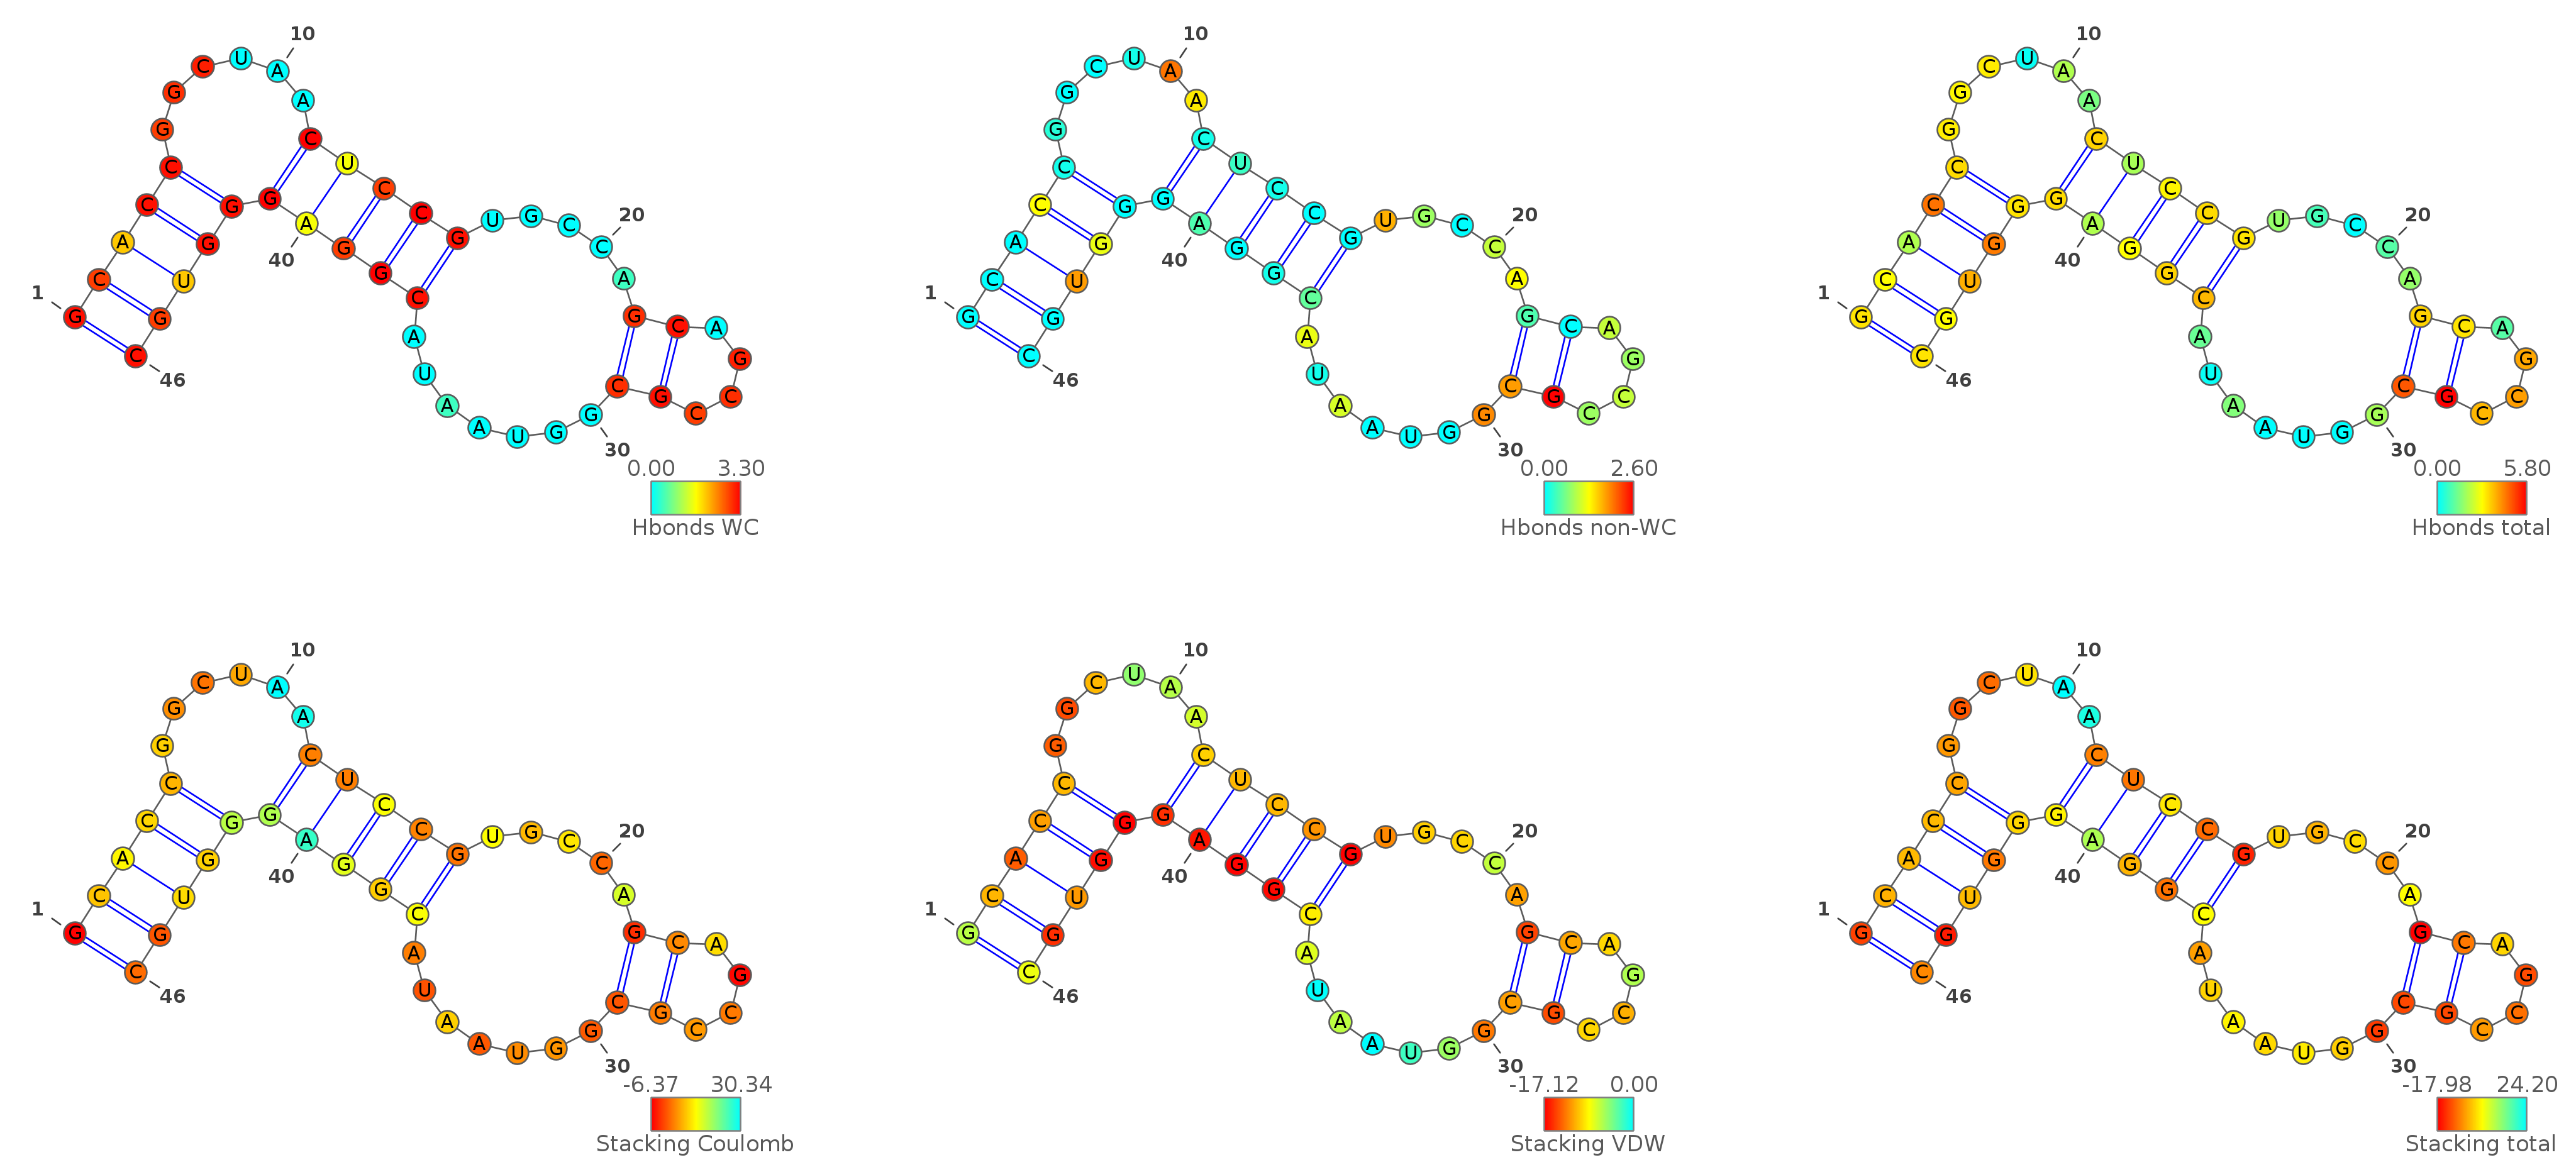
\includegraphics[scale=0.5]{./pictures/varna6.png}
\caption{Figures with average secondary structure colored by the values of computed parameters, generated by {\tt MINT} and displayed with the VARNA \cite{Blin2009} program, respectively: number of WC hydrogen bonds, number of non-WC hydrogen bonds, total number of hydrogen bonds, Coulomb therm of Stacking energy in kcal/mol, Van der Waals term of Stacking energy in kcal/mol, sum of the Coulomb and Van der Waals interactions in kcal/mol. In case of energy (Coulomb and VDW) the color scale is reversed so the red nucleotides are the ones that are influenced by the strongest hydrogen bonding and stacking interactions. }
\label{varna}
\end{figure}

\subsection{Inputs for external visualization tools} 
Files needed for visualization using external tools (see Section \ref{Visualization} for details):
\begin{itemize}
\item {\tt \_RNAStructML.xml} 
\item {\tt \_Hbonds-WC.pdb}
\item {\tt \_Hbonds-non-WC.pdb}
\item {\tt \_Hbonds-total.pdb}
\item {\tt \_Stacking-Coulomb.pdb}
\item {\tt \_Stacking-VDW.pdb}
\item {\tt \_stacking-total.pdb}
\item {\tt \_vmd\_run.tcl}
\end{itemize}


\section{Methods}
\subsection{Workflow}
Figure \ref{ProgramScheme} shows the structure of the program. First, the program reads in the conformation and finds all hydrogen bonds between nucleotides. Using that, it determines secondary, tertiary structures and subsequently classifies the secondary structural motifs. The main outcome is a set of statistical descriptors of the given RNA structure.  
\begin{figure}[hbt!]
\centering
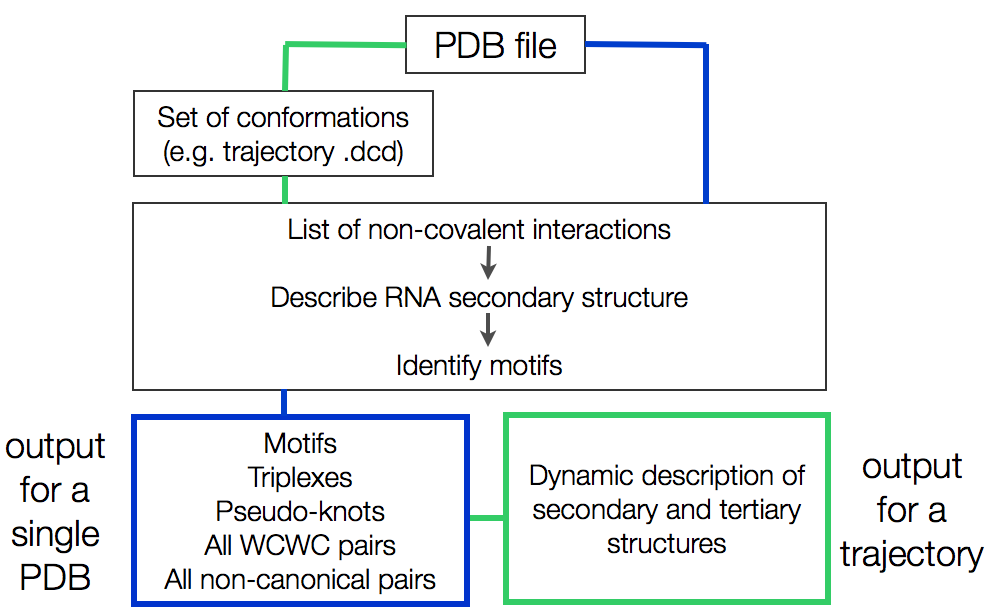
\includegraphics[scale=0.4]{./pictures/workflow.png}
\caption{Main function implements the analysis of a single frame. In the case of a trajectory, the function reads-in the list of nucleotides from a given PDB and then refreshes the atom coordinates while reading sequential frames. Additionally, the script splits the trajectory between CPUs and runs separate processes, what  accelerates the calculations.}
\label{ProgramScheme}
\end{figure}

\newpage
\subsection{Loading the DNA or RNA conformations}
All of the scripts are written in {\tt Python} programming language. Its modular structure enables applying it in various programming contexts. Reading the PDB file is implemented in {\tt BioPython} package, providing a complete objective structure for dealing with PDBs. 

In {\tt BioPython} an atom is a basic object with fields for a name, number and spatial coordinates. Atoms build residues and residues chains, chains molecules. This allows fast and easy access to the chains, nucleotides, atoms and finally their coordinates.

\subsection{Calculating physico-chemical features}
\subsubsection{Hydrogen bonding} \label{Hbond-section}
Hydrogen bonds are basic interactions responsible for creating the secondary and tertiary structures of nucleic acids. A typical definition of a hydrogen bond pertains to a non-covalent interaction when a hydrogen atom, covalently bound to its donor, is placed close to its acceptor.

Criteria for detecting hydrogen bonding is based on the angle, created by donor, hydrogen and acceptor, and distance between acceptor and hydrogen or between donor and acceptor (Figure \ref{hbond}). Theory states that all hydrogen bonds are almost linear (around $175^\circ$) \cite{Guerra2000}. For biological molecules the hydrogen bond distance should be typically between 2,80 and 3,06 \AA\ between a donor and acceptor, which gives 1,60 and 1,80 \AA\ between an acceptor and hydrogen. The user can decide which distance will be measured by {\tt MINT} using the {\tt h\_bond\_atom} parameter.

\begin{figure}[h!btp]
\centering
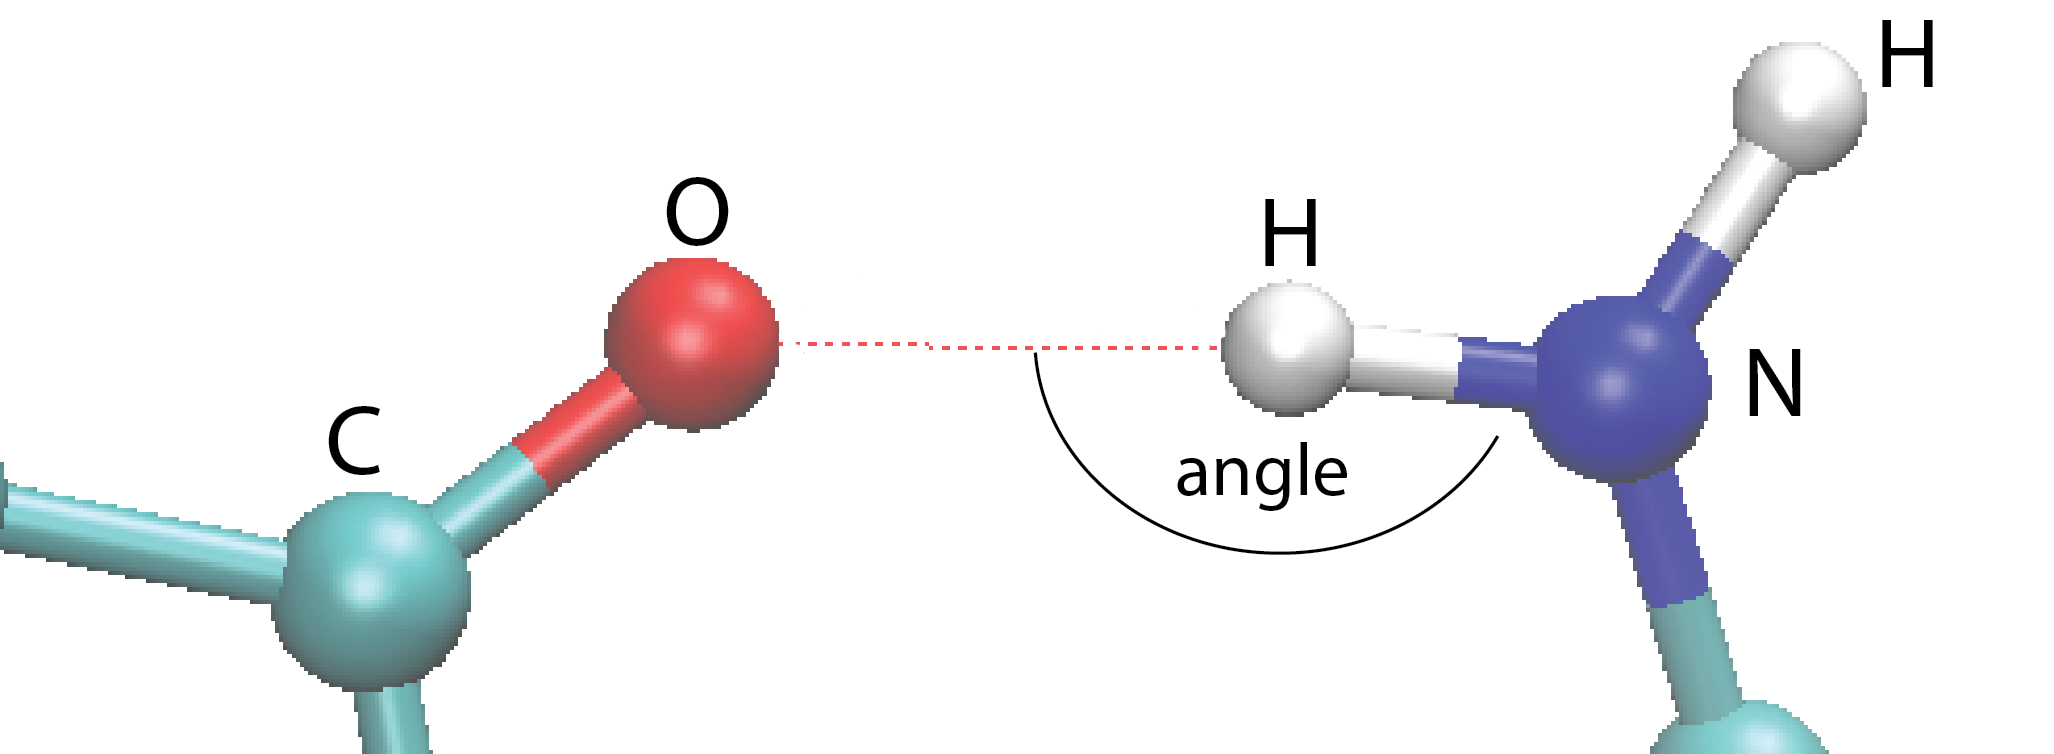
\includegraphics[width = 10cm]{./pictures/hydrogen_bond_2.png}
\caption{The scheme of the hydrogen bond with the nitrogen atom as a donor and the oxygen atom as an acceptor.}
\label{hbond}
\end{figure}

Other user defined parameters are: the minimal angle and the maximal length of a hydrogen bond. The default values of the {\tt h\_bond distance} (3.5 \AA) and the {\tt h\_bond\_angle} ($150^\circ$) are consistent with the distance calculated between donor and acceptor atoms.

It is possible that in the crystal structures or user-provided structures more than three hydrogen bonds in a GC pair (see Figure \ref{hbond4}) or two in AU pair will satisfy the above criteria. The user can remove the "unwanted" hydrogen bonds by decreasing the distance and/or increasing the angle. However, one should have in mind that too strict criteria can cause errors in the analysis of nucleotide pairs and assignment of the RNA secondary structure. 
\begin{figure}[h!btp]
\centering
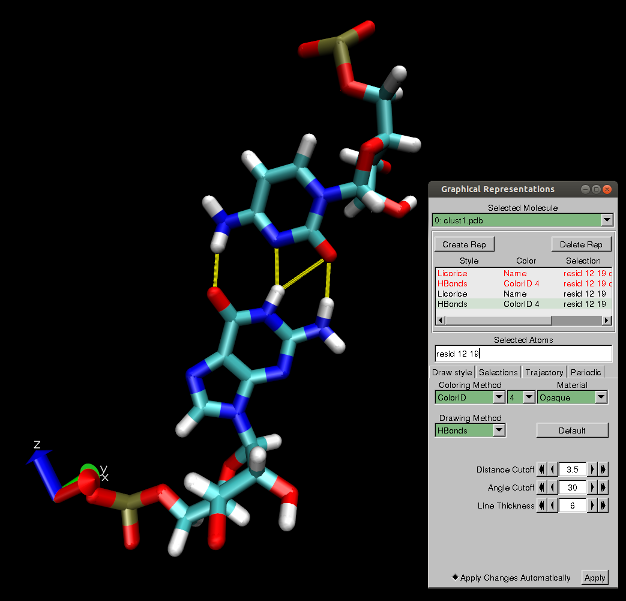
\includegraphics[width = 12cm]{./pictures/hbonds-GC-4.png}
\caption{Visualization of four possible hydrogen bonds (yellow) found in the GC pair using default parameters for hydrogen bonds.}
\label{hbond4}
\end{figure}


\subsubsection{Donors and acceptors} \label{donrsandacceptors}
To analyze the structures we have defined a list of possible acceptors and donors for all nucleotides of RNA and DNA. Following the classification by Leontis and Westhof \cite{Leontis2002} the acceptors and donors are assigned to the edges of the nucleotide (Figure \ref{Edges}). This classification is stored in the {\tt table\_nucleotides} .csv file and may be edited by the user. 

{\tt MINT} determines the interacting edges of every pair of nucleotides. Several atoms are situated in the corners of the nucleotides and participate in more than one edge. In that case, the program first classifies all the remaining bonds and chooses the prevailing edge. If there is only one hydrogen bond, both edge names are returned. 

\begin{figure}[h!]
\centering
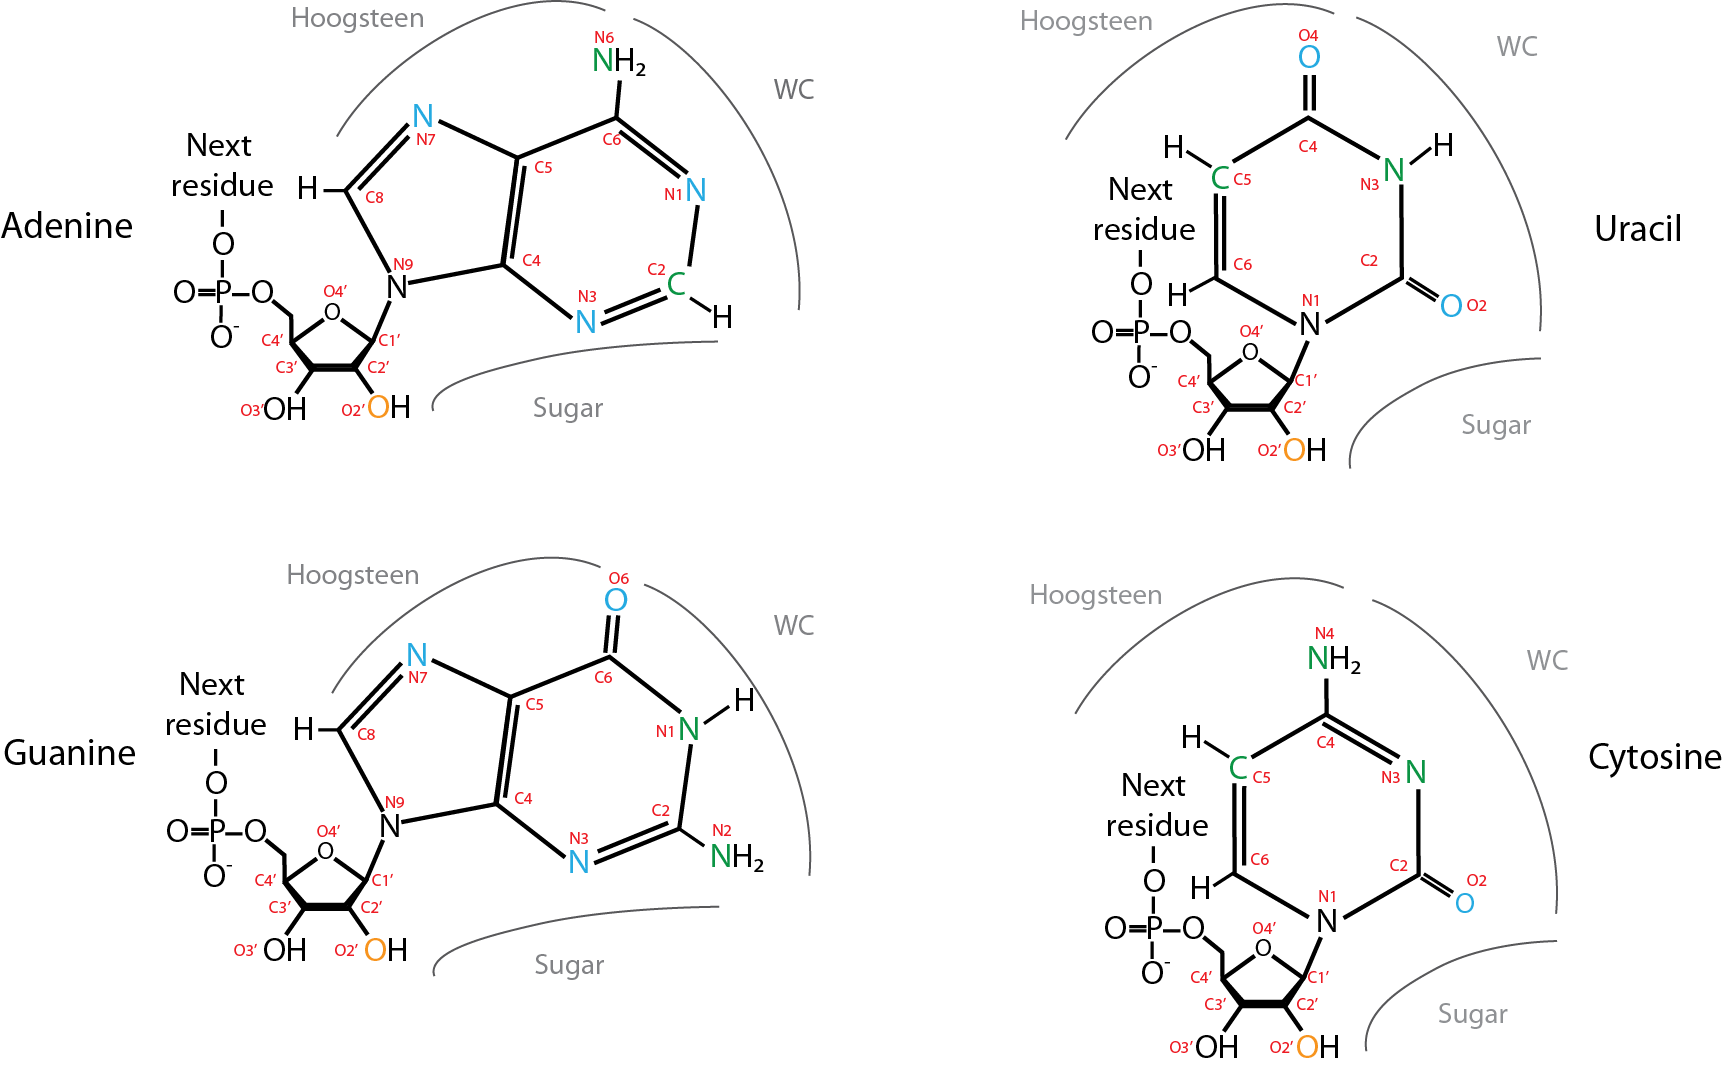
\includegraphics[width = 14cm]{./pictures/donors_acceptors_nucleotides.png}
\caption{Nucleotides with selected edges, donors (green) and acceptors (blue). WC corresponds to WC edge.  \cite{Lescoute2006}.}
\label{Edges}
\end{figure}

% Pairs
{\tt MINT} checks all the donors against all acceptors in all possible pairs of all nucleotides in the molecule. In order to decrease the computational time, we assume that the partner for a given nucleotide can be found only among its closest neighbors. The exact distance is defined by the user in the {\tt cutoff} parameter. Knowing the atoms creating hydrogen bonds, the program  determines the interacting edges and classify the basepair.

Note that we use the edge-to-edge classification, instead of the concept of the canonical base pairs, to unambiguously and consistently describe all possible geometric pairs that may, even transiently, occur in a trajectory.
The pair is classified as WC-WC if both nucleotides make hydrogen bonds with the WC edges. If there is only one bond between the nucleotides, the pair will be classified as WC-WC only if edges in both nucleotides can be unambigously diefined. For example if at least one of the interacting atoms is located on the "corner" between two edges (see: \ref{Edges}) the pair will be classified as non-WC-WC. If there are more than one hydrogen bonds between nucleotides than the edges are clearly defined and pair classification is straighforward. 


\subsubsection{Modified nucleotides}
Modified nucleotides are found in almost all RNAs and are believed to be functionally important, for example, in tRNAs. A few modified nucleotides are presented in Figure \ref{ModifiedNucleotides}. 
\begin{figure}[h!]
\centering
\begin{center}
\subfigure[2MG]{
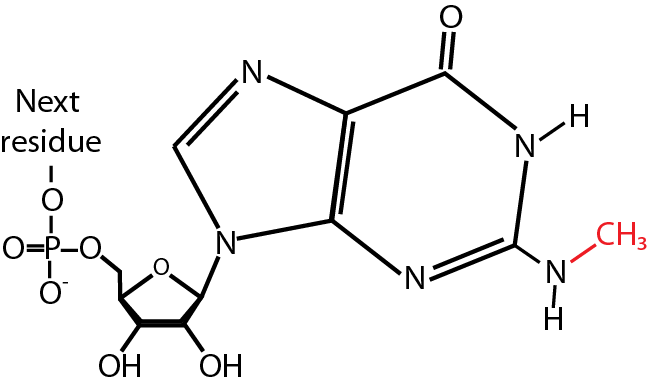
\includegraphics[scale=0.8]{./pictures/modified_1.png}}
\subfigure[OMC]{
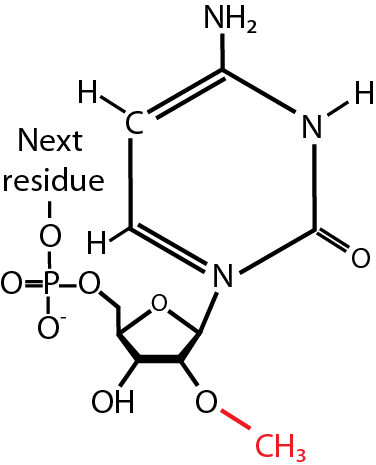
\includegraphics[scale=0.8]{./pictures/modified_2.png}}
\subfigure[YYG]{
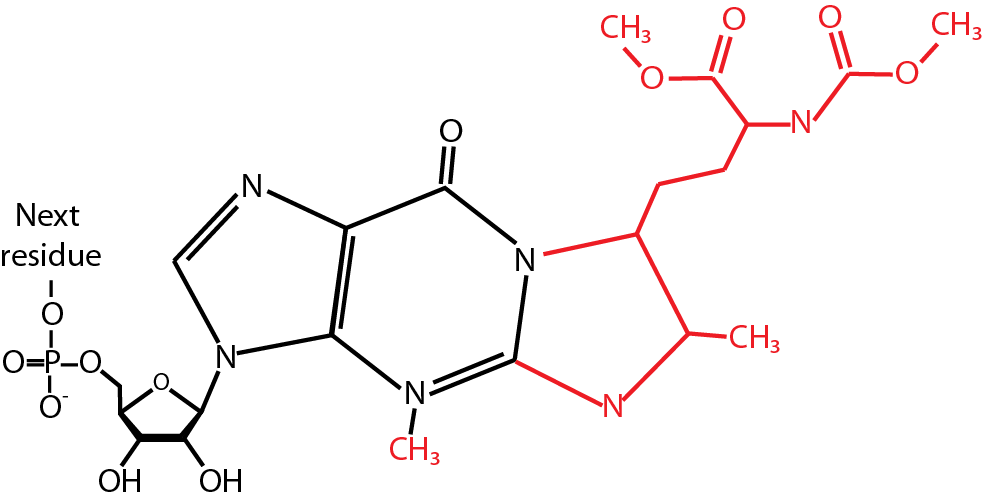
\includegraphics[scale=0.8]{./pictures/modified_3.png}}
\end{center}
\caption{Three out of ten modified nucleotides present in the structure of tRNA (PDB code: 1TTT) along with their PDB names. The atoms that are not present in standard nucleotides are shown in red.}
\label{ModifiedNucleotides}
\end{figure}

There are about 600 modified RNA nucleotides in the PDB database, but for most of them there are no force field parameters. With {\tt MINT} we provide the VDW parameters and partial atomic charges for 107 naturally occurring modified nucleotides whose force fields were developed by Aduri et al~\cite{Aduri_2007}. For these nucleotides, we have also assigned their atoms to distinct edges: the WC edge, the Hoogsteen edge, the sugar edge and to the edge termed the modification edge (see Section \ref{donrsandacceptors} for details about the classification of edges). 

An atom in a modified nucleotide, common to the unmodified one, is assigned into the same edge as in the unmodified nucleotide. The addition of no more than one heavy atom to the nitrogenous base is also classified into the same edge as the base atom. The 2'O methyl carbon is assigned to the sugar edge. All other atoms present in the modified nucleotide but not in the original one are assigned to the modification edge.

If {\tt MINT} encounters a modified nucleotide, it looks for its parameters in the {\tt table\_nucleotides}. If parameters are not found, {\tt MINT} uses the {\tt list\_of\_modified\_nucs} to find the natural ancestor of the modification. Atoms common to the modified and its natural ancestor are assigned analogously as in the original nucleotide, the rest is assigned to the modification edge. If there are no partial charges and VDW parameters, the stacking interaction energy is set to 0.

However, the user can add new modified nucleotides. The force field parameters developed for a modified nucleotide for an MD simulation, can be adopted to the {\tt MINT} parameter format. If you want to add your own modification to the {\tt MINT} parameters: you should edit the {\tt table\_nucleotides} file and add a new row with the name of your residue and appropriate names of atoms in the donor and acceptor columns. Next, you should also modify the {\tt table\_charges} file. For every atom that should be considered in stacking computation you have to add a row with the name of the residue, charge, VDW radius and well depth parameter. For details see Sections \ref{Hbond-section} and~\ref{stacking-section}.

\subsubsection{Geometric isomerism of base pairs}
For detected base pairs the geometric isomerism of their glycosidic bonds is computed. The program measures the torsion angle formed by the four atoms (C1', N1 in pyrimidines and C1', N9 in purines) and depending on its value a {\it cis} or {\it trans} conformation is denoted (see Figure \ref{Conf}).

\begin{figure}[h!]
\begin{center}
\subfigure[Cis]{
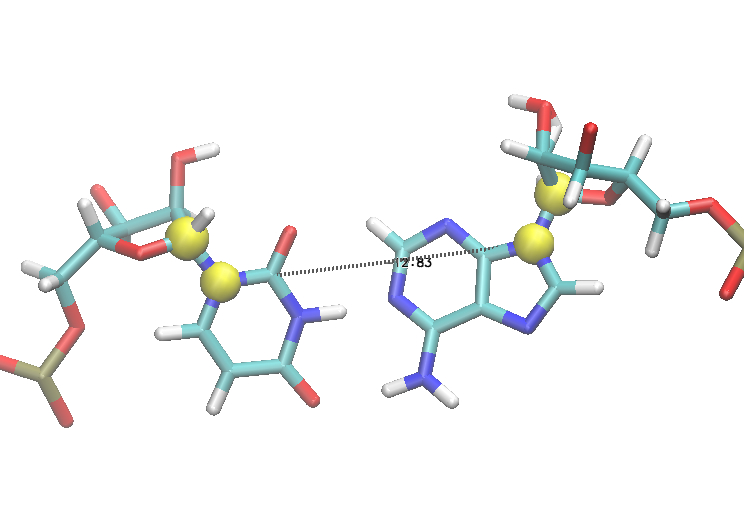
\includegraphics[width=6.5cm]{./pictures/torsion_angle_cis.jpg}}
\subfigure[Trans]{
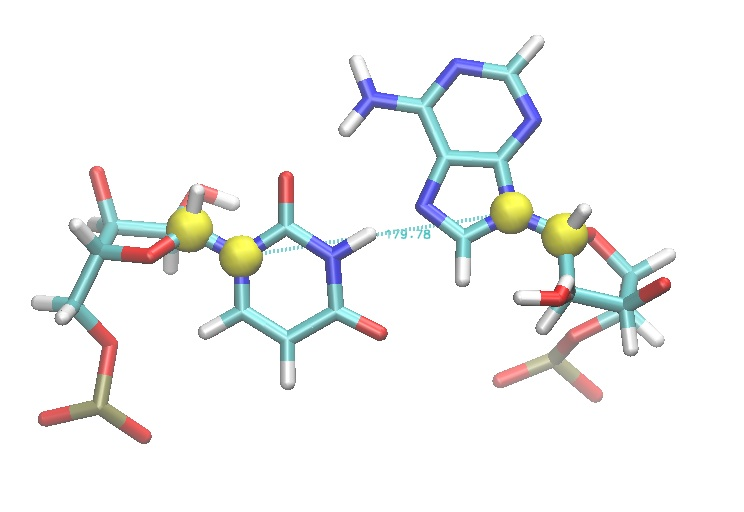
\includegraphics[width=6.5cm]{./pictures/torsion_angle_trans.jpg}}
\end{center}
\caption{Yellow spheres correspond to C1' and N1 atoms in pyrimidines and N9 atoms in purines. The torsion angle created by these four points determines the geometric isomerism of the two nucleotides creating a pair. }
\label{Conf}
\end{figure}

%Stacking interactions
\subsubsection{Stacking}
\label{stacking-section}
Stacking is an important non-covalent interaction contributing to the stability of both double helix and single stranded structures of nucleic acids \cite{Hobza2008}. For instance, in tRNA only half of the nucleotides form a helix but about 90\% are stabilized by stacking \cite{Bloomfield1999}. 
\begin{figure} [h!]
\begin{center}
\subfigure[]{
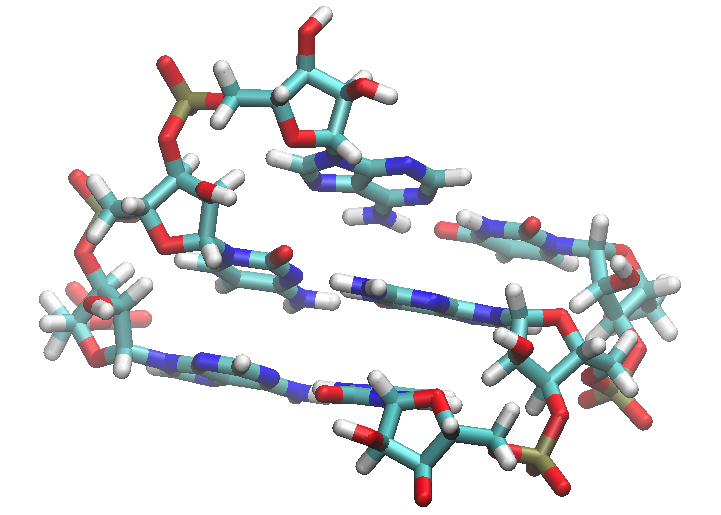
\includegraphics[width=5.0cm]{pictures/stacking1.png}}
\subfigure[]{
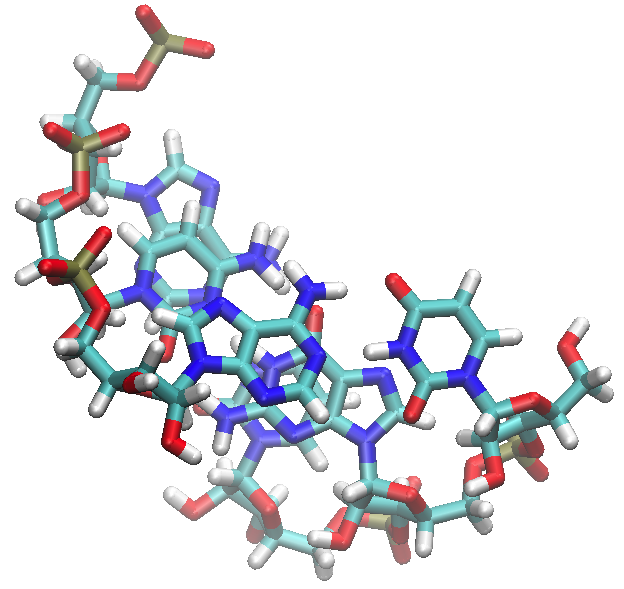
\includegraphics[width=5.0cm]{pictures/stacking2.png}}
\subfigure[]{
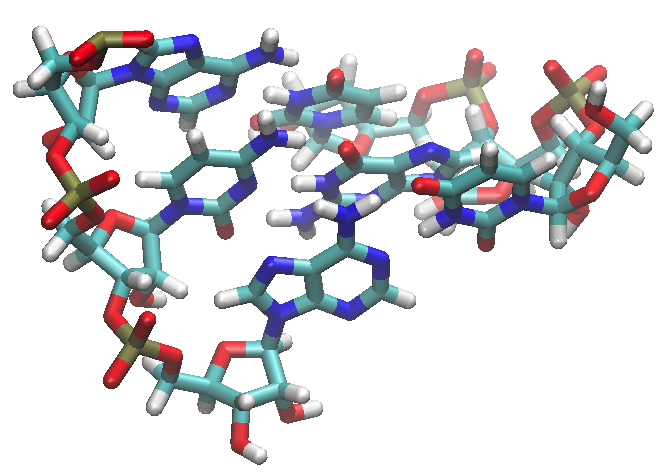
\includegraphics[width=5.0cm]{pictures/stacking3.png}}
\caption{Three-pairs of an RNA helix seen from different angles to expose  stacking between parallel bases.}
\label{StackingHelix}
\end{center}
\end{figure} 
Generally, stacking occurs between aromatic rings so in nucleic acids between the nucleobases. There is a general belief that stacking results from the contact of the electron $\pi$-systems. Stacking also arises from three phenomena: Van der Waals (dipole or induced-dipole attractions), electrostatic and solvation effects. Stacking interactions seem to be more important in folding of nucleic acids than proteins because nucleobases are more polarizable than most amino-acids. 

%In order to measure stacking separately of hydrogen bonding the experiments where conducted with a helix terminated with a single nucleotide. Presence of the unpaired nucleotide  stabilizes the entire helix. Sites are uneven, for DNA the on the $5\prime$ site of the helix is more favorable energetically than the other one, but for RNA the $3\prime$ is \cite{Kool2001}. Experimental studies indicated ability of stacking among natural bases is the strongest between two purines, than purine-pyrimidine and pyrimidine-pyrimidine \cite{Guckian2010}.

Stacking is believed to be represented well in molecular modeling, especially with the Amber atomic charges which are fitted to molecular electrostatic potentials~\cite{Hobza2008}. It was shown that calculations using the empirical potentials consisting of the Lennard-Jones VDW and Coulombic terms with atom-centered point charges reproduced the {\it ab initio} stacking energy over the major portion of the conformational space~\cite{Leszczynski2002}.
\v{S}poner et al. in many studies~\cite{Carter2000,Sponer1997, Base1996, Hobza1995} compared {\it ab initio} energies for about 300 geometries of stacked base dimers with the data obtained using empirical potentials. The agreement between these methods is remarkable, which suggests that calculations based on empirical potentials provide an excellent approximation of the stacking interaction energy between nucleotides. Therefore, {\tt MINT} calculates the stacking interactions.

We estimate stacking between two bases by calculating the energy of electrostatic ($U_{el}$) and Van der Waals ($U_{VDW}$) interactions applying the equations used in molecular mechanics:
\begin{equation}
U_{el} = k \sum{\frac{q_i q_j}{r_{ij}}}
\end{equation}

\begin{equation}
U_{VDW} = 4 \epsilon_{ij} \sum{ \left[ \frac{1}{4} {\left( \frac{r_0}{r_{ij}} \right) }^{12} - \frac{1}{2} {\left( \frac{r_0}{r_{ij}} \right) }^{6} \right]}
\end{equation}
The sums run over all atom pairs of nucleobases $i$ and $j$, $k$ denotes the Coulomb constant ($k = \frac{1}{4 \Pi \epsilon_0}$), $q$ is the partial atomic charge of the atom, $r_{ij}$ is the distance between the considered atoms, $\epsilon_{ij}$ is the depth of the Lennard-Jones potential well for atoms $i$, $j$ ($\epsilon_{ij} = \sqrt{\epsilon_{ii}\epsilon_{jj}} $) and $r_0$ is the sum of VDW radii of atoms $i$ and $j$. We provide the VDW well depth parameters and partial atomic charges from the Amber~\cite{Wang2000} and Charmm~\cite{Mackerell2000,Foloppe2000} force fields. A set of parameters and charges may be also defined by the user in the file {\tt table\_charges} file. Only the nucleobases that are closer than the user defined cutoff ({\tt cutoff\_stacking}) are considered in the stacking calculations. The energy unit obtained from described calculations is $kcal/mol$. 

The electrostatic term, depending on the orientation of base dipole moments, may be attractive or repulsive regardless of the mutual orientation of the bases (parallel or not). While the VDW energy component is almost always favorable regardless of the orientation of bases. Moreover, the shape of nucleotides and the method used for calculating the VDW energy ensure that the lowest VDW energy values are obtained for the parallel orientation of nucleobases (with their largest overlap). This was also the case in our test calculations. Thus we recognize two nucleotides as stacked, if their VDW energy is lower than the {\tt vdw\_cutoff\_stacking} parameter. The default value of this parameter is $ -0.5 kcal/mol$ which was found by trial and error and seems appropriate for the nonmodified nucleobases.

%\subsection{Anion-$\pi$ contacts} Following recent research on the types of non-covalent contacts in RNA molecules, {\tt MINT} also analyzes the anion-$\pi$ - contacts and hydrogen bonding interactions, per nucleotides and in pairs \cite{Auffinger2013}. Detection of these interactions is based on the distance between the oxygen atom and the center of the mass of a nucleobase ring. 

\subsubsection{Ion-$\Pi$ interaction between a nucleobase and phosphate oxygen}
Hydrogen bonds are the most known non-covalent interactions but are not the only one. For example, the cation-$\Pi$ interactions, namely the non-covalent bonding between a monopole (cation) and a quadrupole ($\Pi$ system), play a role in the structure of proteins. A similar interaction was reported for RNA but it was found that nucleic acid aromatic systems prefer to interact with anionic rather than cationic species~\cite{Auffinger2013}. 
{\tt MINT} enables searching for anion-$\Pi$ interactions involving the RNA backbone phosphate groups and nucleobases. An example of such a contact is shown in Figure \ref{stackingPiExamples}.
\begin{figure}[h!]
\begin{center}
\subfigure[]{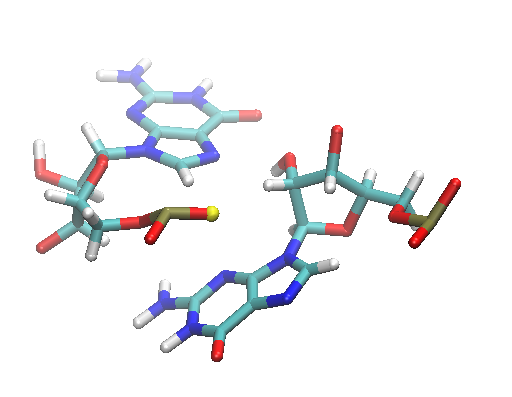
\includegraphics[scale = 0.3]{pictures/stacking_pi_1.png}
\label{stackingPiexample1}}
\subfigure[]{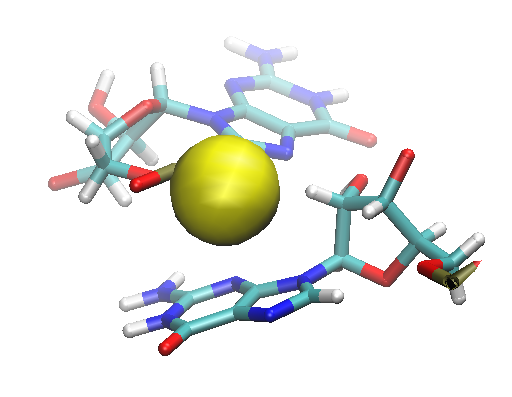
\includegraphics[scale = 0.3]{pictures/stacking_pi_2.png}
\label{stackingPiexample2}}
\subfigure[]{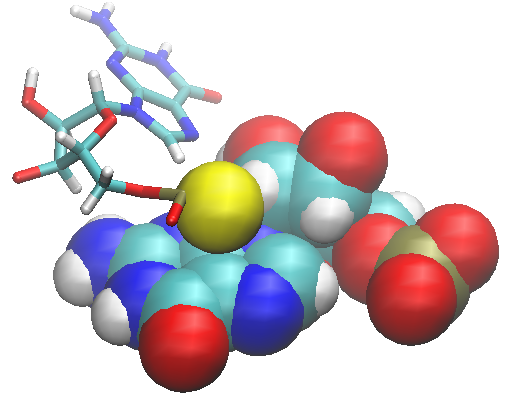
\includegraphics[scale = 0.3]{pictures/stacking_pi_3.png}
\label{stackingPiexample3}}
\caption{Three representations of the oxygen atom (yellow) "stacking" over the guanine base. The yellow sphere in the \label{stackingPiexample1} picture corresponds to the real VDW radius.}
\label{stackingPiExamples}
\end{center}
\end{figure}
The interacting systems are recognized if the distance between a phosphate atom and nucleotide base center of mass is lower than the {\tt OP\_stacking\_distance\_cutoff} parameter (default distance is $ 5 \AA$). If the ion-$\Pi$ stacking is detected, the energy of interaction between the phosphate atom and nucleobase is calculated in the same way as for the stacking between two nucleobases. 

\subsubsection{Representation of RNA motifs}
Having all WC pairs, a list-representation of the RNA secondary structure is created. 
Most nucleotides have only one WC-edge partner but in MD trajectory it may transiently happen that a second WC-edge partner is encountered, and such a triple is not considered in the secondary structure analysis. 
The index of the list represents the nucleotide number and the stored value is the index of its WC partner. The list is easy-interpretable when the arcs connecting the pairs are drawn as  presented in Figure \ref{SecondaryStructureList}. 

\begin{figure}[h!]
\centering
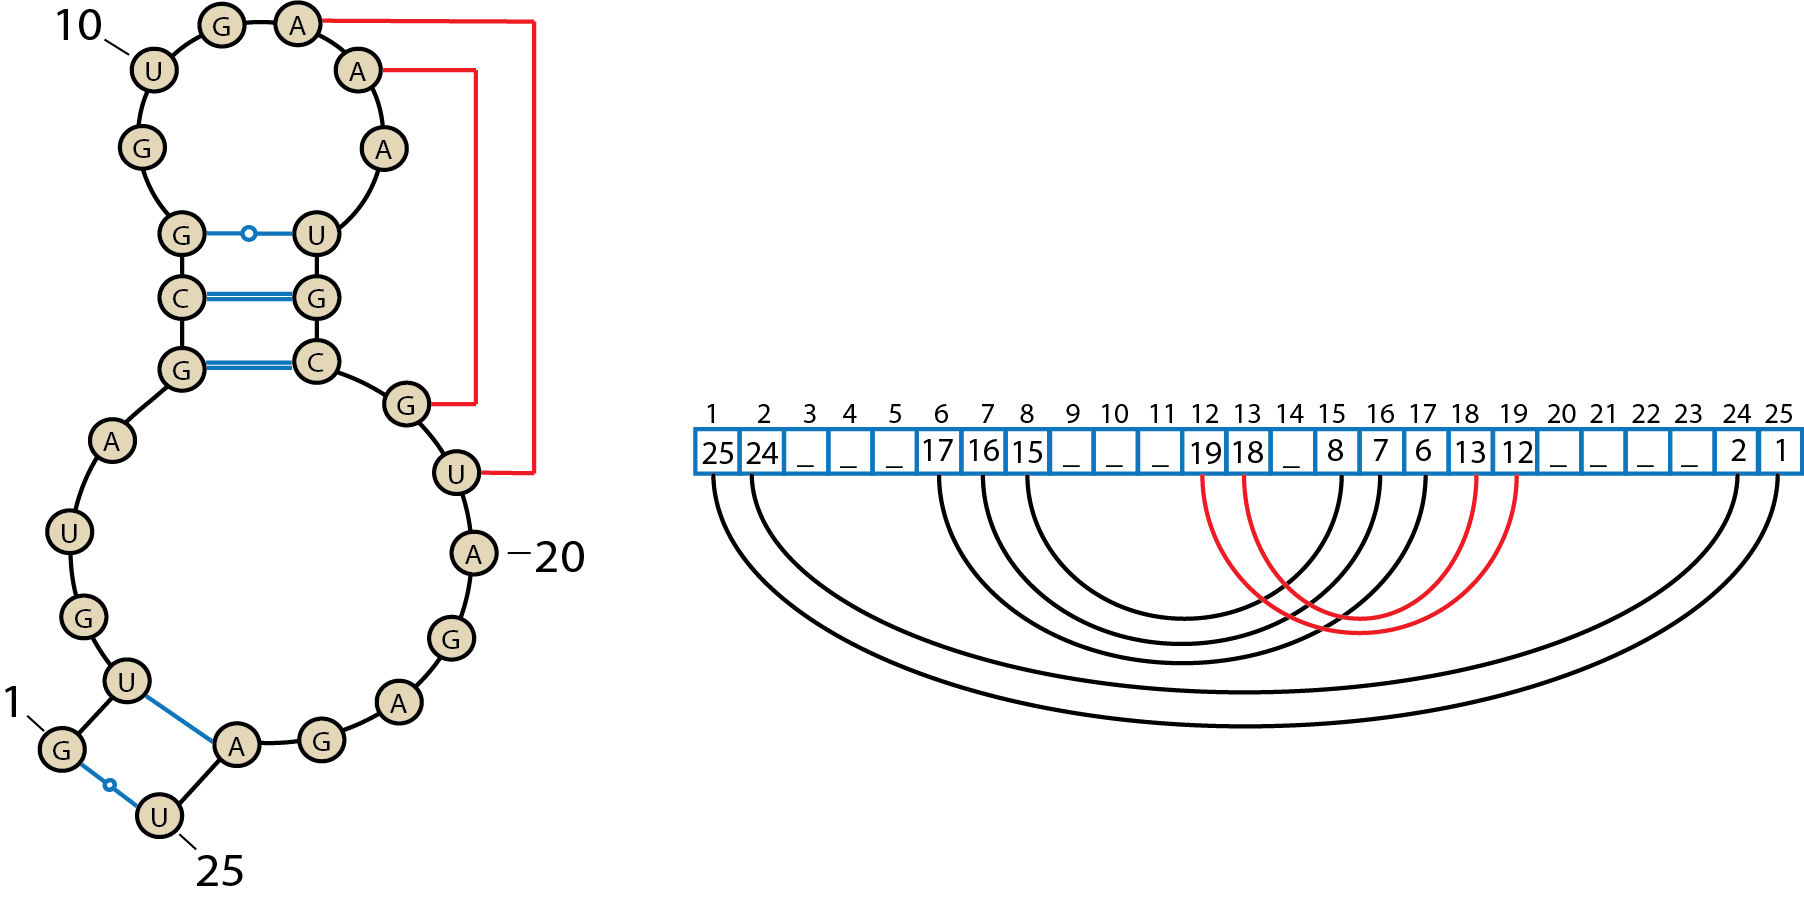
\includegraphics[width = \textwidth]{./pictures/PseudoKnotArchs.png}
\caption{Secondary structure of an exemplary RNA molecule and its list-representation. Red lines correspond to the WC interactions creating a pseudoknot.}
\label{SecondaryStructureList}
\end{figure}

\paragraph{Pseudo knots}
The list-representation contains also the information about the non-secondary motifs. The pseudoknot is formed by the WC interactions but creates three-dimensional folds as shown in Figure \ref{PseudoKnot}. Our program detects the pseudoknot fold when the arcs intersect. A pseudoknot is a symmetric structure so both the pairs 6--17, 7--16, 8--15 and 12--19, 13--18 in Figure \ref{SecondaryStructureList} form a pseudoknot. 
The natural way of solving this conflict is to choose the shorter list, in this case the pairs 12--19 and 13--18.
To erase pseudo-knots from the list-representation of the
secondary structure, so they do not disturb the motif-search
algorithm, we use a conflict elimination method~\cite{Smit_2008} leading
to a nested structure containing the maximum number of base
pairs.
  
\begin{figure}[h!]
\begin{center}
\subfigure[Tertiary structure]{
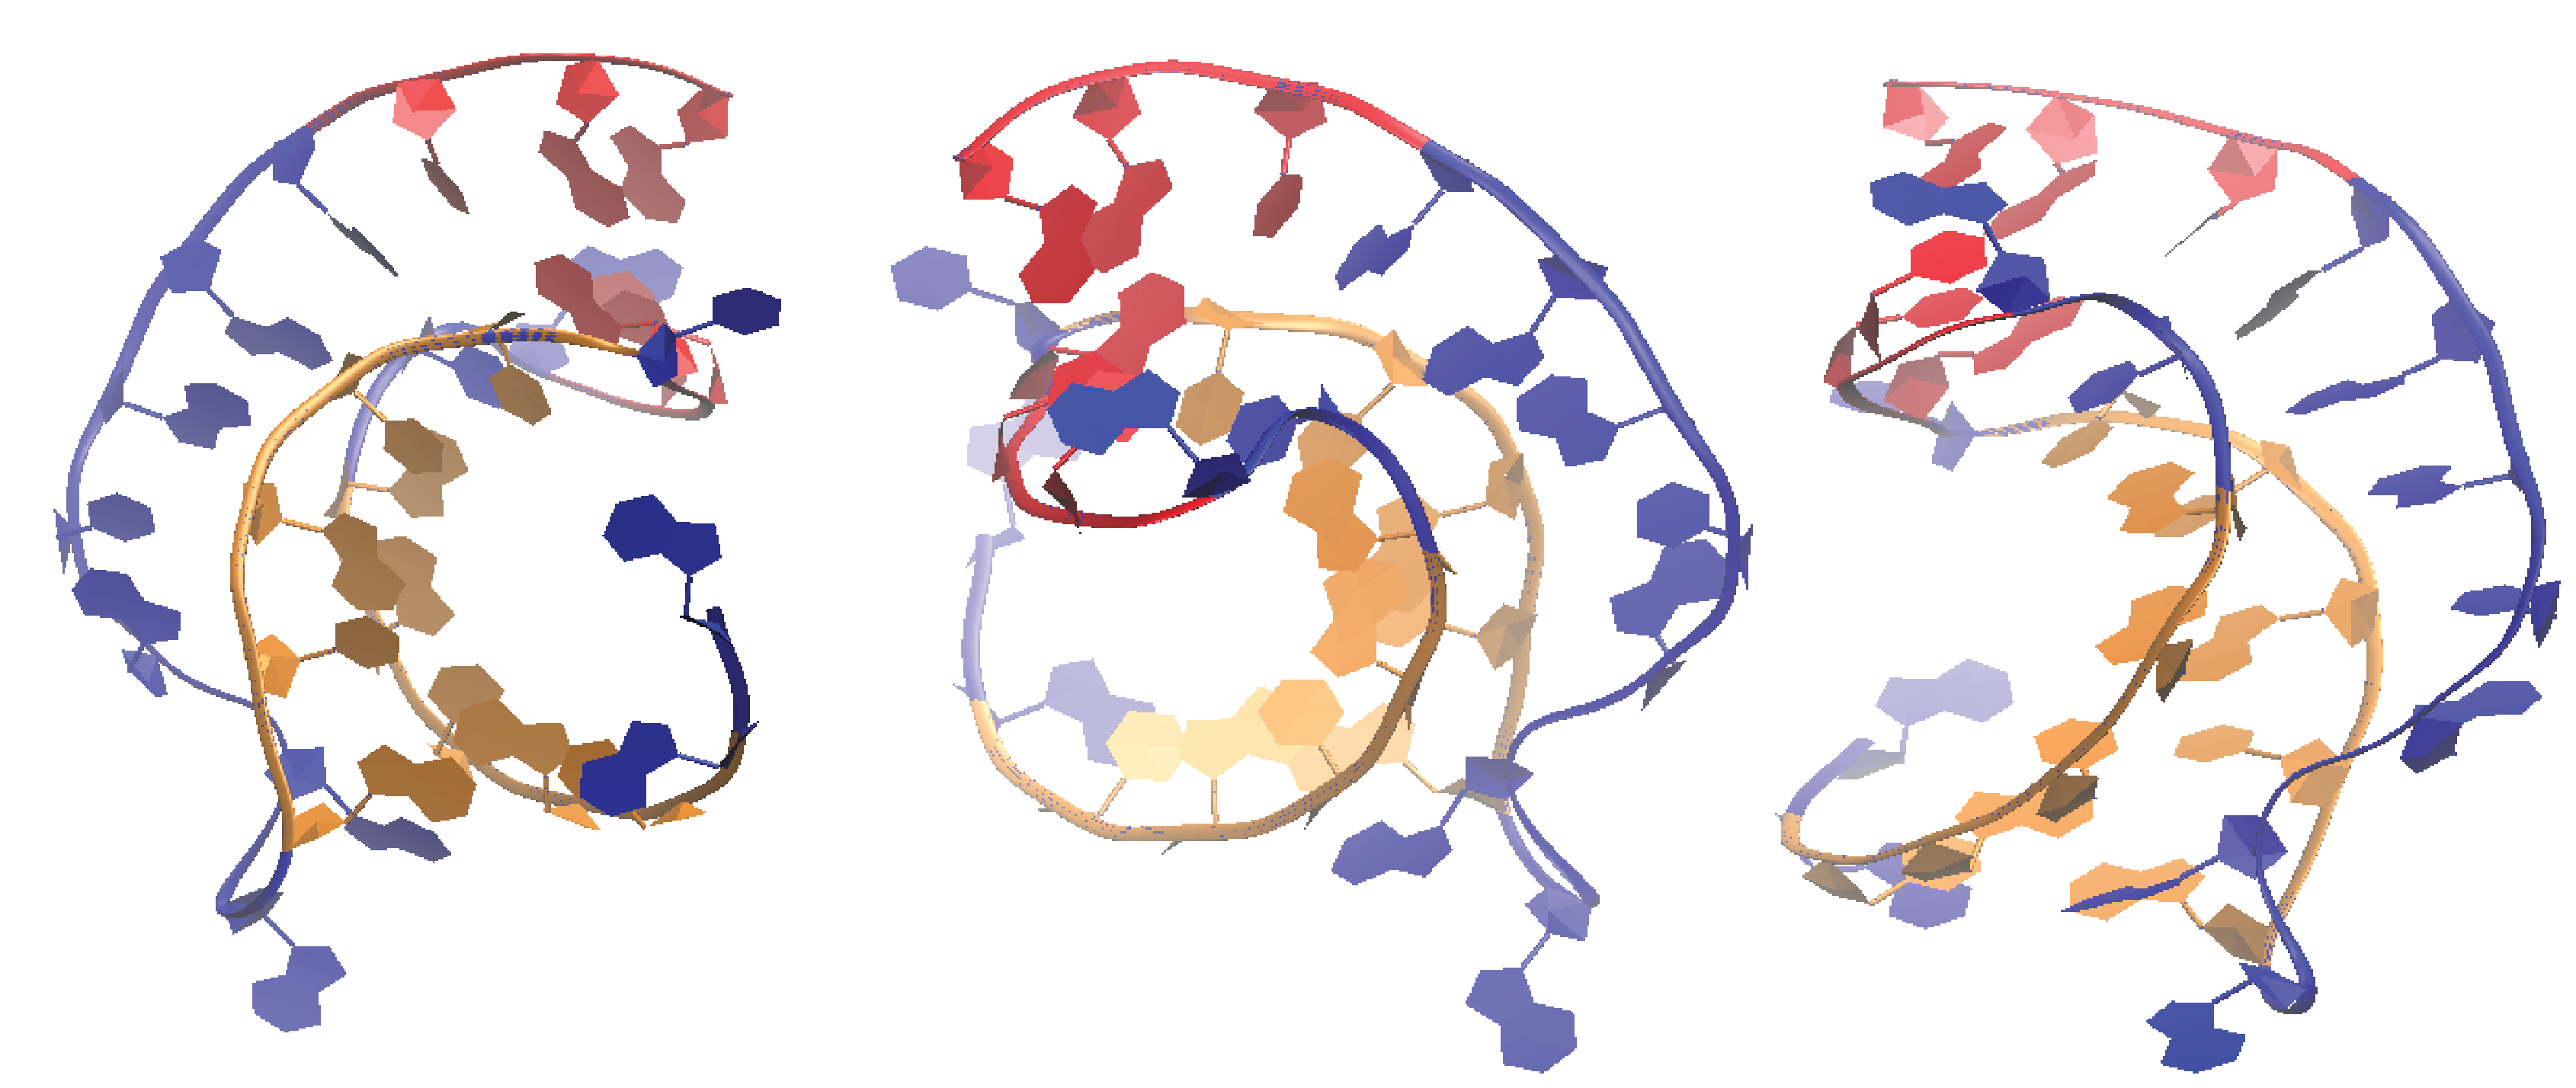
\includegraphics[width=12.5cm]{./pictures/pseudo_knot_combo.png}}
\subfigure[Secondary structure]{
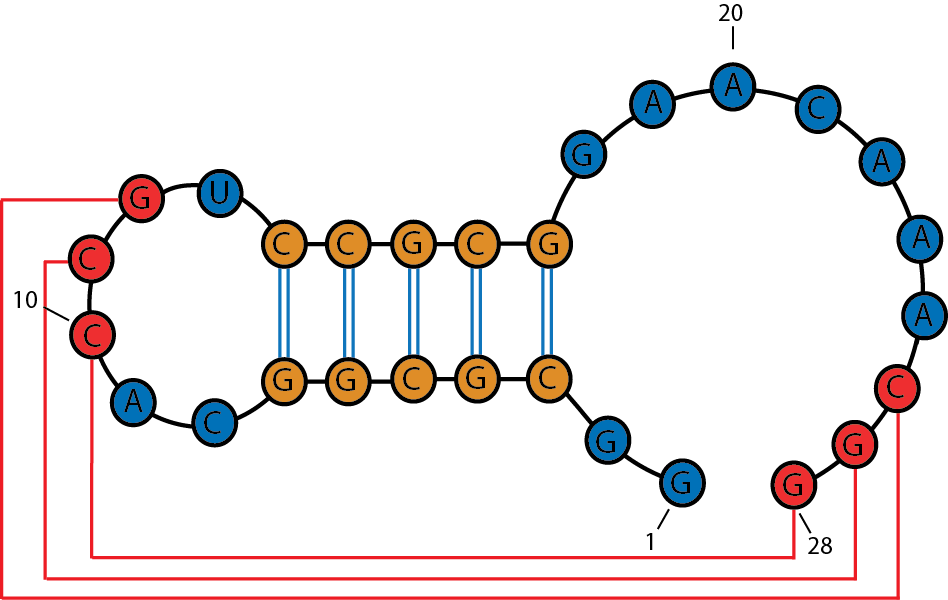
\includegraphics[width=6cm]{./pictures/pseudo_secondary_structure.png}}
\end{center}
\caption{An example of the RNA structure with a pseudoknot seen from three different angles. Nucleotides colored in red create a pseudoknot, orange form a helix and blue refer to loops (PDB code: 437d).}
\label{PseudoKnot}
\end{figure}
\newpage

After detecting all pairs and creating a list, {\tt MINT} finds all pseudoknots and erases them from the list by putting the {\tt None} value. Next, it looks for all other kinds of motifs, that are defined as a set of unpaired nucleotides surrounding the paired nucleotides as shown in Figure \ref{MotifDesc}.

\begin{figure}[h!]
\centering
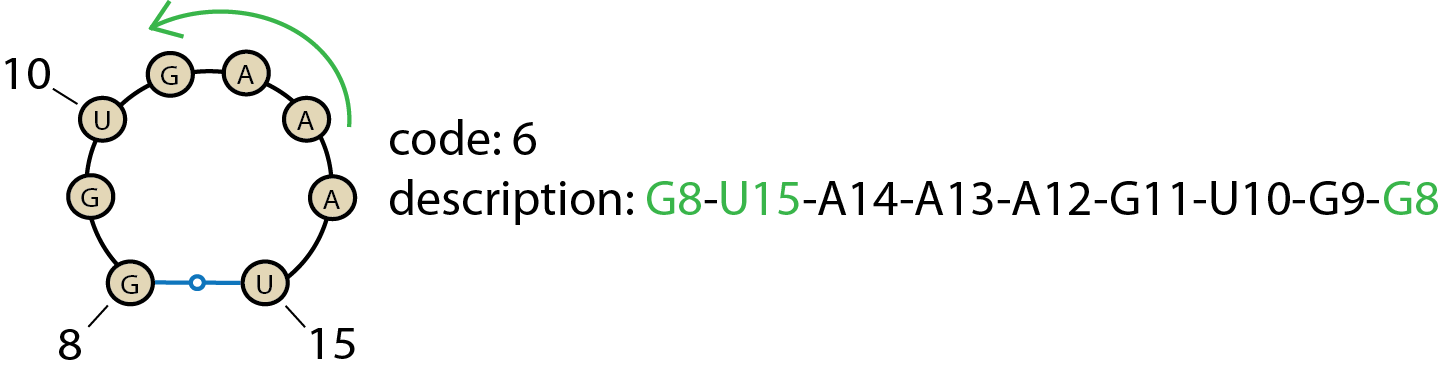
\includegraphics[width = \textwidth]{./pictures/motifs_description.png}
\caption{The program denotes the first pair (shown in green) and then makes a list of unpaired nucleotides. Nucleotides are listed in the counter-clockwise direction.}
\label{MotifDesc}
\end{figure}

\begin{table}
\caption{RNA secondary structure motifs}
\label{RNAsecondaryStructures}
\begin{tabular}
{ >{\centering} p{5.5cm} >{\centering} p{5.5cm} >{\centering} p{5.5cm}}
&& \tabularnewline
 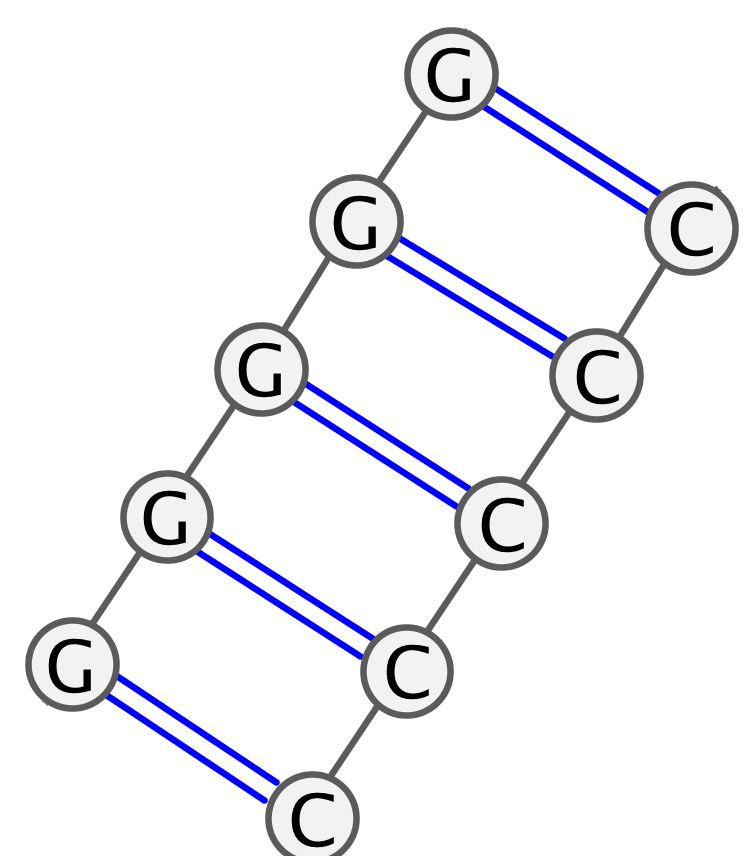
\includegraphics[width=4.5cm]{./pictures/helix_varna.PNG}  \linebreak Helix 
 & 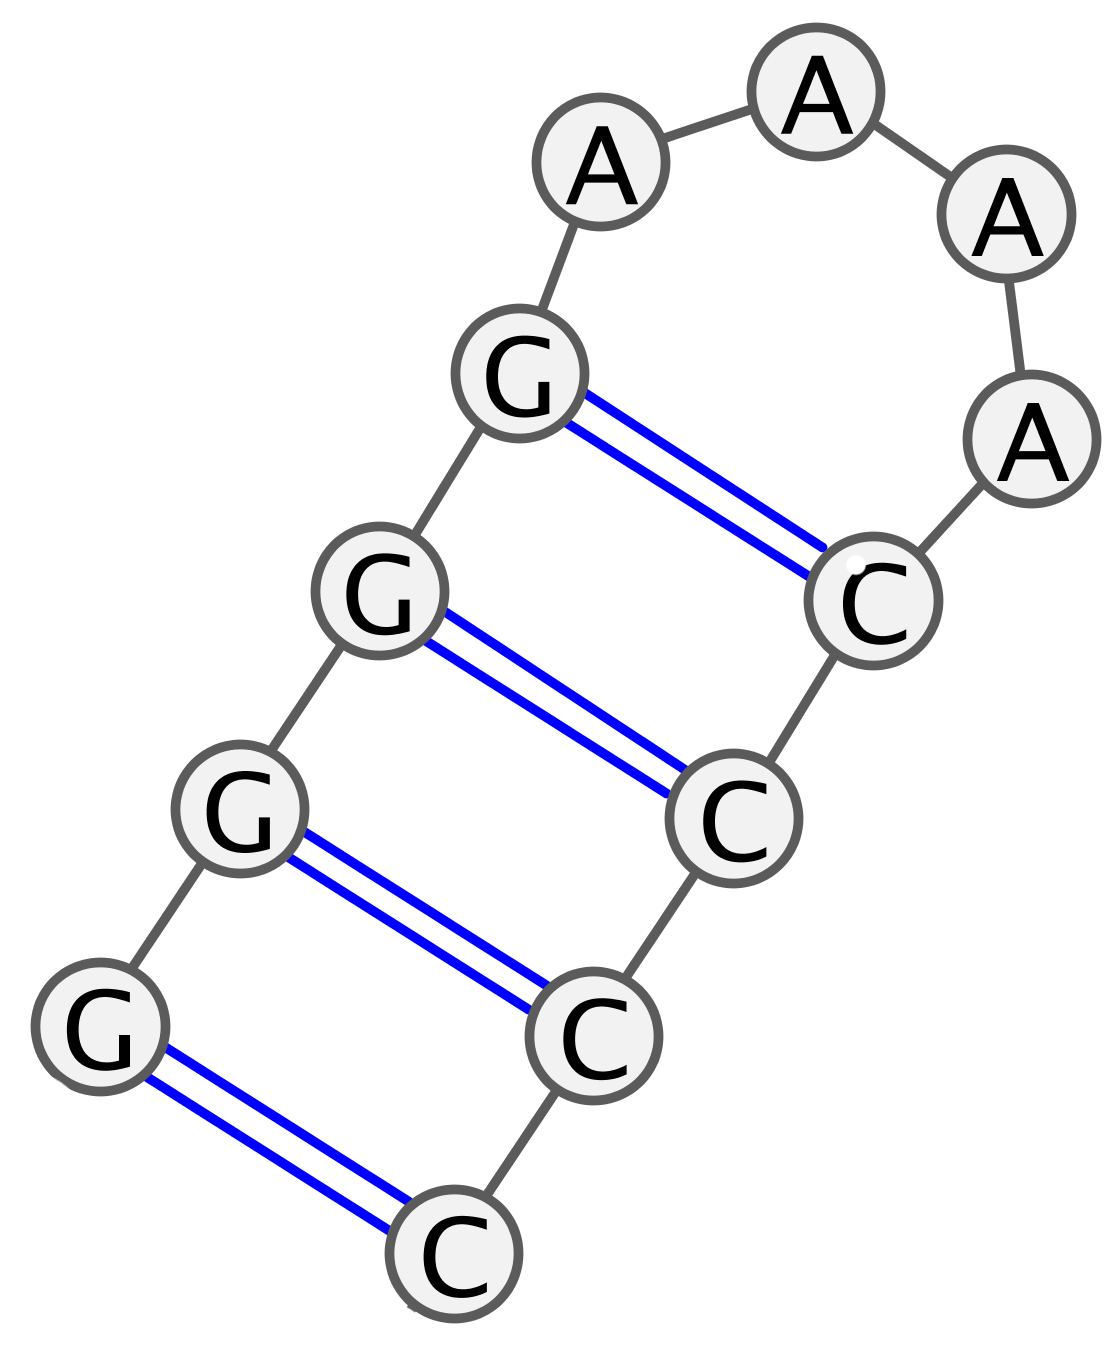
\includegraphics[width=4.5cm]{./pictures/hairpin_varna.PNG}  Hairpin loop \linebreak (code: 4) &  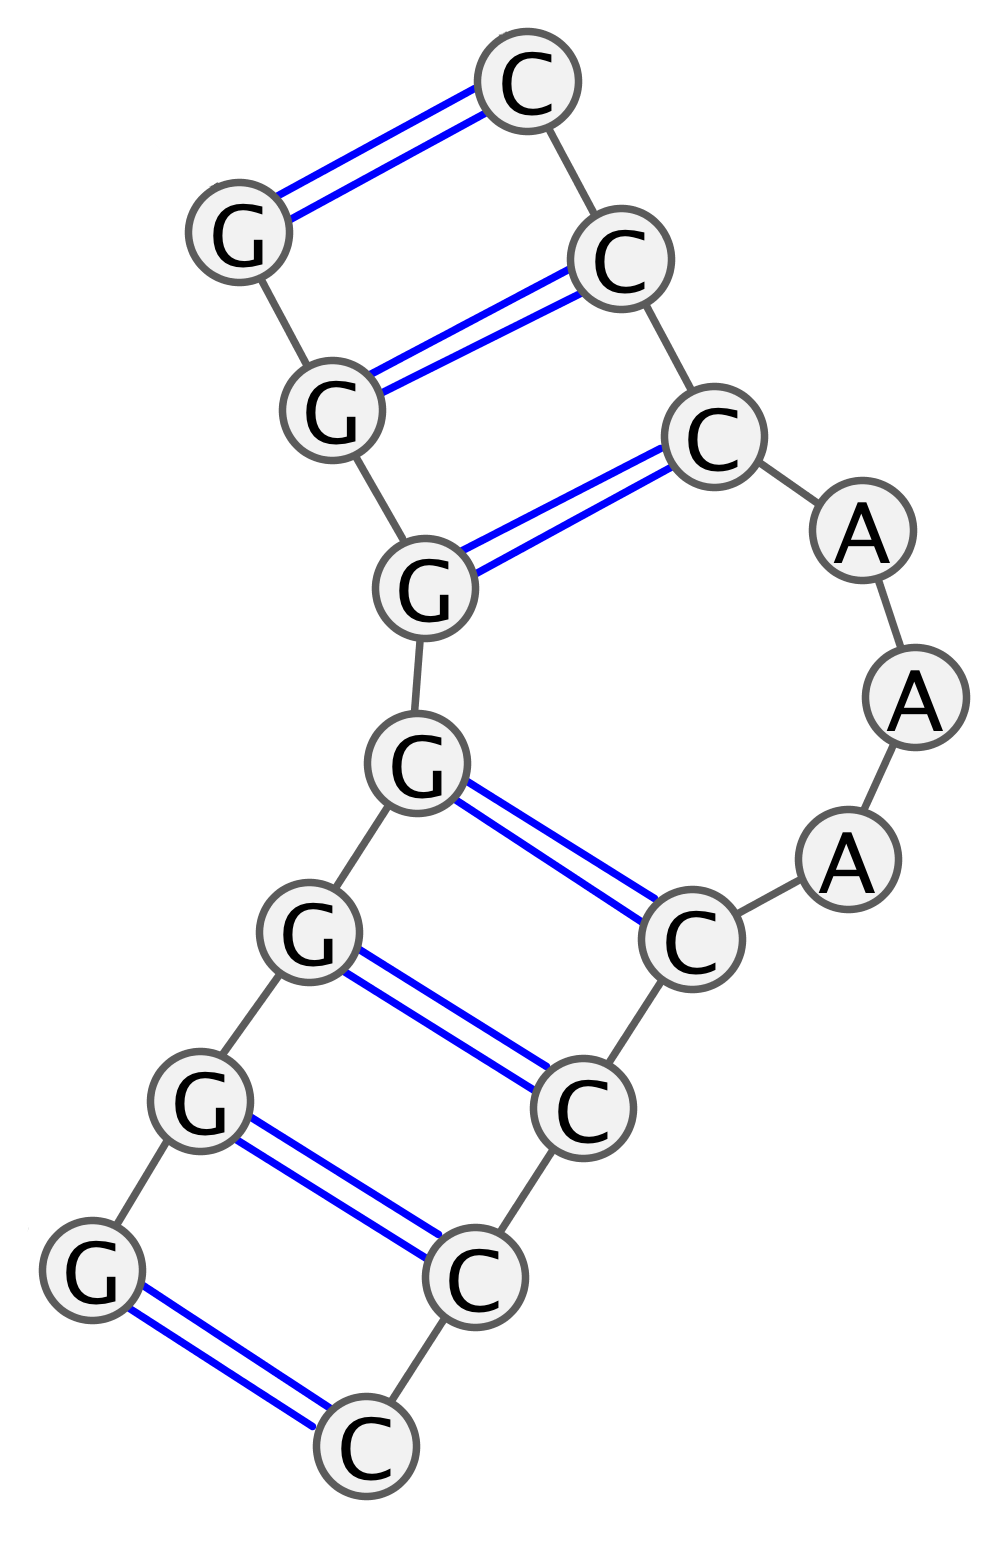
\includegraphics[width=4.5cm]{./pictures/bulge_varna.PNG} Internal loop\linebreak  (code: 0--3) \tabularnewline
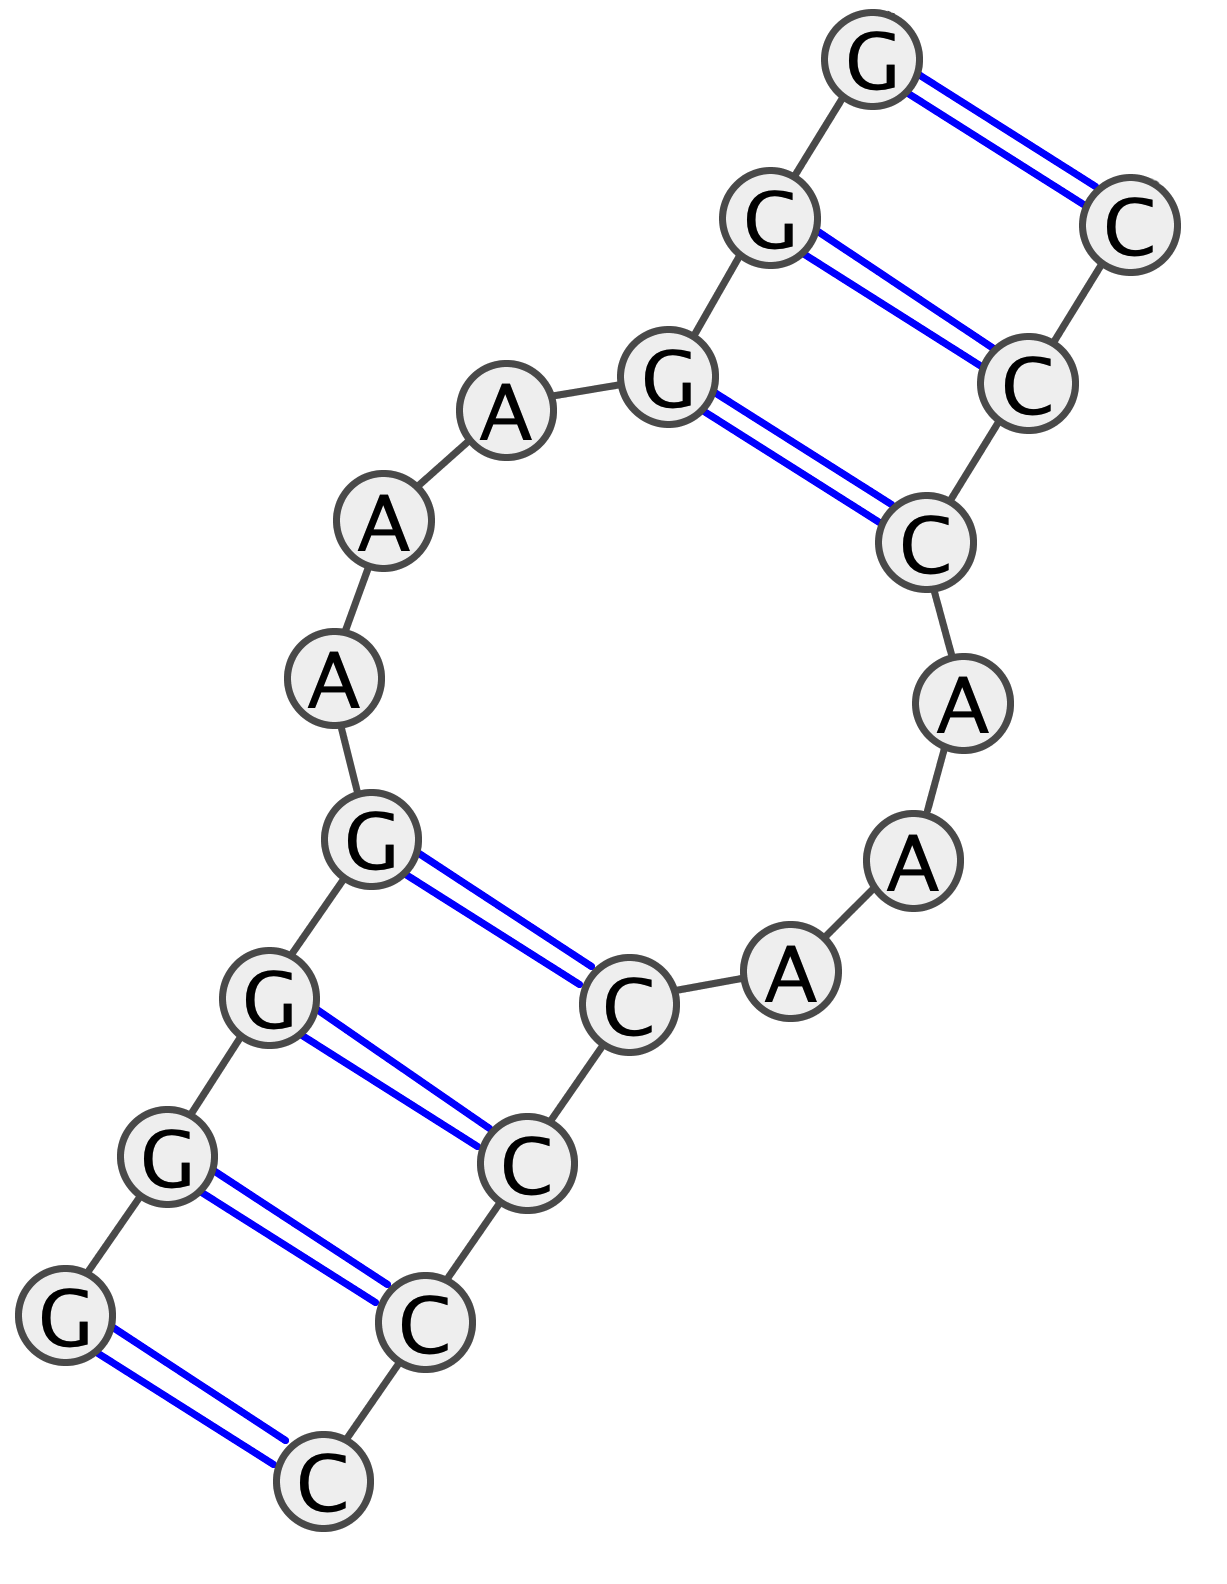
\includegraphics[width=5cm]{./pictures/interior_varna.PNG} Internal loop \linebreak  (code: 3--3) & 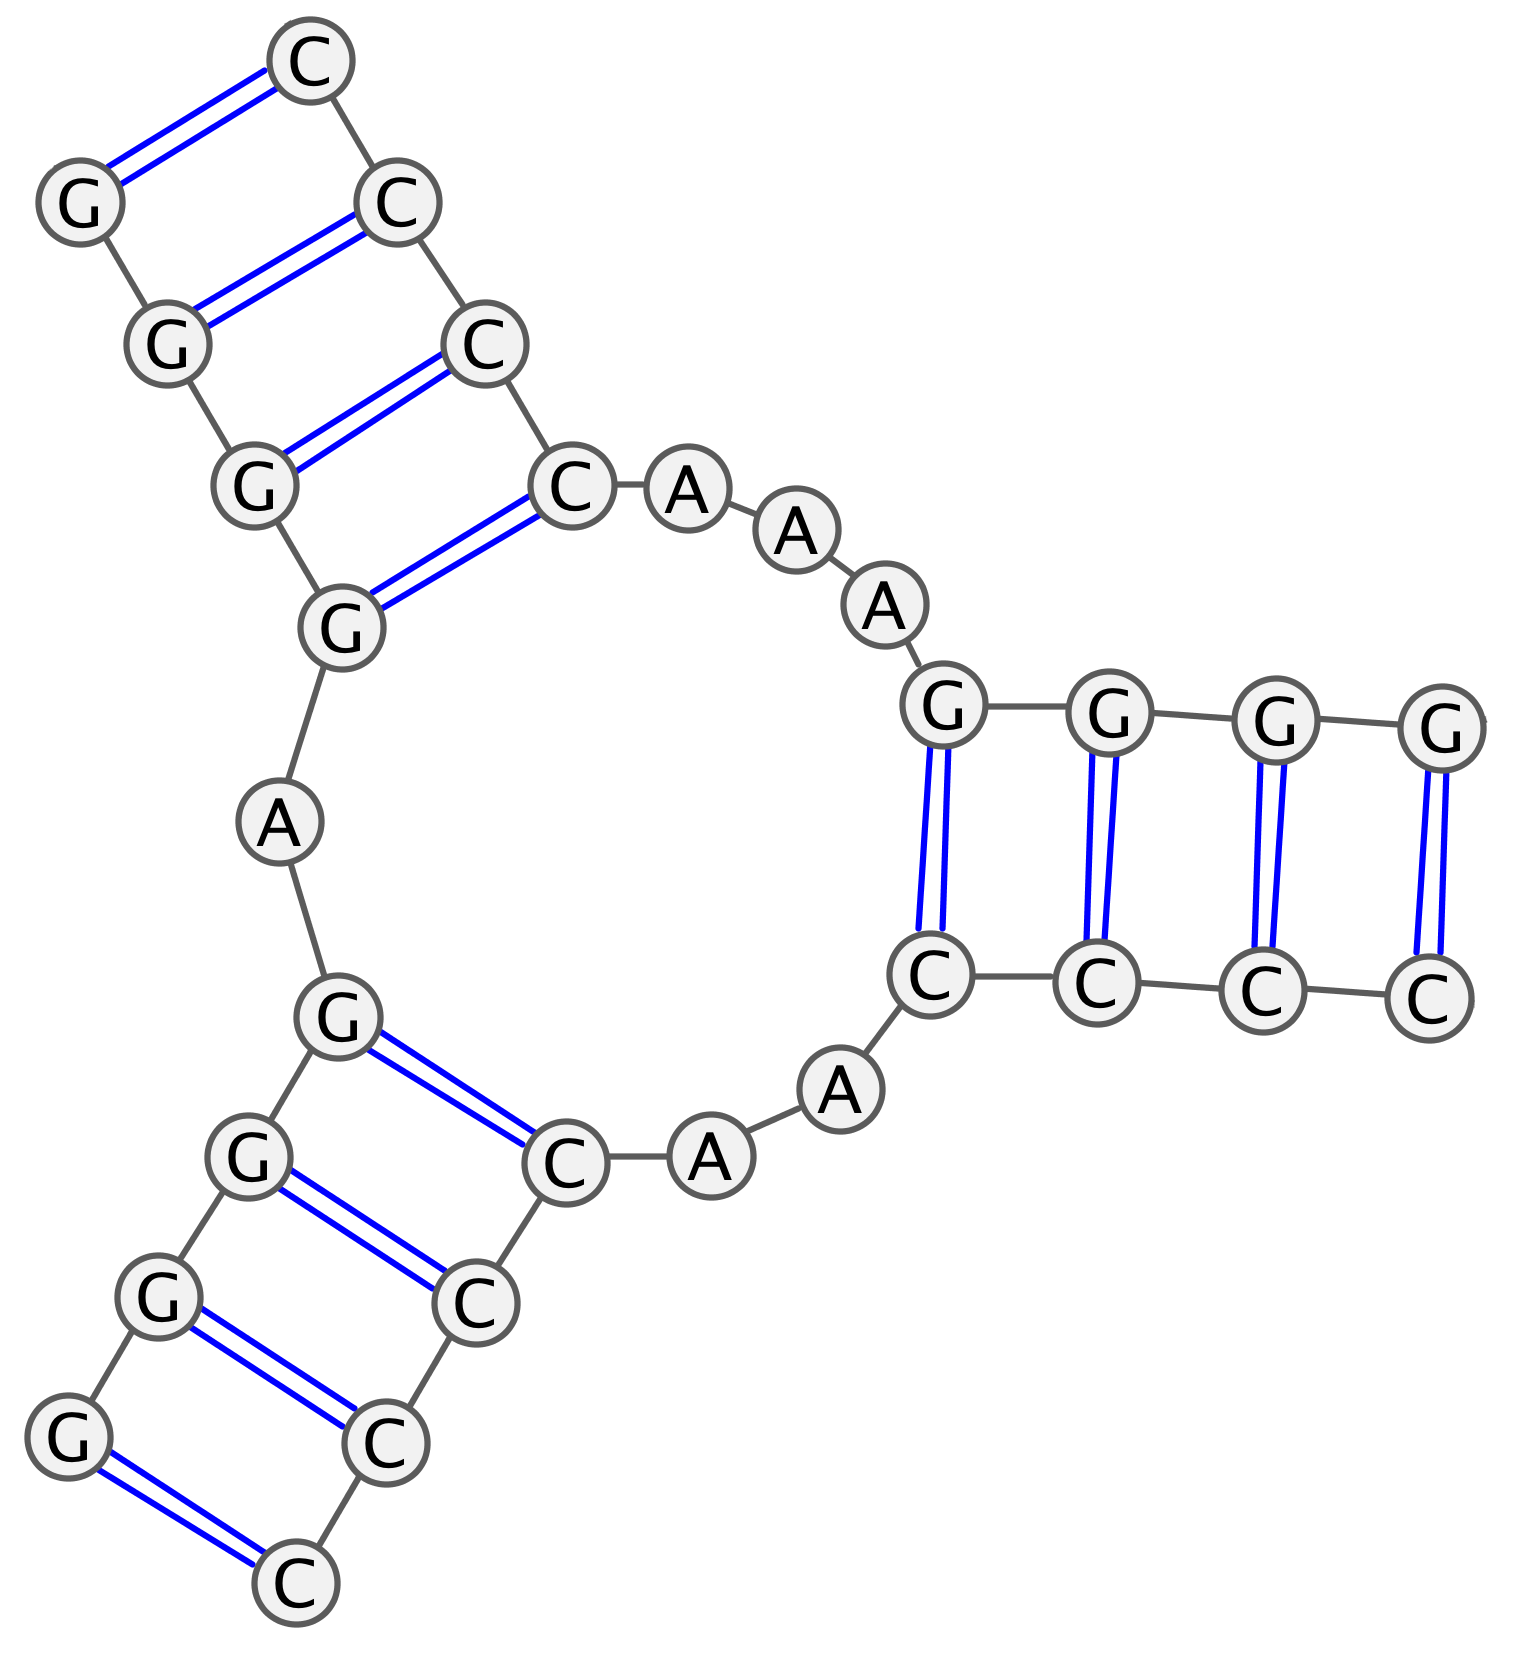
\includegraphics[width=5.5cm]{./pictures/multibranched_varna.PNG} Multi-branched loop\linebreak (code: 2--3--1) & 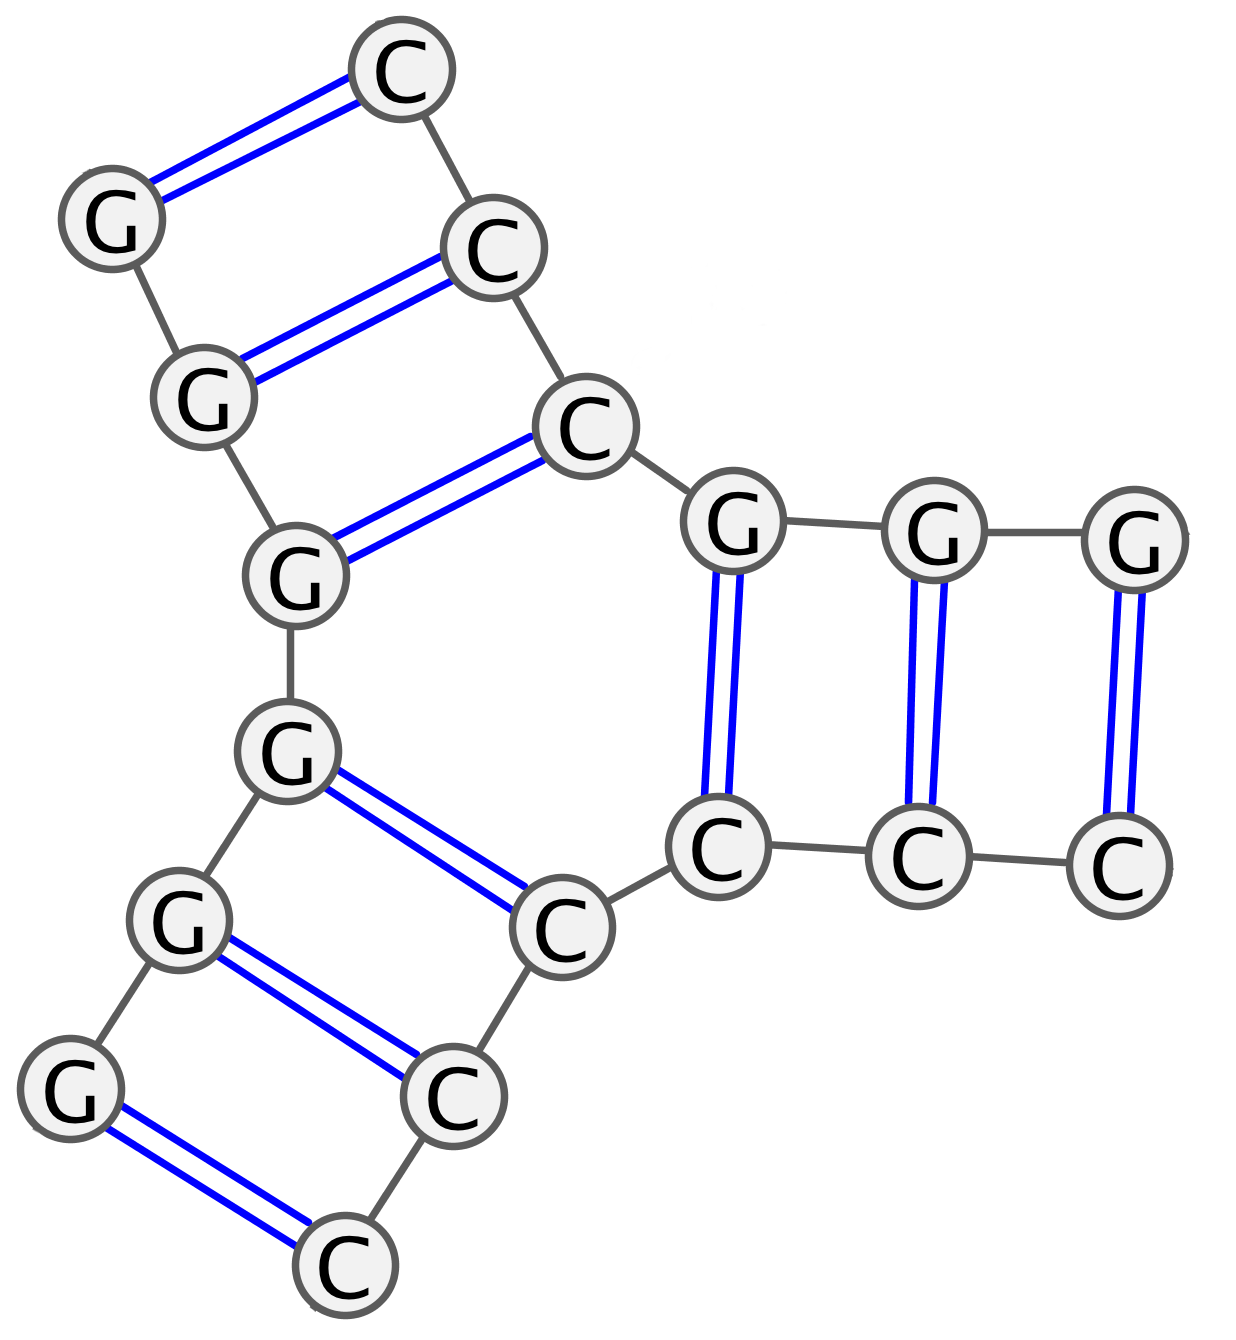
\includegraphics[width=5cm]{./pictures/junction_varna.PNG} 3-way junction\linebreak (code: 0--0--0)  \tabularnewline
&& \tabularnewline
\end{tabular}
\end{table}

\newpage

\paragraph{The RNA motif} \label{RNA_motifs} nomenclature (i.e., a loop, bulge or junction) can be inaccurate and misleading. The program uses the numerical description of motifs that should be easily understandable. The numbers correspond to the numbers of unpaired nucleotides between the paired nucleotides. Therefore, a four nucleotide loop at the end of a hairpin is represented by a single number 4. A symmetric bulge loop, with both bulges of the length of three is represented by two numbers: 3--3 and a three-way junction, without unpaired nucleotides is represented by three zeros: 0--0--0.  Examples of RNA secondary structure motifs with their labels are presented in Table \ref{RNAsecondaryStructures}. 

\subsubsection{Motif-search algorithm}
The motif-search algorithm uses a list-representation of the RNA-secondary structure that contains the list of all WC pairs. As shown in Figure \ref{MotifsAlgorithm} the algorithm detecting helices and other secondary structure motifs walks through the list and stores the information about the visited nucleotides. 

As long as there are paired nucleotides, the algorithm stores the information about the helix (steps 1 and 15 in Figure \ref{MotifsAlgorithm}). When it encounters the end of the helix (steps 2 and 16) -- i.e., an unpaired nucleotide ahead of a pair, it starts to travel (search) around the motif. It stores the first pair (as the beginning pair) and goes to the index stored in the list. Then for as long as it encounters an unpaired nucleotide it moves back -- with decreasing indexes (steps 3 to 13 and steps 16 to 22). When another pair is encountered, the algorithm goes into the indicated position and again moves back (steps 10 and 16). This motif-search ends when the algorithm finds itself one step ahead of the starting index (steps 13, 22). The number of "jumps" represents the number of unpaired nucleotides in between. After one motif is found and classified, the algorithm jumps one step further to the last seen pair (steps 14 and 23). The algorithm stops searching for the motifs and helices when the index is larger than the value stored in the list (step 23). 

\begin{figure}[h!]
\centering
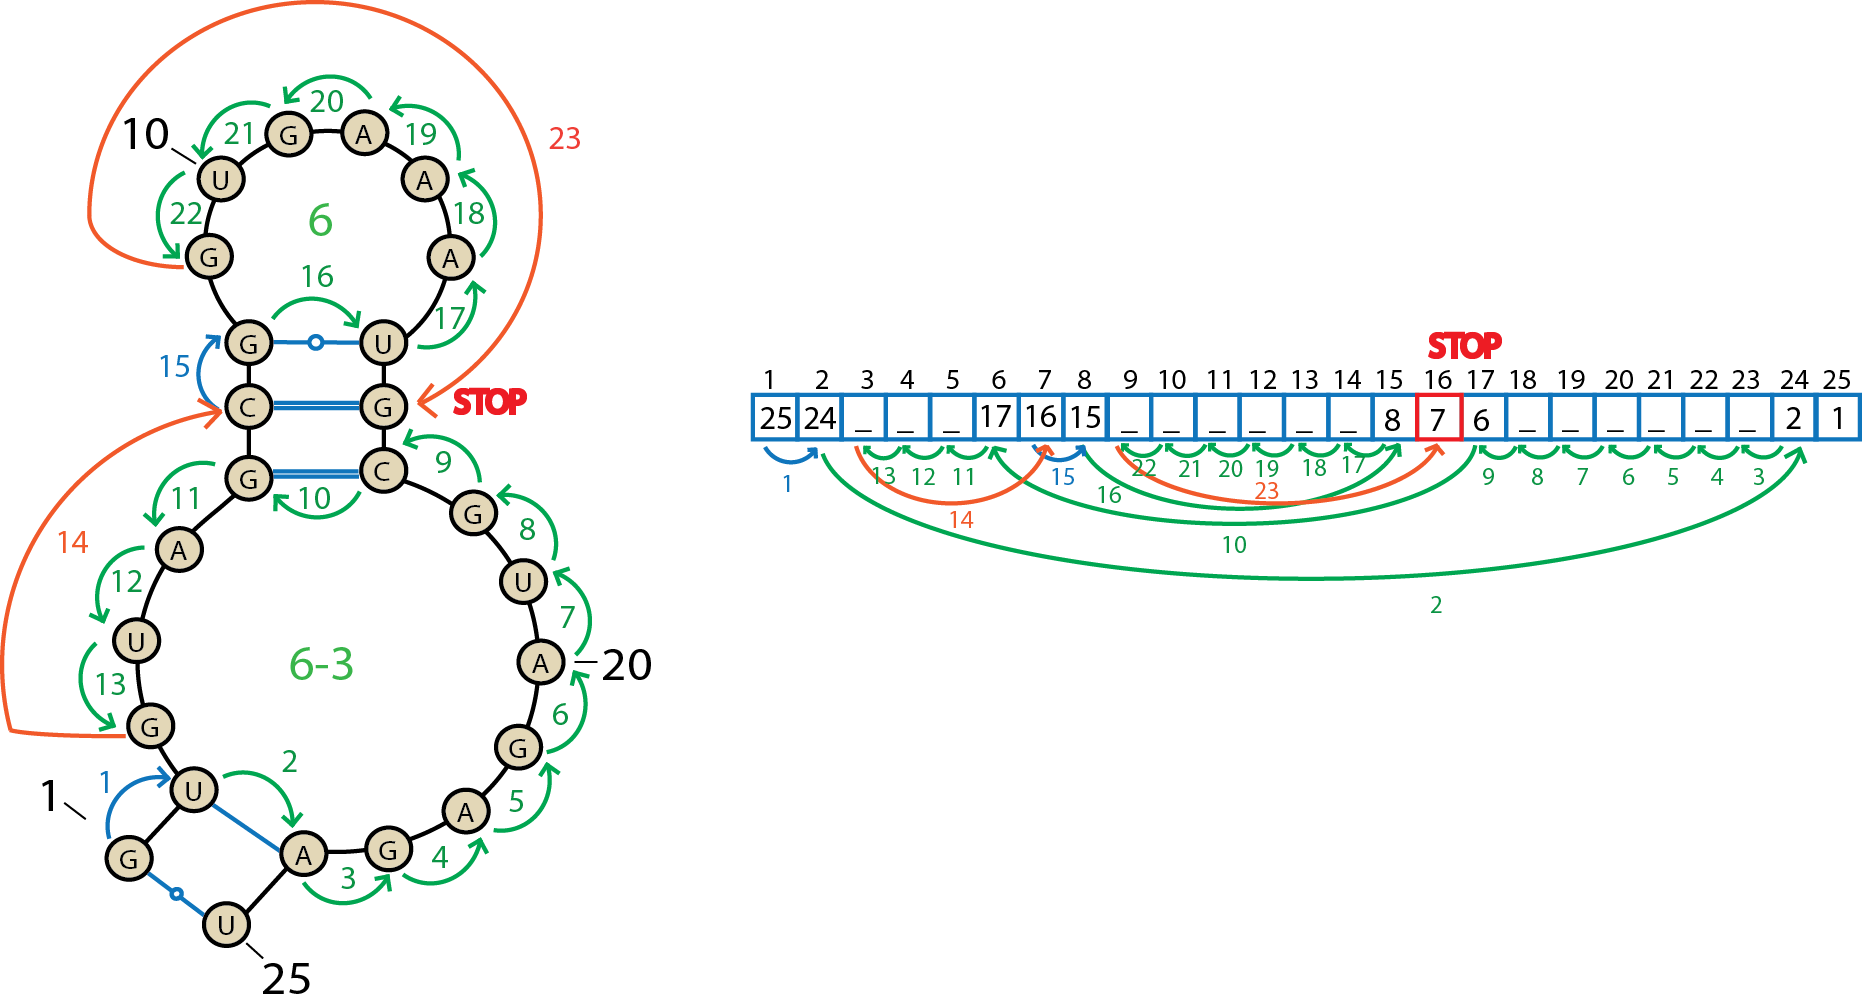
\includegraphics[width =\textwidth]{./pictures/algorithm.png}
\caption{A scheme presenting the steps of the algorithm that finds and classifies the motifs in the RNA structures. The numbers correspond to the step number. Green arrows correspond to the structural motif and blue to  helices. The orange lines denote the jumps after finishing the motif. The STOP sign indicates the position where the algorithm stops.}
\label{MotifsAlgorithm}
\end{figure}

As a result of a single frame analysis, the algorithm returns a list of all pairs, motifs and numerical characterization of all nucleotides. Every nucleotide is characterized with the number of hydrogen bonds it created and the description of its partners:

\begin{verbatim}
G538 , 538 , 3-C513A539:1 , 2-C513:2 , 3-C513:7
\end{verbatim}

where first comes the type of the nucleotide with its PDB code, second only the PDB code, followed by the lists of pairs this nucleotide created during the trajectory or in the uploaded conformation set. The number of hydrogen bonds is preceding the hyphen. Next, there can be more than one nucleotide listed -- what indicates a triplex. The number after a semicolon is the number of frames in which this pair or triplex were detected.

\newpage
\section{Analysis of trajectories or many RNA/DNA conformations}
If multiple RNA/DNA conformations (e.g. from molecular dynamics trajectory) have to be analyzed and classified, every frame/conformation is characterized as previously described. The main output of the program is a set of {\tt .csv} files listing all the pairs and motifs: helices, triplexes, pseudoknots etc., their occurrence and frame numbers in which the considered structure was present, its topology and participating nucleotides. Description of the output files can be found in Section~\ref{OutputFiles}.

\subsection{Clustering}\label{Clustering}
To recognize and characterize the changes in the secondary structure of the RNA/DNA molecule that may occur in the trajectory, we have to cluster the detected secondary structure motifs. Clustering is parameterized with two user-defined parameters: \\
\begin{itemize}
\item {\tt time\_cutoff} that defines the minimal percentage of frames in which the motif has to be present in order to be classified.
\item {\tt margin} that defines the minimal percentage of similarities between the two motifs to belong to the common cluster. 
\end{itemize}

The first step is to filter the motifs i.e., remove the rare motifs  and leave only the significant ones. Filtering of motifs is done according to the number of frames the motif appeared in. Below we show an exemplary list of motifs after removing rare motifs:

\begin{figure}[h!]
\centering
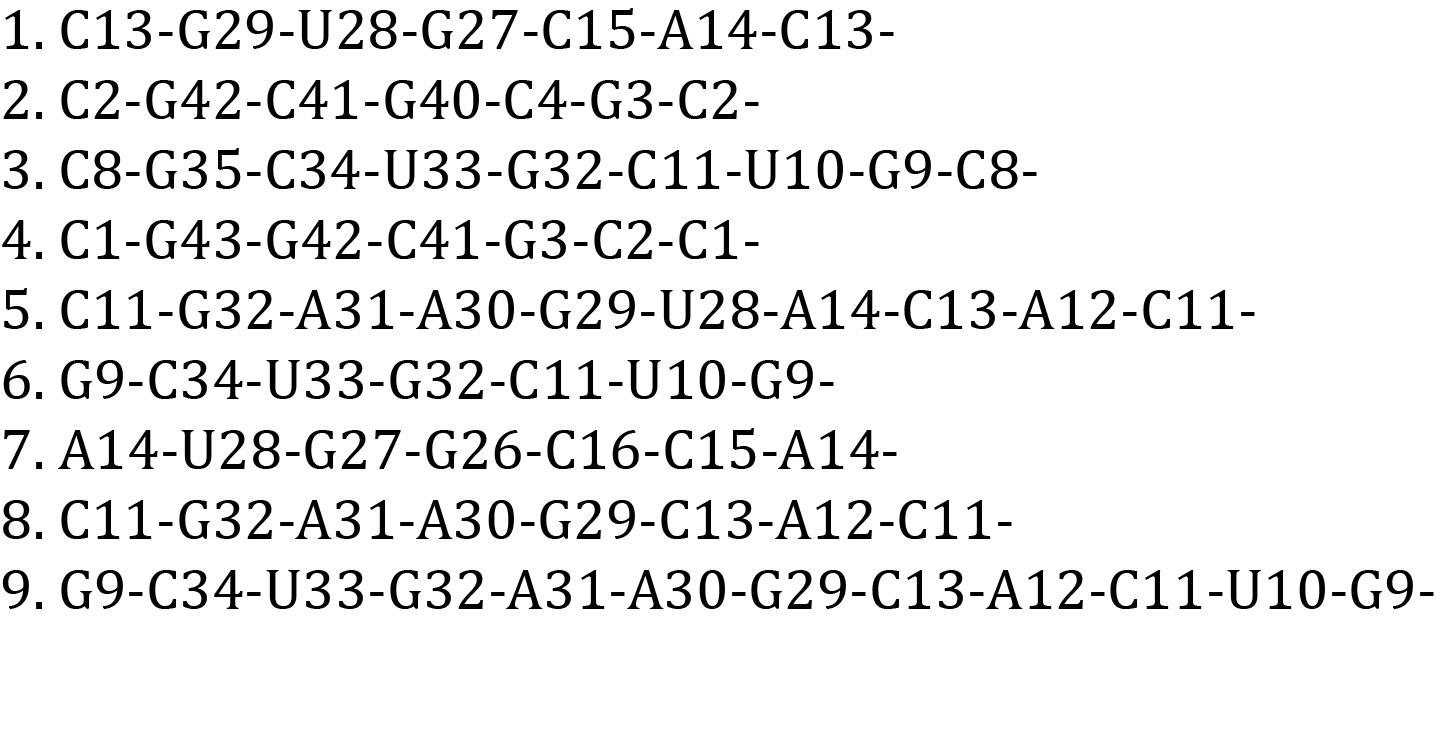
\includegraphics[scale=1]{./pictures/cluster_motif_step1.png}
\caption{First step of clustering.}
\label{MotifsClusteringStep1}
\end{figure}

Second, the motifs' distance matrix is computed. The distance between the motifs is the number of their common nucleotides. The order of the nucleotides is not taken into account:
\begin{figure}[h!]
\centering
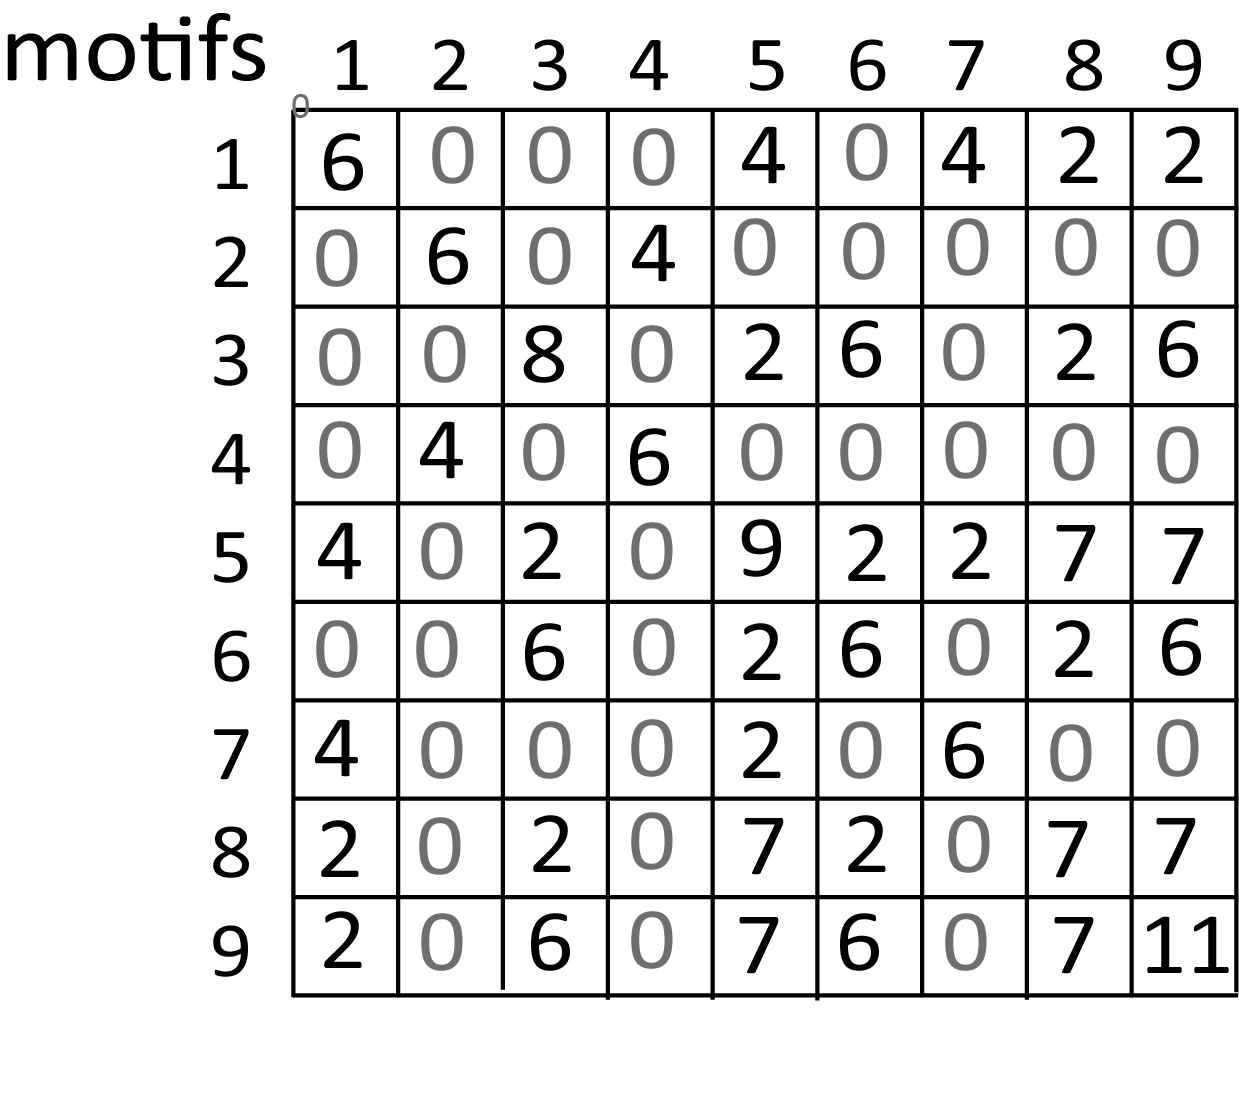
\includegraphics[scale=0.6]{./pictures/cluster_motif_step2.png}
\caption{Exemplary motif distance matrix}
\label{MotifsClusteringStep2}
\end{figure}

\newpage
Third, the partners for all motifs are denoted. The partner has to satisfy the distance requirement expressed by the equation shown below:
\begin{figure}[h!]
\centering
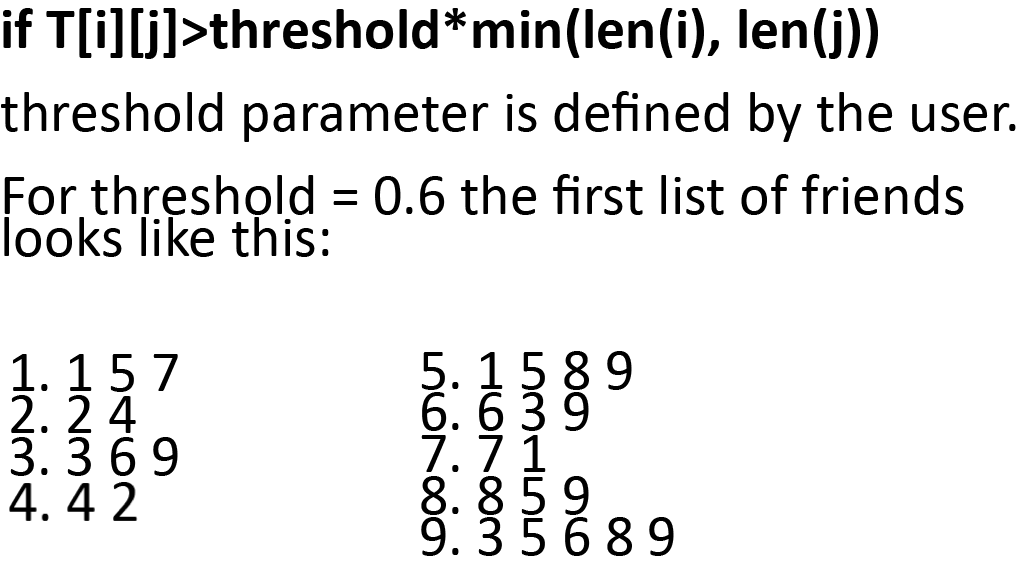
\includegraphics[scale=1]{./pictures/cluster_motif_step3.png}
\label{MotifsClusteringStep3}
\caption{Equation with the distance requirement that motifs have to satisfy to be partners}
\end{figure}

Next, the motif with the longest list of partners is incorporated as the first one to the first cluster (numbered zero). The motifs already assigned to the first cluster have to be crossed out from the rest. Then the second longest motif is chosen, the picked motif is crossed out, and so on.  

\begin{figure}[h!]
\centering
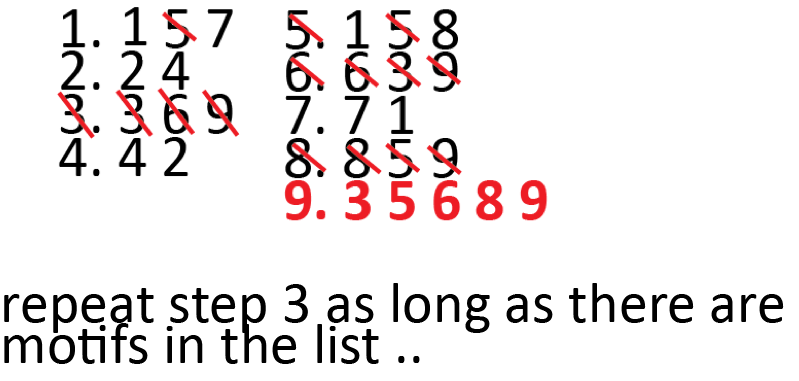
\includegraphics[scale=1]{./pictures/cluster_motif_step4.png}
\label{MotifsClusteringStep4}
\caption{Removal of partners from the list of motifs}
\end{figure}

\begin{figure}[h!]
\centering
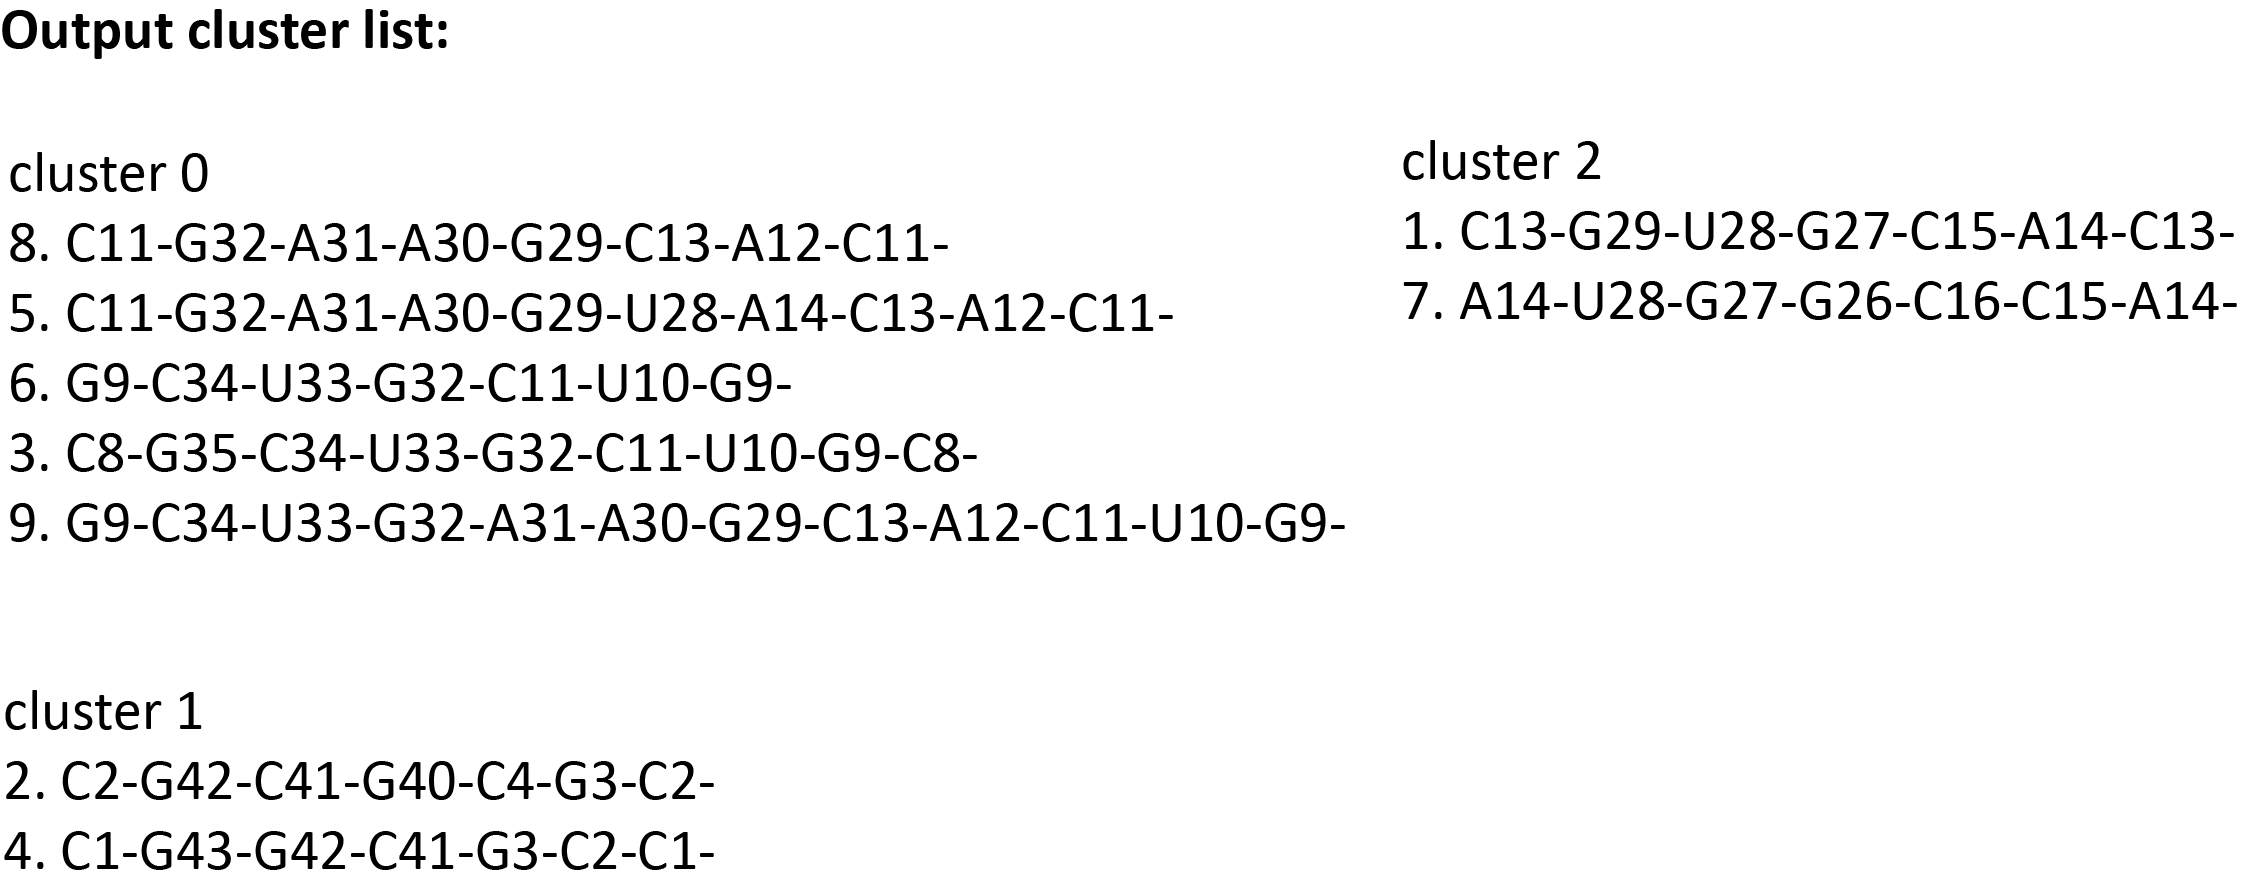
\includegraphics[scale=1]{./pictures/cluster_motif_step5.png}
\label{MotifsClusteringStep5}
\caption{Result of the clusterization process.}
\end{figure}

Additionally, the average clusters are returned. The list consists of the longest motif for every cluster and the two vectors of float values describing every nucleotide participating in the representative motif. The float vectors represent the average number of hydrogen bonds created by a nucleotide in both WC-WC pairs and other interactions. We hope to show the average secondary structure of the molecule within the tertiary structure description. While analyzing the whole output generated by the script, one can understand the complex description of the RNA structure in the dynamics.

\newpage
\section{Visualization}\label{Visualization}
MINT enables many different ways of data visualization. The user can display a colored input PDB structure according to several parameters (motifs, secondary and tertiary contacts, electrostatic energies, VDW energies) both in the {\tt Single} and {\tt Trajectory} mode. 

For visualization we suggest to install the following programs:
\begin{itemize}
\item {\tt VMD}\cite{Humphrey1996}, or {\tt Chimera}~\cite{Pettersen2004} for tertiary structure visualization.
\item {\tt RNAMovies} for secondary structure visualization changes in the trajectory\\(\url{http://bibiserv.techfak.uni-bielefeld.de/rnamovies/}).
\end{itemize}

\subsection{Representing motifs on the tertiary structure} 
\label{VMD}
This feature (available only in the {\tt Mode: Single}) works through creating representations of the regions of the nucleic acid molecule in the input PDB file using the {\tt VMD} program \cite{Humphrey1996}. In {\tt VMD} one can represent fragments of a molecule using different representations and colors, all can be managed from {\tt Graphical Representations} menu ({\tt Graphics > Representations}). The {\tt \_vmd\_run.tcl} script loads the structure and creates {\tt Reps} for every motif and helix in the structure what results with a view of the three-dimensional molecule colored accordingly to the detected structural components:

\begin{itemize}
\item helices: yellow ({\tt VMD} color code:4)
\item pseudoknots: tan ({\tt VMD} color code:5)
\item triplexes: silver ({\tt VMD} color code:6)
\item loops: green ({\tt VMD} color code:7)
\end{itemize}

If the {\tt VMD} program is in your PATH you can turn on the {\tt vmd} parameter and it will launch automatically. Otherwise, you can do it manually by going into your {\tt MINT} inputs/outputs directory and typing in the terminal:

{\tt your\_vmd\_location$\backslash$vmd -e \_vmd\_run.tcl }

\begin{figure}[h!]
\centering
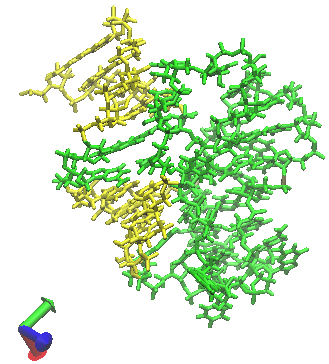
\includegraphics[scale=0.8]{./pictures/motifs_vmd.png}
\caption{The result of running the exemplary structure {\tt \_vmd\_run.tcl } script in the {\tt VMD} program after changing the display into {\tt Orthographic} and the background color to white.}
\end{figure}

\subsection{Representing hydrogen bonding and stacking on the tertiary structure} 
The {\tt MINT} program outputs several PDB files each with the B-factor column  replaced for each nucleotide atom line with:
\begin{itemize}
\item {\tt \_Hbonds-WC.pdb} -- the number of hydrogen bonds in the WC pairs created by a given nucleotide,
\item {\tt \_Hbonds-non-WC.pdb} -- the number of hydrogen bonds in the non-WC pairs created by a given nucleotide,
\item {\tt \_Hbonds-total.pdb} -- the number of hydrogen bonds in both  WC and non-WC pairs created by a given nucleotide,
\item {\tt \_Stacking-Coulomb.pdb} -- the Coulomb energy for a given nucleotide  (the sum of all electrostatic interactions the nucleotide is involved in),
\item {\tt \_Stacking-VDW.pdb} -- the Van der Waals energy for a given nucleotide (the sum of all interactions the nucleotide is involved in),
\item {\tt \_Stacking-total.pdb} -- the sum of the Van der Waals and Coulomb energies. 
\end{itemize}

For a trajectory these PDB files contain the average values (over all frames). Here, we  describe how to visualize the data outputted by {\tt MINT} using the {\tt VMD} or {\tt Chimera}.

\paragraph{VMD}
{\tt VMD} is a powerful tool with a complete user guide and tutorial that can be found at (\url{http://www.ks.uiuc.edu/Research/vmd/}).
First, the user has to open the {\tt VMD} program and load one of the PDB files, by choosing the {\tt New Molecule} from the {\tt File} drop-down menu as shown below:

\begin{figure}[h!]
\centering
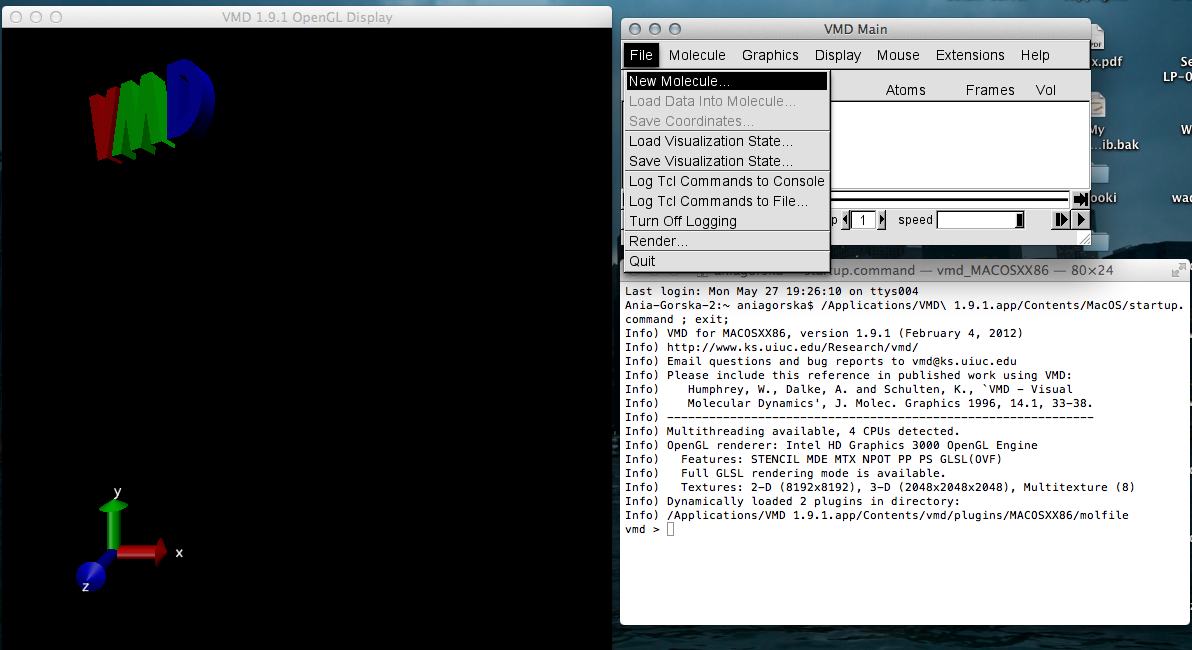
\includegraphics[scale=0.4]{./pictures/vmd1.png}
\caption{Loading a PDB file into the {\tt VMD} program}
\end{figure}

Second, one has to {\tt Browse} and {\tt Load} a PDB file of choice:
\begin{figure}[h!]
\centering
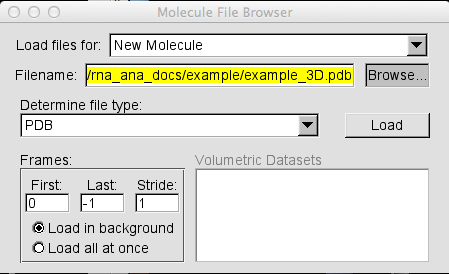
\includegraphics[scale=0.4]{./pictures/vmd2.png}
\caption{Loading a PDB file into {\tt VMD} program}
\end{figure}
\newpage
Having uploaded the structure, one needs to open the {\tt Representations} window from the {\tt Graphics} drop-down menu:
\begin{figure}[h!]
\centering
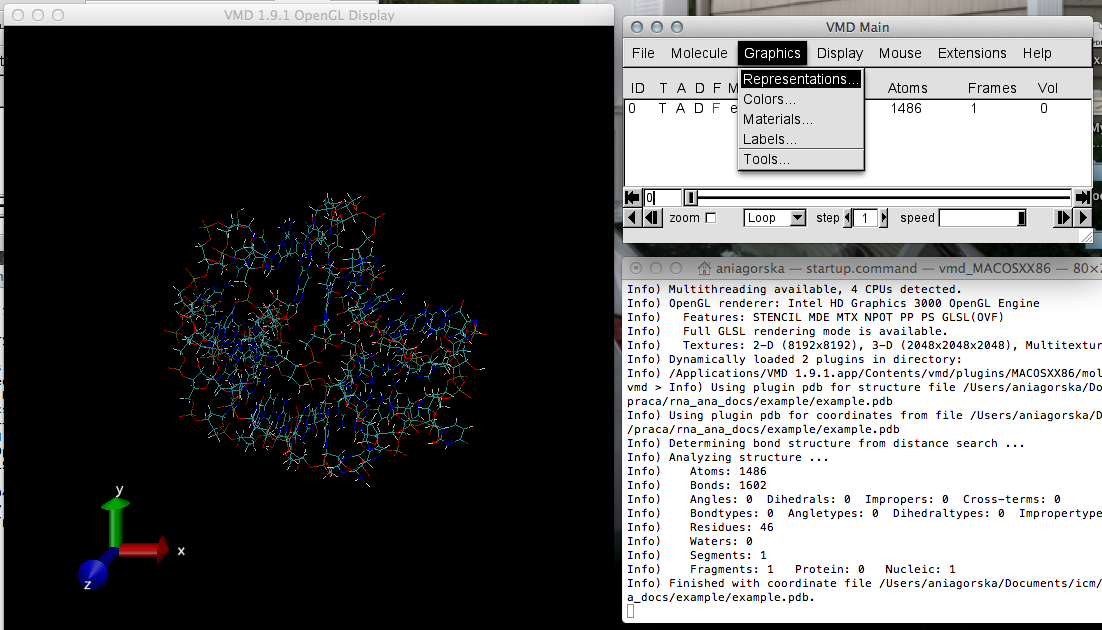
\includegraphics[scale=0.4]{./pictures/vmd3.png}
\caption{Opening the representation window in {\tt VMD}}
\end{figure}

The {\tt Representations} menu allows one to create various representations. To color the structure by the B-factor column in the PDB file, we suggest to change the {\tt Drawing Methods} into the {\tt New Cartoon} and the {\tt Coloring Method} into the {\tt Beta}:

\begin{figure} [h!]
\begin{center}
\subfigure[]{
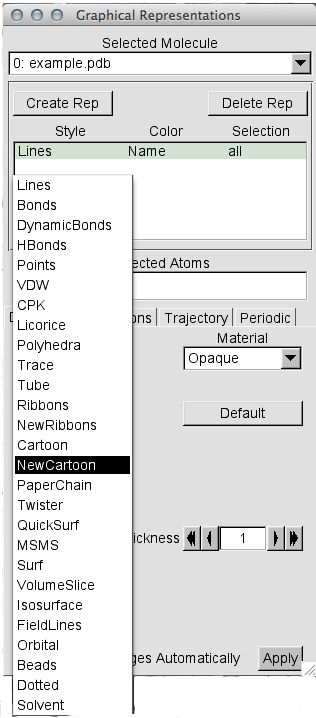
\includegraphics[scale=0.325]{pictures/vmd4.png}}
\subfigure[]{
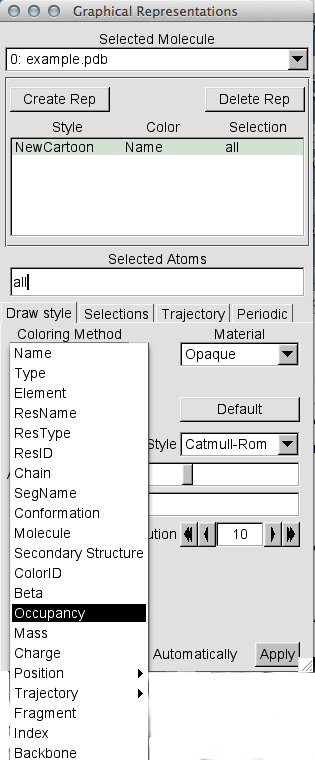
\includegraphics[scale=0.3]{pictures/vmd5.png}}
\end{center}
\caption{Choosing {\tt Drawing} and {\tt Color Methods} in the VMD program}
\end{figure} 

\newpage
Next, the color scale can be altered through {\tt Graphics} $>$ {\tt Color} $>$ {\tt Color Scale}:

\begin{figure}[h!]
\centering
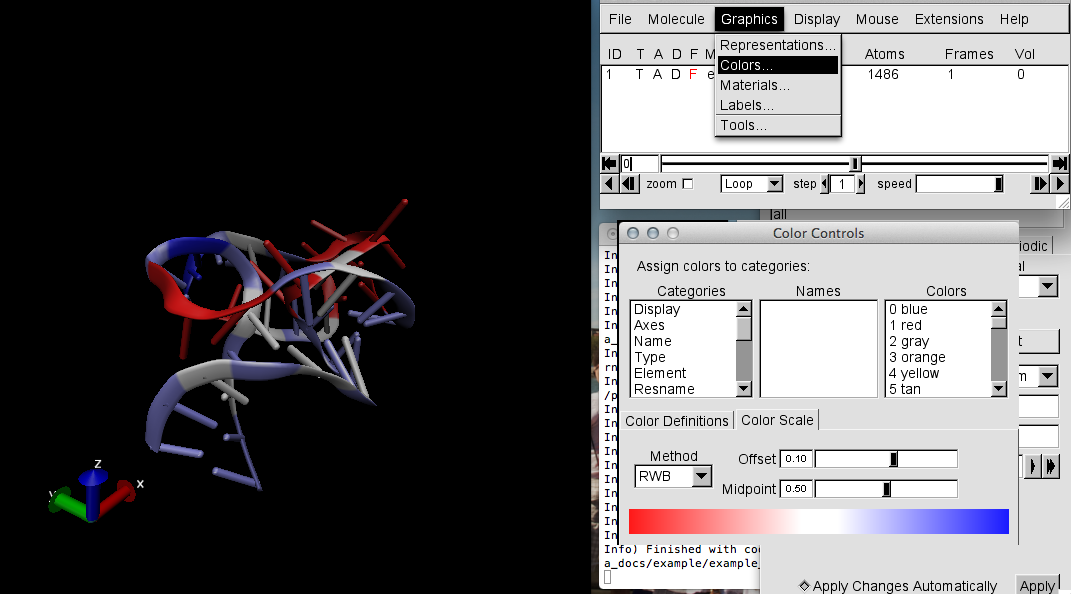
\includegraphics[scale=0.4]{./pictures/vmd6.png}
\caption{Changing the color scale}
\end{figure}

If you proceed in the same way with more than one PDB structure you can use the {\tt Move} tool ({\tt Mouse} $>$ {\tt Move} $>$ {\tt Molecule}) and view the colored structures at the same time as it is shown in Figure \ref{3Ddifferent}.

\begin{figure}[h!]
\begin{center}
\subfigure[{\scriptsize Number of hydrogen bonds in WC pairs}]{
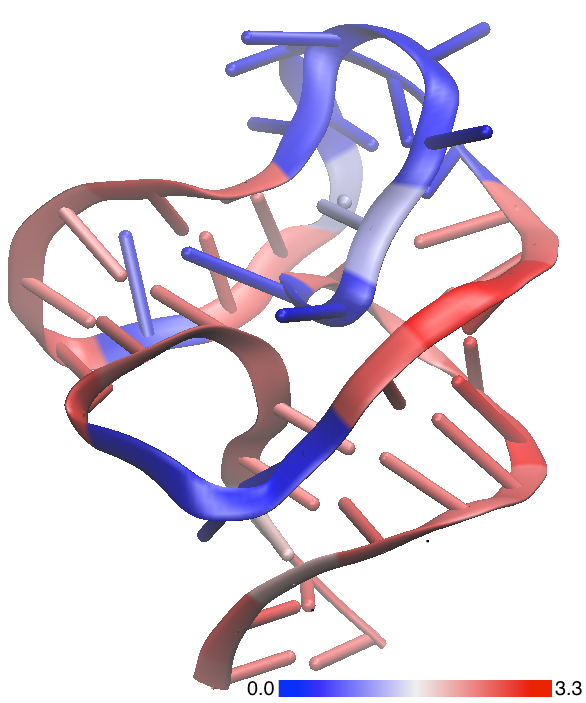
\includegraphics[scale=0.15]{./pictures/example_2D_3d.png}}
\subfigure[{\scriptsize Number of hydrogen bonds in non-WC pairs}]{
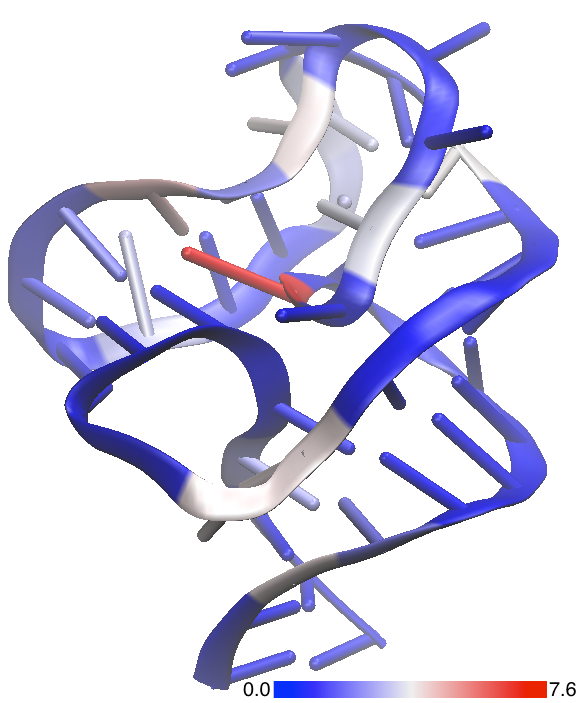
\includegraphics[scale=0.15]{pictures/example_3D_3d.png}}
\subfigure[{\scriptsize VDW energy per nucleotide}]{
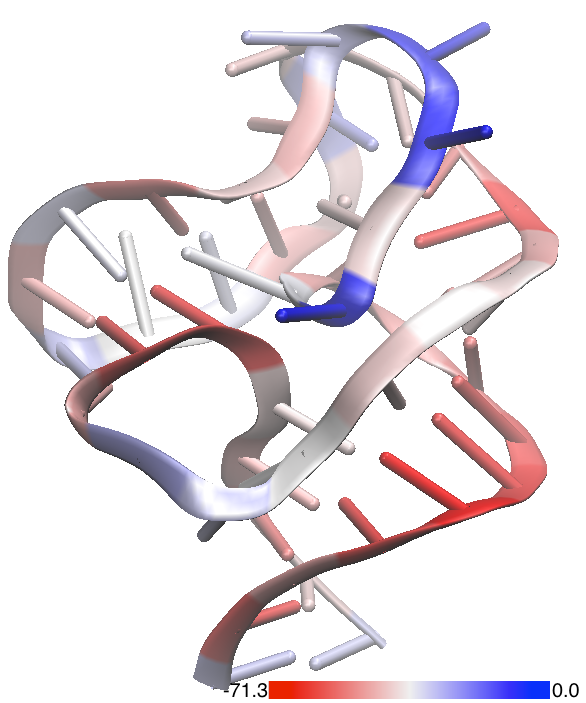
\includegraphics[scale=0.15]{pictures/example_vdw_3d.png}}
\subfigure[{\scriptsize Coulomb energy per nucleotide}]{
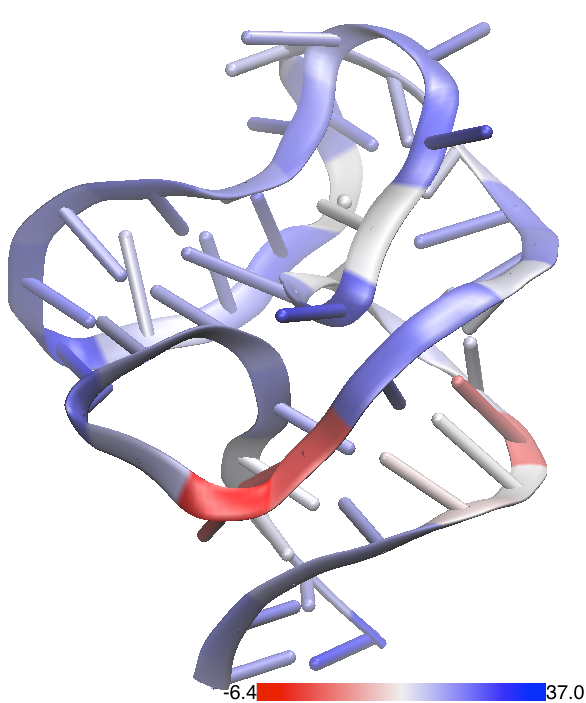
\includegraphics[scale=0.15]{pictures/example_coulomb_3d.png}}
\subfigure[{\scriptsize Sum of stacking energy per nucleotide}]{
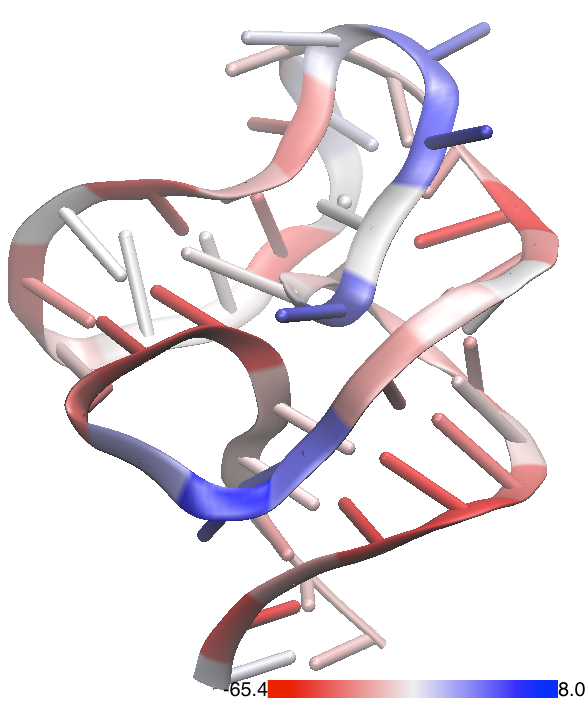
\includegraphics[scale=0.15]{pictures/example_stacking_3d.png}}
\end{center}
\caption{The starting tertiary structure rRNA fragment (nucleotides 500 to 545) colored according to various computed descriptors averaged from the trajectory (the same exemplary fragment was shown before in Figure \ref{varna}). Figures created with the use of the {\tt VMD} program and the {\tt MINT} output PDB files. All energy is expressed in kcal/mol.}
\label{3Ddifferent}
\end{figure} 



\paragraph{Chimera}
High-quality 3D visualizations can be also prepared with the {\tt Chimera} software (details on how to use the program can be found at (\url{https://www.cgl.ucsf.edu/chimera/}). The user has to open {\tt Chimera} and load one of the PDB files and next, choose from the {\tt Tools} menu the {\tt Depiction} section and click on the {\tt Render by Attribute} as shown in Figure~\ref{chimera1}.

\begin{figure}[h!]
\centering
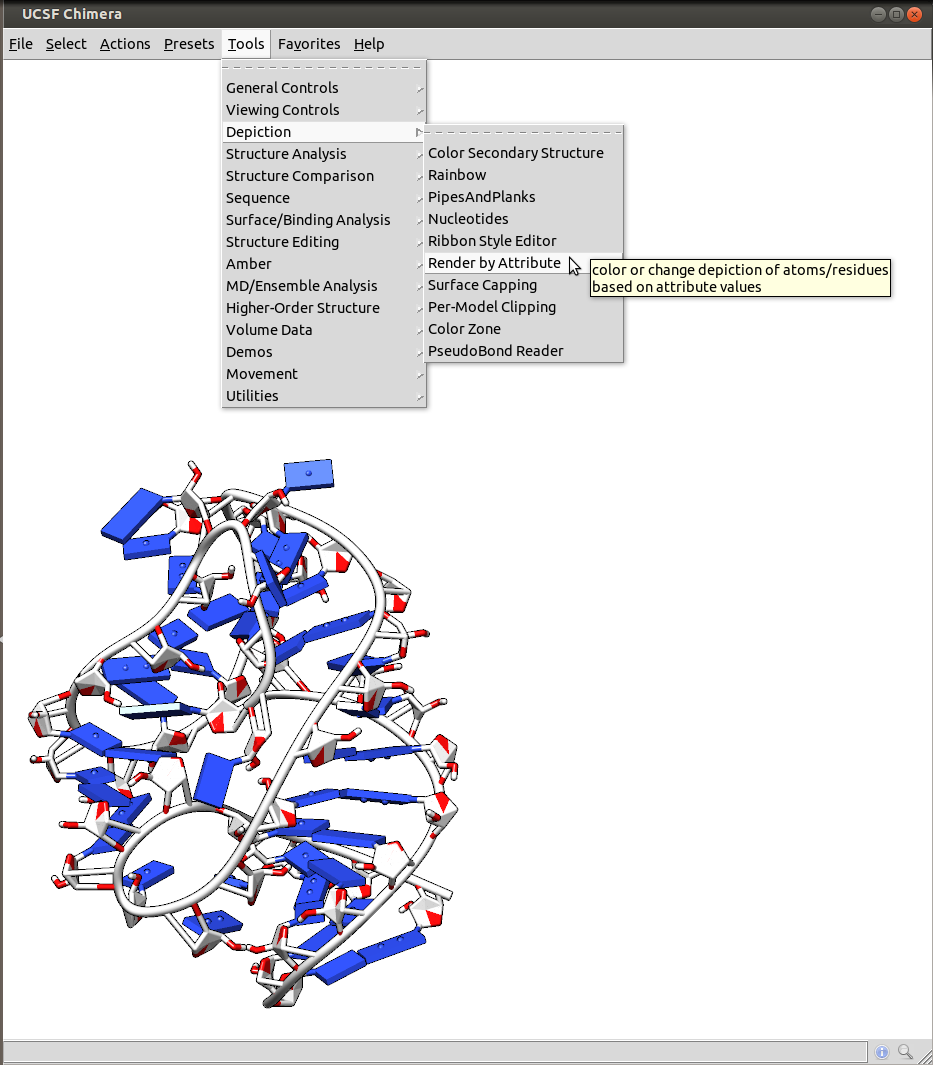
\includegraphics[scale=0.27]{./pictures/chimera1.png}
\caption{Render by attribute menu in Chimera}
\label{chimera1}
\end{figure}

\newpage
In the opened window (Figure~\ref{chimera22}) the user chooses attributes of {\tt residues} instead of default {\tt atoms}. The {\tt Attribute:} should be changed to {\tt average -> bfactor}. Then the color scale and palette can be chosen and the color key can be created. Two exemplary pictures rendered in {\tt Chimera} are presented in Figure~\ref{chimera-pictures}.
\begin{figure}[!h]
\centering
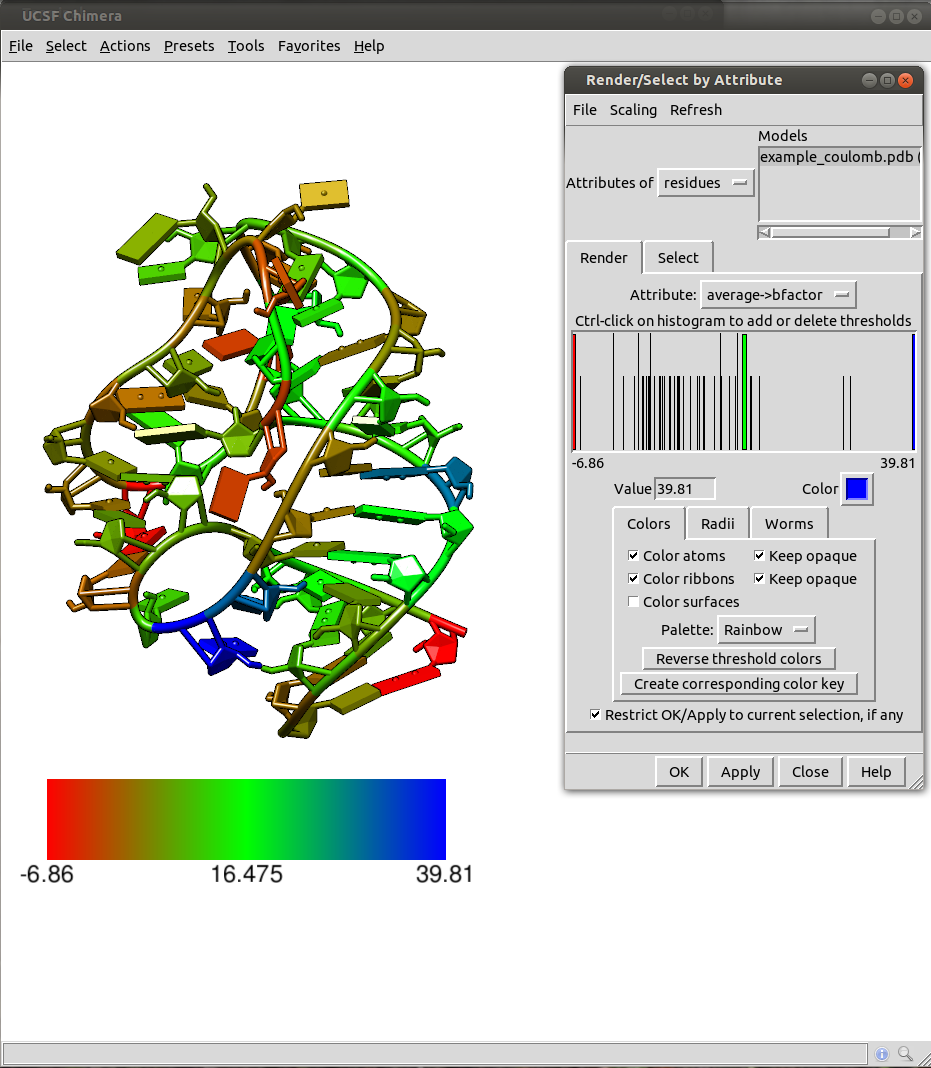
\includegraphics[scale=0.22]{./pictures/chimera2.png}
\caption{Rendering the structure by attribute in the {\tt Chimera} program using the PDB file created by {\tt MINT}}
\label{chimera22}
\end{figure}


\begin{figure}[!h]
\hspace*{\fill}%
\subfigure[Average number of WC hydrogen bonds per nucleotide]{
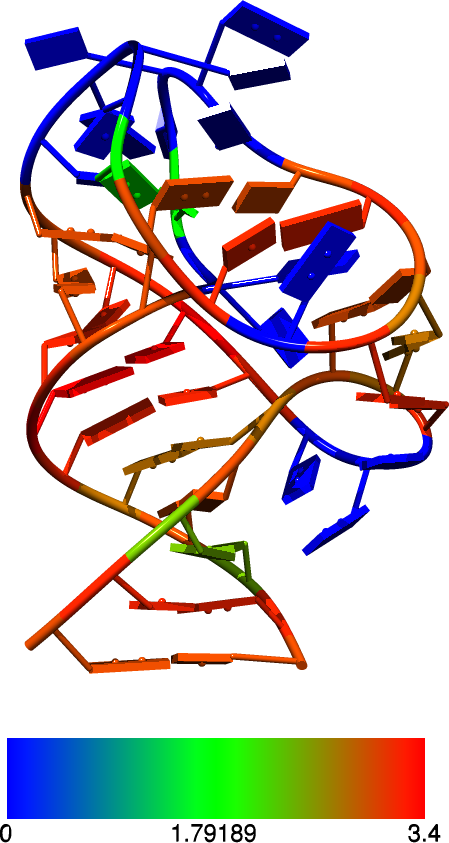
\includegraphics[scale=0.22]{./pictures/chimera-2D.png}}\hfill%
\subfigure[Average energy (in kcal/mol) of stacking interaction per nucleotide]{
\includegraphics[scale=0.22]{./pictures/chimera-stacking.png}}
\hspace*{\fill}%
\caption{Exemplary pictures created with the use of the Chimera program and the PDB files created by MINT}
\label{chimera-pictures}
\end{figure}

\newpage
\subsection{Representing secondary structure changes} 
Analysed trajectory can be visualized in the secondary structure representation with the RNAMovies \cite{Evers1999} program. {\tt MINT} returns the {\tt RNAStructML.xml} file containing the trajectory of the secondary structure. For every frame the dot-bracket representation is written into the .xml file. This allows to produce the movie of the secondary structure trajectory. 

The RNAMovies \cite{Evers1999}  java .jar file can be downloaded from its home page: \url{http://bibiserv.techfak.uni-bielefeld.de/rnamovies/}. Here, we present a short tutorial on how to open an .xml file generated with {\tt MINT} and view the secondary structure trajectory. First, one has to open the RNAMovies and choose the {\tt Import} option from the {\tt File} drop-down menu. 
\begin{figure}[h!]
\centering
\includegraphics[scale=0.4]{./pictures/RNAmovies_1.png}
\caption{The RNAMovies window ready to load the .xml file}
\end{figure}
\newpage
Find a proper .xml file in your directory, and click {\tt Open}:
\begin{figure}[h!]
\centering
\includegraphics[scale=0.4]{./pictures/RNAmovies_2.png}
\caption{Loading the .xml file to the RNAMovies.}
\end{figure}

One can navigate the trajectory using the arrows in the bottom of the window. If you would like to loop the trajectory or change the animation speed go to the {\tt File} $>$ {\tt Configure} menu: 
\begin{figure}[h!]
\centering
\includegraphics[scale=0.4]{./pictures/RNAmovies_3.png}
\caption{Adjusting properties of the animation in the RNAmovies.}
\end{figure}

The animated trajectory can be written into the .gif file  ({\tt File} $>$ {\tt Export}).
\newpage
\subsection{Correlations}\label{CorrelationsParagraph}
In the {\tt MINT} directory there is an additional python script {\tt CORRELATIONS.py} computing the $\phi$ coefficient for every pair of nucleotides in the structure. This coefficient is computed using the equation \cite{Everitt1977}:
\begin{center}
\begin{large}
$ \phi = \frac{n_{11}n_{00}}{\sqrt{n_{\bullet1}n_{\bullet0} n_{0\bullet}n_{1\bullet}}}$
\end{large}
\end{center}

where:
\begin{itemize}
\item $n_{11}$ is the number of frames in which both nucleotides form a WC pair.
\item $n_{00}$ is the number of frames in which none of the nucleotides forms a WC pair.
\item $n_{01}$ is the number of frames in which the first nucleotide forms a WC pair and the second nucleotide does not, analogously $n_{10}$ is the number of frames in which the first nucleotide is paired and the second one is unpaired.
\end{itemize}

and:
\begin{itemize}
\item $n_{\bullet1} = n_{11}+n_{01}$
\item $n_{1\bullet} = n_{11}+n_{10}$
\item $n_{\bullet0} = n_{00}+n_{10}$
\item $n_{0\bullet} = n_{00}+n_{01}$
\end{itemize}

\begin{figure}[h!]
\centering
\includegraphics[scale=0.15]{./pictures/correlation_matrix.png}
\caption{Heat map of the $\phi$ coefficient for the the same exemplary molecule as shown before (Figures \ref{varna}, \ref{chimera-pictures}, \ref{3Ddifferent}) . The map was calculated with 0.4 {\tt cutoff}.}
\label{coefficientFigure}
\end{figure}

The $\phi$ coefficient takes the values between $-1$ and $1$. If the value is close to $0$ the correlation is not reliable. In the heat map, all values larger than the {\tt cutoff} will be marked red, all lower than {\tt -1*cutoff} are marked blue. The rest will remain white. The level of {\tt cutoff} is defined by the user.

The script produces a matrix that is both written into the text file and printed in the form of the heat map. Figure \ref{coefficientFigure} presents the heat map of the $\phi$ coefficient for an exemplary RNA molecule and its 10 frame-long molecular dynamics. The {\tt CORRELATIONS.py} script uses as an input: the {\tt MINT} output {\tt pairs\_in\_time.csv} type, the cutoff and list of the numbers of nucleotides you would like to compute this coefficient for.

To compute the $\phi$ coefficient for all nucleotides type:
\begin{verbatim}
python CORRELATIONS.py filename_pairs.csv 0.4
\end{verbatim}
where {\tt filename} is name of your csv file and {\tt 0.4} is an example of the {\tt cutoff} for these calculations.
To compute the phi coefficient only for specified nucleotides type:\\
\begin{verbatim}
python CORRELATIONS.py filename_pairs.csv 0.4 "[(1210,1220),(985,995)]" 
\end{verbatim}

The list of nucleotides has to be specified in square brackets and quotation marks. Inside the round brackets the ranges of nucleotides must be specified. 

The heat map is only printed for the half of the matrix because the matric is symmetric and the other half is identical. All nucleotides are correlated with themselves so the diagonal is red. All nucleotides that form the WC pairs with each other are also positively correlated. The neighbouring pairs that work together will be also correlated in all to all manner. The negative correlation suggests that there are pairs that open while others close.

\section{Appendices}
\begin{appendices}
\subsection{Adding hydrogens to a PDB structure}
The hydrogen bond definition used in {\tt MINT} requires hydrogen atoms in the structure in order to measure the angle. Therefore, the input file has to contain all atoms.

If one analyzes the trajectory files derived from MD simulations, the hydrogen atoms were added to the structure during the preparation of an MD run, according to the atom type definitions in the used force field. Various tools from the MD packages can be used to assign the positions of hydrogens (for example, Xleap from AmberTools). 

However, if a structure from the PDB database has to be analyzed and the user does not have experience with the MD methods, hydrogen atoms can be added using on-line servers. We have tested a few and recommend the {\tt Molprobility} service~\cite{Chen2010} (\url{http://molprobity.biochem.duke.edu/}). It works even with the structures as large as the ribosomal subunits in an acceptable time span. What is more, the software can be downloaded from the \url{http://kinemage.biochem.duke.edu/software/reduce.php} website and used offline. The {\tt MINT webserver} uses {\tt reduce} program~\cite{Word1999a} to add hydrogenes to the structures downloaded from {\tt PDB}. 

\subsection{Exemplary description file}
A fragment of the {\tt \_description} file generated during the analysis of an {\tt example.dcd} trajectory.
\begin{scriptsize}
\begin{lstlisting}
Running with parameters: 
MINT_home = /work/mint
Mode=Traj
OP_stacking_distance_cutoff=4.5
chains_names=[]
create_csvs=1
cutoff=20.0
cutoff_stacking=10.5
file_dcd=./example.dcd
file_name=./example.pdb
first_frame=0
force_field=AMBER
h_bond_angle=140.0
h_bond_atom=donor
h_bond_l=4.0
last_frame=-1
list_of_modified_nucs=data/unknown_modified.fa
margin=0.8
max_memory_GB=1.5
only_analysis=0
out_name=./traj-out/traj
stride=1
table_charges=/data/charges_and_VDW_modified.csv
table_nucleotides=/data/nucleotides_modified.csv
threads=2
time_cutoff=0.02
vdw_cutoff_stacking=-0.5
vmd=0

  46 nucleotides, sequence: 
GUA CYT ADE CYT CYT GUA GUA CYT URA ADE ADE CYT URA CYT CYT GUA URA GUA CYT CYT ADE GUA CYT ADE GUA CYT CYT GUA CYT GUA GUA URA ADE ADE URA ADE CYT GUA GUA ADE GUA GUA GUA URA GUA CYT 

Nucleotides statistics:
GUA-> 16, 	 parameters: known
ADE-> 9, 	 parameters: known
URA-> 6, 	 parameters: known
CYT-> 15, 	 parameters: known

Average secondary structure :
GCACCGGCUAACUCCGUGCCAGCAGCCGCGGUAAUACGGAGGGUGC
(((((......(((((.....((....)).......))))))))))

frame number 0

Helices: 
1] N|GUA:500-N|CYT:504 -> N|GUA:541-N|CYT:545
2] N|CYT:511-N|GUA:515 -> N|CYT:536-N|GUA:540
3] N|GUA:521-N|CYT:522 -> N|GUA:527-N|CYT:528
Helices vmd:
1] chain N and resid 500 to 504  chain N and resid 541 to 545
2] chain N and resid 511 to 515  chain N and resid 536 to 540
3] chain N and resid 521 to 522  chain N and resid 527 to 528

Pseudoknots:
1] N|GUA:505-N|CYT:526
2] N|GUA:506-N|CYT:525
3] N|CYT:507-N|GUA:524

Pseudoknots vmd:
1] chain N and resid  505 526 
2] chain N and resid  506 525 
3] chain N and resid  507 524 


Motifs:
1]  0-6  N|CYT:504-N|GUA:541-N|GUA:540-N|CYT:511-N|ADE:510-N|ADE:509-N|URA:508-N|CYT:507-N|GUA:506-N|GUA:505-N|CYT:504-
2]  7-5  N|GUA:515-N|CYT:536-N|ADE:535-N|URA:534-N|ADE:533-N|ADE:532-N|URA:531-N|GUA:530-N|GUA:529-N|CYT:528-N|GUA:521-N|ADE:520-N|CYT:519-N|CYT:518-N|GUA:517-N|URA:516-N|GUA:515-
3]  4  N|CYT:522-N|GUA:527-N|CYT:526-N|CYT:525-N|GUA:524-N|ADE:523-N|CYT:522-

Motifs vmd:
1]  chain N and resid  504 541 540 511 510 509 508 507 506 505 504 
2]  chain N and resid  515 536 535 534 533 532 531 530 529 528 521 520 519 518 517 516 515 
3]  chain N and resid  522 527 526 525 524 523 522 


WC Base pairs: 
0] N|GUA:500/N|CYT:545  N2-H22-O2 angle: 163.09 distance: 2.94  | N1-H1-N3 angle: 171.83 distance: 3.32  | O6-H42-N4 angle: 163.34 distance: 3.51 WC/WC/3  Cis
1] N|CYT:501/N|GUA:544  N4-H42-O6 angle: 152.54 distance: 3.57  | O2-H21-N2 angle: 152.72 distance: 2.64  | O2-H1-N1 angle: 141.73 distance: 3.03  | N3-H1-N1 angle: 154.53 distance: 3.12 WC/WC/4  Cis
2] N|ADE:502/N|URA:543  N6-H61-O4 angle: 169.23 distance: 2.72  | N1-H3-N3 angle: 162.94 distance: 3.05 WC/WC/2  Cis
3] N|CYT:503/N|GUA:542  N4-H41-O6 angle: 176.06 distance: 3.12  | O2-H21-N2 angle: 174.83 distance: 2.89  | N3-H1-N1 angle: 179.08 distance: 2.97 WC/WC/3  Cis
4] N|CYT:504/N|GUA:541  N4-H41-O6 angle: 152.44 distance: 3.46  | O2-H21-N2 angle: 161.5 distance: 2.77  | N3-H1-N1 angle: 159.49 distance: 3.17 WC/WC/3  Cis
5] N|GUA:505/N|CYT:526  N2-H21-O2 angle: 172.83 distance: 2.9  | N1-H1-N3 angle: 159.09 distance: 2.82 WC/WC/2  Cis
6] N|GUA:506/N|CYT:525  N2-H21-O2 angle: 163.89 distance: 2.89  | N1-H1-N3 angle: 165.34 distance: 3.02 WC/WC/2  Cis
7] N|CYT:507/N|GUA:524  N4-H41-O6 angle: 150.96 distance: 2.78  | O2-H21-N2 angle: 164.61 distance: 2.87  | N3-H1-N1 angle: 152.92 distance: 2.85 WC/WC/3  Cis
8] N|CYT:511/N|GUA:540  N4-H41-O6 angle: 150.02 distance: 3.04  | O2-H21-N2 angle: 158.9 distance: 2.86  | O2-H1-N1 angle: 140.91 distance: 3.25  | N3-H1-N1 angle: 157.45 distance: 3.01 WC/WC/4  Cis
9] N|URA:512/N|ADE:539  N3-H3-N1 angle: 148.45 distance: 3.07  | O4-H62-N6 angle: 160.03 distance: 3.52 WC/WC/2  Cis
10] N|CYT:513/N|GUA:538  N4-H42-O6 angle: 159.98 distance: 3.08  | O2-H21-N2 angle: 158.07 distance: 3.06  | N3-H1-N1 angle: 167.56 distance: 3.17 WC/WC/3  Cis
11] N|CYT:514/N|GUA:537  N4-H41-O6 angle: 165.28 distance: 2.98  | O2-H21-N2 angle: 159.94 distance: 2.96  | N3-H1-N1 angle: 163.17 distance: 2.92 WC/WC/3  Cis
12] N|GUA:515/N|CYT:536  N2-H22-O2 angle: 169.37 distance: 2.75  | N1-H1-N3 angle: 176.86 distance: 2.84  | O6-H41-N4 angle: 152.03 distance: 2.94 WC/WC/3  Cis
13] N|GUA:521/N|CYT:528  N2-H21-O2 angle: 153.57 distance: 2.92  | N1-H1-N3 angle: 167.85 distance: 3.02  | O6-H42-N4 angle: 168.03 distance: 2.82 WC/WC/3  Cis
14] N|CYT:522/N|GUA:527  N4-H42-O6 angle: 154.51 distance: 2.95  | O2-H21-N2 angle: 168.62 distance: 2.71  | N3-H1-N1 angle: 164.77 distance: 3.01 WC/WC/3  Cis

non-WC Base pairs: 
0] N|CYT:503/N|ADE:510  O2'-H2'-N1 angle: 156.21 distance: 2.89 Sugar/WC/1  Trans
1] N|GUA:505/N|CYT:525  O6-H41-N4 angle: 141.08 distance: 3.3 WC*Hoogsteen/WC*Hoogsteen/1  Cis
2] N|ADE:509/N|URA:543  O2'-H2'-O2' angle: 154.91 distance: 2.76  | N3-H2'-C2' angle: 156.62 distance: 3.81  | N3-H2'-O2' angle: 153.66 distance: 2.88 Sugar/Sugar/3  Cis
3] N|ADE:510/N|GUA:542  O2'-H2'-N3 angle: 154.88 distance: 3.03 Sugar/Sugar/1  Cis
4] N|URA:516/N|CYT:519  C2'-H2'-N3 angle: 141.12 distance: 3.8 Sugar/WC/1  Cis
5] N|URA:516/N|ADE:533  N3-H3-N7 angle: 169.81 distance: 2.92  | O2-H62-N6 angle: 159.53 distance: 2.89 WC/Hoogsteen/2  Trans
6] N|GUA:517/N|GUA:529  N3-H2'-O2' angle: 148.04 distance: 3.27 Sugar/Sugar/1  Trans
7] N|CYT:519/N|GUA:529  N4-H42-O2' angle: 161.25 distance: 3.04 WC*Hoogsteen/Sugar/1  Trans
8] N|ADE:520/N|GUA:529  N6-H62-N3 angle: 172.32 distance: 2.98  | N7-H22-N2 angle: 143.75 distance: 3.1 Hoogsteen/Sugar/2  Cis
9] N|ADE:520/N|ADE:533  N1-H61-N6 angle: 154.34 distance: 3.27 WC/WC*Hoogsteen/1  Trans
10] N|GUA:521/N|CYT:536  N3-H2'-O2' angle: 162.37 distance: 3.2 Sugar/Sugar/1  Cis
11] N|ADE:523/N|CYT:525  O2'-H42-N4 angle: 155.11 distance: 2.95 Sugar/WC*Hoogsteen/1  Trans
12] N|ADE:523/N|CYT:526  N3-H42-N4 angle: 159.81 distance: 3.18 Sugar/WC*Hoogsteen/1  Trans
13] N|GUA:527/N|ADE:535  N2-H22-N3 angle: 152.12 distance: 3.63  | O2'-H2'-N1 angle: 151.27 distance: 2.69 Sugar/WC/2  Trans
14] N|CYT:528/N|ADE:535  C2'-H2'-O2' angle: 151.97 distance: 3.98  | O2'-H2'-O2' angle: 161.7 distance: 3.11 Sugar/Sugar/2  Trans
15] N|ADE:533/N|ADE:535  C2-H2-O2' angle: 144.55 distance: 3.34 Sugar/Sugar/1  Trans

Dot-Bracket
GCACCGGCUAACUCCGUGCCAGCAGCCGCGGUAAUACGGAGGGUGC
(((((......(((((.....((....)).......))))))))))
 Modified nucleotides denoted by lower case letters


Stacking pairs: qn1 n2     Coul     VDW    sum
N|GUA:500 N|CYT:501(-6.29, -5.89, -12.18)
N|CYT:501 N|ADE:502(10.02, -3.16, 6.86)
N|CYT:501 N|CYT:545(5.24, -1.39, 3.85)
N|ADE:502 N|CYT:503(4.19, -6.52, -2.33)
N|ADE:502 N|GUA:544(0.51, -5.39, -4.88)
N|CYT:503 N|CYT:504(3.13, -3.4, -0.27)
N|CYT:503 N|URA:543(3.71, -1.79, 1.92)
N|CYT:504 N|ADE:510(0.64, -0.8, -0.16)
N|CYT:504 N|CYT:511(-2.72, -2.05, -4.77)
N|CYT:504 N|GUA:542(1.24, -4.35, -3.1)
N|GUA:505 N|GUA:506(8.19, -6.41, 1.78)
N|GUA:505 N|GUA:527(-1.44, -0.54, -1.98)
N|GUA:505 N|ADE:535(1.47, -7.22, -5.75)
N|GUA:506 N|CYT:507(-3.71, -5.85, -9.57)
N|GUA:506 N|CYT:526(1.53, -2.79, -1.26)
N|CYT:507 N|URA:508(2.19, -4.53, -2.34)
N|CYT:507 N|CYT:525(3.06, -0.82, 2.24)
N|ADE:509 N|ADE:510(22.56, -5.18, 17.38)
N|ADE:509 N|GUA:544(2.16, -0.51, 1.65)
N|ADE:510 N|URA:543(3.98, -0.73, 3.25)
N|CYT:511 N|URA:512(1.98, -5.21, -3.23)
N|CYT:511 N|GUA:541(3.77, -3.82, -0.06)
N|URA:512 N|CYT:513(1.02, -3.99, -2.97)
N|URA:512 N|GUA:540(-1.38, -2.04, -3.42)
N|CYT:513 N|CYT:514(4.8, -3.89, 0.91)
N|CYT:513 N|ADE:539(5.91, -2.01, 3.9)
N|CYT:514 N|GUA:515(-1.01, -3.71, -4.72)
N|CYT:514 N|GUA:538(-1.86, -3.66, -5.52)
N|GUA:515 N|URA:516(1.27, -6.98, -5.71)
N|GUA:515 N|GUA:537(0.37, -7.68, -7.31)
N|URA:516 N|GUA:517(2.82, -4.41, -1.59)
N|URA:516 N|ADE:520(5.69, -0.52, 5.17)
N|URA:516 N|CYT:536(3.5, -0.77, 2.73)
N|GUA:517 N|CYT:519(-0.37, -0.75, -1.12)
N|GUA:517 N|URA:531(3.51, -2.24, 1.27)
N|GUA:517 N|ADE:533(3.15, -2.41, 0.74)
N|CYT:518 N|GUA:529(3.87, -3.65, 0.22)
N|CYT:518 N|GUA:530(4.8, -5.94, -1.14)
N|CYT:519 N|ADE:520(0.29, -6.18, -5.89)
N|ADE:520 N|GUA:521(5.56, -5.03, 0.53)
N|ADE:520 N|CYT:536(5.5, -1.1, 4.4)
N|GUA:521 N|CYT:522(-3.96, -5.2, -9.16)
N|GUA:521 N|GUA:529(-1.09, -4.27, -5.36)
N|CYT:522 N|ADE:523(-2.27, -3.71, -5.98)
N|CYT:522 N|CYT:528(8.7, -2.06, 6.64)
N|ADE:523 N|GUA:527(9.83, -5.65, 4.19)
N|GUA:524 N|CYT:525(-6.82, -4.95, -11.77)
N|CYT:525 N|CYT:526(3.63, -4.58, -0.95)
N|CYT:526 N|GUA:527(-0.2, -2.58, -2.79)
N|GUA:527 N|CYT:528(-5.27, -6.24, -11.51)
N|CYT:528 N|GUA:529(-1.71, -3.73, -5.45)
N|ADE:533 N|CYT:536(5.71, -4.87, 0.83)
N|CYT:536 N|GUA:537(4.54, -2.54, 2.0)
N|GUA:537 N|GUA:538(7.69, -6.53, 1.16)
N|GUA:538 N|ADE:539(9.86, -7.76, 2.11)
N|ADE:539 N|GUA:540(5.33, -5.77, -0.44)
N|ADE:539 N|GUA:541(2.77, -0.56, 2.21)
N|GUA:540 N|GUA:541(4.78, -6.8, -2.02)
N|GUA:541 N|GUA:542(6.33, -6.82, -0.5)
N|GUA:542 N|URA:543(0.42, -5.77, -5.34)
N|URA:543 N|GUA:544(5.16, -4.69, 0.47)
N|GUA:544 N|CYT:545(-7.19, -6.21, -13.4)

Stacking pi pairs


frame number 1

\end{lstlisting}

\bibliography{bibliografia}
\bibliographystyle{plain}
\end{scriptsize}
\end{appendices}
\end{document}
